% Capitolul 7: Modele cu schimbare de regim
% Analiza avansată a seriilor de timp și previziune -- Programul de master Statistică aplicată și data science, anul I, semestrul 2, Academia de Studii Economice din București
% GENERAT de latex/build_chapter7.py -- modificați generatorul, nu acest fișier.

\newcommand{\coursename}{Analiza avansată a seriilor de timp și previziune}
\def\atslang{ro}
% Preambul comun ATS -- Analiza avansată a seriilor de timp și previziune / Advanced Time Series Analysis and Forecasting
% (Beamer, 16:9). Același design ca MFM, SFM și TSA (copiat din TSA, 5 octombrie 2026). Înainte de % Preambul comun ATS -- Analiza avansată a seriilor de timp și previziune / Advanced Time Series Analysis and Forecasting
% (Beamer, 16:9). Același design ca MFM, SFM și TSA (copiat din TSA, 5 octombrie 2026). Înainte de % Preambul comun ATS -- Analiza avansată a seriilor de timp și previziune / Advanced Time Series Analysis and Forecasting
% (Beamer, 16:9). Același design ca MFM, SFM și TSA (copiat din TSA, 5 octombrie 2026). Înainte de \input{../../latex/preamble} se definește
%   \newcommand{\coursename}{Advanced Time Series Analysis and Forecasting}          (EN)
%   \newcommand{\coursename}{Analiza avansată a seriilor de timp și previziune}       (RO)  și  \def\atslang{ro}
% Fișierele .tex se află în EN/Courses, EN/Seminars, RO/Cursuri, RO/Seminarii (două niveluri sub rădăcină).
% Deck-urile sînt generate de latex/build_chapterN.py / build_seminarN.py (vezi latex/ats_build.py).

\documentclass[9pt, aspectratio=169, t]{beamer}
\providecommand{\coursename}{Advanced Time Series Analysis and Forecasting}

% Ensure content fits on slides
\setbeamersize{text margin left=8mm, text margin right=8mm}
% Smaller institute font (title page)
\setbeamerfont{institute}{size=\footnotesize}

%=============================================================================
% THEME AND STYLE CONFIGURATION
%=============================================================================
\usetheme{default}
% Using default theme for clean header/footer control

% Color Palette (matching Redispatch PDF)
\definecolor{MainBlue}{RGB}{26, 58, 110}
\definecolor{AccentBlue}{RGB}{26, 58, 110}
\definecolor{IDAred}{RGB}{205, 0, 0}
\definecolor{DarkGray}{RGB}{51, 51, 51}
\definecolor{MediumGray}{RGB}{128, 128, 128}
\definecolor{LightGray}{RGB}{248, 248, 248}
\definecolor{VeryLightGray}{RGB}{235, 235, 235}
\definecolor{KeynoteGray}{RGB}{218, 218, 218}
\definecolor{SectionGray}{RGB}{120, 120, 120}
\definecolor{FooterGray}{RGB}{100, 100, 100}
\definecolor{Crimson}{RGB}{220, 53, 69}
\definecolor{Forest}{RGB}{46, 125, 50}
\definecolor{Amber}{RGB}{181, 133, 63}
\definecolor{Orange}{RGB}{230, 126, 34}
\definecolor{Purple}{RGB}{142, 68, 173}

% Gradient background (exact Keynote 315° gradient: white to RGB 218,218,218)
\setbeamertemplate{background}{%
    \begin{tikzpicture}[remember picture, overlay]
        \shade[shading=axis, shading angle=315,
        top color=white, bottom color=KeynoteGray]
        (current page.south west) rectangle (current page.north east);
    \end{tikzpicture}%
}
% Fallback solid color for compatibility
\setbeamercolor{background canvas}{bg=}

\setbeamercolor{palette primary}{bg=MainBlue, fg=white}
\setbeamercolor{palette secondary}{bg=MainBlue!85, fg=white}
\setbeamercolor{palette tertiary}{bg=MainBlue!70, fg=white}
\setbeamercolor{structure}{fg=MainBlue}
\setbeamercolor{title}{fg=IDAred}
\setbeamercolor{frametitle}{fg=IDAred, bg=}
\setbeamercolor{block title}{bg=MainBlue, fg=white}
\setbeamercolor{block body}{bg=VeryLightGray, fg=DarkGray}
\setbeamercolor{block title alerted}{bg=Crimson, fg=white}
\setbeamercolor{block body alerted}{bg=Crimson!8, fg=DarkGray}
\setbeamercolor{block title example}{bg=Forest, fg=white}
\setbeamercolor{block body example}{bg=Forest!8, fg=DarkGray}
\setbeamercolor{item}{fg=MainBlue}

% Footer colors (override Madrid theme blue)
\setbeamercolor{author in head/foot}{fg=FooterGray, bg=}
\setbeamercolor{title in head/foot}{fg=FooterGray, bg=}
\setbeamercolor{date in head/foot}{fg=FooterGray, bg=}
\setbeamercolor{section in head/foot}{fg=FooterGray, bg=}
\setbeamercolor{subsection in head/foot}{fg=FooterGray, bg=}

% Bullet styles (apply everywhere including blocks)
\setbeamertemplate{itemize item}{\color{MainBlue}$\boxdot$}
\setbeamertemplate{itemize subitem}{\color{MainBlue}$\blacktriangleright$}
\setbeamertemplate{itemize subsubitem}{\color{MainBlue}\tiny$\bullet$}
\setbeamertemplate{itemize/enumerate body begin}{\normalsize}
\setbeamertemplate{itemize/enumerate subbody begin}{\normalsize}

% Item spacing - compact style
\setlength{\leftmargini}{10pt}       % Level 1: minimal indent
\setlength{\leftmarginii}{10pt}      % Level 2: minimal additional indent
% Compact list spacing (zero extra space before/after lists in blocks)
\makeatletter
\def\@listi{\leftmargin\leftmargini \topsep 0pt \parsep 0pt \itemsep 0pt}
\def\@listii{\leftmargin\leftmarginii \topsep 0pt \parsep 0pt \itemsep 0pt}
\makeatother

\setbeamertemplate{navigation symbols}{}

%=============================================================================
% CUSTOM HEADLINE
%=============================================================================
\setbeamertemplate{headline}{%
    \vskip10pt%
    \hbox to \paperwidth{%
        \hskip0.5cm%
        {\small\color{FooterGray}\renewcommand{\hyperlink}[2]{##2}\insertsectionhead}%
        \hfill%
        \textcolor{FooterGray}{\small\insertframenumber}%
        \hskip0.5cm%
    }%
    \vskip4pt%
    {\color{FooterGray}\hrule height 0.4pt}%
}

%=============================================================================
% CUSTOM FOOTER
%=============================================================================
\usepackage{fontawesome5}

\setbeamertemplate{footline}{%
    {\color{FooterGray}\hrule height 0.4pt}%
    \vskip4pt%
    \hbox to \paperwidth{%
        \hskip0.5cm%
        \textcolor{FooterGray}{\small\coursename}%
        \hfill%
        \raisebox{-0.1em}{%
            \begin{tikzpicture}[x=0.08em, y=0.08em, line width=0.4pt]
                \draw[FooterGray] (0,3) -- (1,4) -- (2,3.5) -- (3,5) -- (4,4) -- (5,6) -- (6,5.5) -- (7,4) -- (8,5) -- (9,7) -- (10,6) -- (11,5) -- (12,6.5) -- (13,8) -- (14,7) -- (15,6) -- (16,7.5) -- (17,9) -- (18,8) -- (19,7) -- (20,8.5) -- (21,10) -- (22,9) -- (23,8) -- (24,9.5);
            \end{tikzpicture}%
        }%
        \hskip0.5cm%
    }%
    \vskip6pt%
}

%=============================================================================
% PACKAGES
%=============================================================================
\usepackage[utf8]{inputenc}
\DeclareUnicodeCharacter{03B1}{\ensuremath{\alpha}}
\usepackage[T1]{fontenc}
\usepackage{amsmath, amssymb, amsthm}
\usepackage{mathtools}
\usepackage{bm}
\usepackage{tikz}
\usetikzlibrary{arrows.meta, positioning, shapes, calc, decorations.pathreplacing, shadings}
\usepackage{booktabs}
\usepackage{multirow}
\usepackage{array}
\usepackage{graphicx}
\usepackage{animate}
\usepackage{hyperref}
\usepackage{colortbl}
\usepackage{listings}
\lstset{language=Python, basicstyle=\ttfamily\scriptsize, keywordstyle=\color{MainBlue}\bfseries,
  commentstyle=\color{Forest}, stringstyle=\color{Crimson}, breaklines=true,
  frame=none, backgroundcolor=\color{VeryLightGray}, xleftmargin=2mm}
\hypersetup{colorlinks=true, linkcolor=MainBlue, urlcolor=MainBlue}
\graphicspath{{../../logos/}{../../charts/}{../../photos/}}
\usepackage{xcolor}
\hfuzz=2pt  % Suppress tiny overfull warnings (<2pt)
\vfuzz=2pt  % Suppress tiny vertical overfull warnings (<2pt)

%=============================================================================
% QUANTLET COMMANDS
%   \quantlet{<displayed name>}{<url>}       (generic)
%   \atsquantlet{Ch_05}{ATS_ch5_garch}       -> https://github.com/danpele/Advanced-Time-Series/tree/main/Quantlets/Ch_05/ATS_ch5_garch
%   \qlurl{<folder>} is defined per chapter by the generator (Quantlets/Ch_NN/<folder>)
%=============================================================================
\newcommand{\atsrepo}{https://github.com/danpele/Advanced-Time-Series}
\newcommand{\atsqlbase}{https://github.com/danpele/Advanced-Time-Series/tree/main/Quantlets}
\newcommand{\quantlet}[2]{%
    \hfill\href{#2}{%
        \raisebox{-0.15em}{
\includegraphics[height=0.7em]{ql_logo.png}}%
        \textcolor{MainBlue}{\tiny\ #1}%
    }%
}
\newcommand{\atsquantlet}[2]{\quantlet{\detokenize{#2}}{\atsqlbase/#1/#2}}

%=============================================================================
% NOTEBOOKS (Google Colab)
%   \colaburl{notebooks/EN/chapter5_seminar_notebook.ipynb} -> the Colab link of a file in the ATS repo
%   \nb: the chapter notebook (each seminar deck redefines it with \renewcommand)
%=============================================================================
\newcommand{\colaburl}[1]{https://colab.research.google.com/github/danpele/Advanced-Time-Series/blob/main/#1}
\newcommand{\nb}{https://colab.research.google.com/github/danpele/Advanced-Time-Series/tree/main/notebooks/EN}
\newcommand{\nbname}{notebooks/EN}

%=============================================================================
% SLIDE HELPERS (used by the generators; the same as in MFM)
%=============================================================================
% local font size for list bodies (the preamble forces \normalsize)
\newcommand{\itemsize}[1]{\setbeamertemplate{itemize/enumerate body begin}{#1}\setbeamertemplate{itemize/enumerate subbody begin}{#1}}
\newcommand{\intitle}[1]{{\hypersetup{urlcolor=white}#1}}   % white links inside coloured title bars
\newcommand{\imgcap}[1]{{\scriptsize #1}\\[0.5mm]}          % caption under a photo
\newcommand{\imgcredit}[2]{{\tiny\color{FooterGray}\href{#1}{#2}}}   % image credit: source URL, author/licence
\newcommand{\aiprompt}[1]{{\ttfamily\color{MainBlue}#1}}     % a prompt to an AI assistant

%=============================================================================
% SEMINARS: student version by default; the instructor wrapper *_solutions.tex sets \solutionstrue
%=============================================================================
\makeatletter\@ifundefined{ifsolutions}{\expandafter\newif\csname ifsolutions\endcsname}{}\makeatother
\newcommand{\solonly}[1]{\ifsolutions #1\fi}
\newcommand{\propsub}{\ifsolutions\else\framesubtitle{\ifdefined\atslang Rezolvarea se discută la seminar\else Solution discussed in class\fi}\fi}

%=============================================================================
% APPENDIX AND CHAPTER LINKS (latex/appendix_links.py writes the calls; it also re-declares these
% macros before \begin{document}, so the decks compile with or without this preamble block)
%=============================================================================
\providecommand{\atsapplink}[3]{\hypertarget{#2}{}\hyperlink{#1}{\beamergotobutton{#3}}}
\providecommand{\atsappback}[2]{\begin{tikzpicture}[remember picture,overlay]\node[anchor=south east] at ([xshift=-3mm,yshift=7mm]current page.south east){\hyperlink{#1}{\beamerreturnbutton{#2}}};\end{tikzpicture}}
\providecommand{\atschlink}[2]{\href{#1}{#2}}
\providecommand{\atschlinkt}[2]{\href{#1}{\usebeamercolor[fg]{frametitle}#2}}

%=============================================================================
% QUANTINAR COMMAND: link către un curs Quantinar (subiecte avansate)
%=============================================================================
\newcommand{\quantinar}[2]{%
    \href{#2}{%
        \raisebox{-0.15em}{
\includegraphics[height=0.8em]{qr_logo.png}}%
        \textcolor{MainBlue}{\scriptsize\ #1}%
    }%
}

%=============================================================================
% CUSTOM TITLE PAGE
%=============================================================================
\defbeamertemplate*{title page}{hybrid}[1][]
{
    \vspace{0.2cm}
    % Logos row - top header (with clickable links)
    \begin{center}
        \href{https://www.ase.ro}{
\includegraphics[height=1.0cm]{ase_logo.png}}\hspace{0.3cm}%
        \href{https://theida.net}{
\includegraphics[height=1.0cm]{ida_logo.png}}\hspace{0.3cm}%
        \href{https://blockchain-research-center.com}{
\includegraphics[height=1.0cm]{brc_logo.png}}\hspace{0.3cm}%
        \href{https://www.ai4efin.ase.ro}{
\includegraphics[height=1.0cm]{ai4efin_logo.png}}\hspace{0.3cm}%
        \href{https://ipe.ro/new}{
\includegraphics[height=1.0cm]{acad_logo.png}}\hspace{0.3cm}%
        \href{https://www.digital-finance-msca.com}{
\includegraphics[height=1.0cm]{msca_logo.png}}%
    \end{center}

    \vspace{0.6cm}

    % Main title with Q logos on sides (with clickable links)
    \begin{center}
        \begin{minipage}{0.1\textwidth}
            \centering
            \href{https://quantlet.com}{
\includegraphics[height=1.1cm]{ql_logo.png}}
        \end{minipage}%
        \begin{minipage}{0.78\textwidth}
            \centering
            {\LARGE\bfseries\usebeamercolor[fg]{title}\inserttitle}

            \vspace{0.3cm}

            {\usebeamerfont{subtitle}\usebeamercolor[fg]{title}\insertsubtitle}
        \end{minipage}%
        \begin{minipage}{0.1\textwidth}
            \centering
            \href{https://quantinar.com}{
\includegraphics[height=1.1cm]{qr_logo.png}}
        \end{minipage}
    \end{center}

    \vspace{0.6cm}

    % Authors (left aligned)
    \hspace{0.5cm}{\usebeamerfont{author}\insertauthor}

    \vspace{0.3cm}

    % Institute/Affiliations (left aligned)
    \hspace{0.5cm}\begin{minipage}[t]{0.9\textwidth}
        \raggedright\small\insertinstitute
    \end{minipage}
}

%=============================================================================
% THEOREM ENVIRONMENTS
%=============================================================================
\theoremstyle{definition}
\setbeamertemplate{theorems}[numbered]
\ifdefined\atslang
\newtheorem{defn}{Definiție}
\newtheorem{thm}{Teoremă}
\newtheorem{prop}{Propoziție}
\newtheorem{rmk}{Observație}
\else
\newtheorem{defn}{Definition}
\newtheorem{thm}{Theorem}
\newtheorem{prop}{Proposition}
\newtheorem{rmk}{Remark}
\fi

%=============================================================================
% CENTRED MINIPAGE (no extra vertical space)
%=============================================================================
\newenvironment{cminipage}[1]{%
    \par\noindent\hfill\begin{minipage}{#1}\ignorespaces
}{%
    \end{minipage}\hfill\null\par
}

%=============================================================================
% CUSTOM COMMANDS
%=============================================================================
\newcommand{\E}{\mathbb{E}}
\newcommand{\Var}{\text{Var}}
\newcommand{\Cov}{\text{Cov}}
\newcommand{\Corr}{\text{Corr}}
\newcommand{\R}{\mathbb{R}}
\newcommand{\N}{\mathbb{N}}
\newcommand{\Z}{\mathbb{Z}}
\newcommand{\B}{\mathbf{B}}
\newcommand{\imark}{\textcolor{MainBlue}{\textbullet}}
\newcommand{\RMSE}{\text{RMSE}}
\newcommand{\MAE}{\text{MAE}}
\newcommand{\MAPE}{\text{MAPE}}

% Boldface vector/matrix commands (VAR, VECM, state space)
\newcommand{\bY}{\mathbf{Y}}
\newcommand{\bX}{\mathbf{X}}
\newcommand{\bA}{\mathbf{A}}
\newcommand{\bB}{\mathbf{B}}
\newcommand{\bepsilon}{\boldsymbol{\varepsilon}}
\newcommand{\bSigma}{\boldsymbol{\Sigma}}
\newcommand{\bPhi}{\boldsymbol{\Phi}}
\newcommand{\bGamma}{\boldsymbol{\Gamma}}
\newcommand{\bPi}{\boldsymbol{\Pi}}
\newcommand{\bc}{\mathbf{c}}
\newcommand{\balpha}{\boldsymbol{\alpha}}
\newcommand{\bbeta}{\boldsymbol{\beta}}
\newcommand{\bvarepsilon}{\boldsymbol{\varepsilon}}

% Seminar marks
\newcommand{\correct}{\textcolor{Forest}{\checkmark}}
\newcommand{\incorrect}{\textcolor{Crimson}{\texttimes}}
 se definește
%   \newcommand{\coursename}{Advanced Time Series Analysis and Forecasting}          (EN)
%   \newcommand{\coursename}{Analiza avansată a seriilor de timp și previziune}       (RO)  și  \def\atslang{ro}
% Fișierele .tex se află în EN/Courses, EN/Seminars, RO/Cursuri, RO/Seminarii (două niveluri sub rădăcină).
% Deck-urile sînt generate de latex/build_chapterN.py / build_seminarN.py (vezi latex/ats_build.py).

\documentclass[9pt, aspectratio=169, t]{beamer}
\providecommand{\coursename}{Advanced Time Series Analysis and Forecasting}

% Ensure content fits on slides
\setbeamersize{text margin left=8mm, text margin right=8mm}
% Smaller institute font (title page)
\setbeamerfont{institute}{size=\footnotesize}

%=============================================================================
% THEME AND STYLE CONFIGURATION
%=============================================================================
\usetheme{default}
% Using default theme for clean header/footer control

% Color Palette (matching Redispatch PDF)
\definecolor{MainBlue}{RGB}{26, 58, 110}
\definecolor{AccentBlue}{RGB}{26, 58, 110}
\definecolor{IDAred}{RGB}{205, 0, 0}
\definecolor{DarkGray}{RGB}{51, 51, 51}
\definecolor{MediumGray}{RGB}{128, 128, 128}
\definecolor{LightGray}{RGB}{248, 248, 248}
\definecolor{VeryLightGray}{RGB}{235, 235, 235}
\definecolor{KeynoteGray}{RGB}{218, 218, 218}
\definecolor{SectionGray}{RGB}{120, 120, 120}
\definecolor{FooterGray}{RGB}{100, 100, 100}
\definecolor{Crimson}{RGB}{220, 53, 69}
\definecolor{Forest}{RGB}{46, 125, 50}
\definecolor{Amber}{RGB}{181, 133, 63}
\definecolor{Orange}{RGB}{230, 126, 34}
\definecolor{Purple}{RGB}{142, 68, 173}

% Gradient background (exact Keynote 315° gradient: white to RGB 218,218,218)
\setbeamertemplate{background}{%
    \begin{tikzpicture}[remember picture, overlay]
        \shade[shading=axis, shading angle=315,
        top color=white, bottom color=KeynoteGray]
        (current page.south west) rectangle (current page.north east);
    \end{tikzpicture}%
}
% Fallback solid color for compatibility
\setbeamercolor{background canvas}{bg=}

\setbeamercolor{palette primary}{bg=MainBlue, fg=white}
\setbeamercolor{palette secondary}{bg=MainBlue!85, fg=white}
\setbeamercolor{palette tertiary}{bg=MainBlue!70, fg=white}
\setbeamercolor{structure}{fg=MainBlue}
\setbeamercolor{title}{fg=IDAred}
\setbeamercolor{frametitle}{fg=IDAred, bg=}
\setbeamercolor{block title}{bg=MainBlue, fg=white}
\setbeamercolor{block body}{bg=VeryLightGray, fg=DarkGray}
\setbeamercolor{block title alerted}{bg=Crimson, fg=white}
\setbeamercolor{block body alerted}{bg=Crimson!8, fg=DarkGray}
\setbeamercolor{block title example}{bg=Forest, fg=white}
\setbeamercolor{block body example}{bg=Forest!8, fg=DarkGray}
\setbeamercolor{item}{fg=MainBlue}

% Footer colors (override Madrid theme blue)
\setbeamercolor{author in head/foot}{fg=FooterGray, bg=}
\setbeamercolor{title in head/foot}{fg=FooterGray, bg=}
\setbeamercolor{date in head/foot}{fg=FooterGray, bg=}
\setbeamercolor{section in head/foot}{fg=FooterGray, bg=}
\setbeamercolor{subsection in head/foot}{fg=FooterGray, bg=}

% Bullet styles (apply everywhere including blocks)
\setbeamertemplate{itemize item}{\color{MainBlue}$\boxdot$}
\setbeamertemplate{itemize subitem}{\color{MainBlue}$\blacktriangleright$}
\setbeamertemplate{itemize subsubitem}{\color{MainBlue}\tiny$\bullet$}
\setbeamertemplate{itemize/enumerate body begin}{\normalsize}
\setbeamertemplate{itemize/enumerate subbody begin}{\normalsize}

% Item spacing - compact style
\setlength{\leftmargini}{10pt}       % Level 1: minimal indent
\setlength{\leftmarginii}{10pt}      % Level 2: minimal additional indent
% Compact list spacing (zero extra space before/after lists in blocks)
\makeatletter
\def\@listi{\leftmargin\leftmargini \topsep 0pt \parsep 0pt \itemsep 0pt}
\def\@listii{\leftmargin\leftmarginii \topsep 0pt \parsep 0pt \itemsep 0pt}
\makeatother

\setbeamertemplate{navigation symbols}{}

%=============================================================================
% CUSTOM HEADLINE
%=============================================================================
\setbeamertemplate{headline}{%
    \vskip10pt%
    \hbox to \paperwidth{%
        \hskip0.5cm%
        {\small\color{FooterGray}\renewcommand{\hyperlink}[2]{##2}\insertsectionhead}%
        \hfill%
        \textcolor{FooterGray}{\small\insertframenumber}%
        \hskip0.5cm%
    }%
    \vskip4pt%
    {\color{FooterGray}\hrule height 0.4pt}%
}

%=============================================================================
% CUSTOM FOOTER
%=============================================================================
\usepackage{fontawesome5}

\setbeamertemplate{footline}{%
    {\color{FooterGray}\hrule height 0.4pt}%
    \vskip4pt%
    \hbox to \paperwidth{%
        \hskip0.5cm%
        \textcolor{FooterGray}{\small\coursename}%
        \hfill%
        \raisebox{-0.1em}{%
            \begin{tikzpicture}[x=0.08em, y=0.08em, line width=0.4pt]
                \draw[FooterGray] (0,3) -- (1,4) -- (2,3.5) -- (3,5) -- (4,4) -- (5,6) -- (6,5.5) -- (7,4) -- (8,5) -- (9,7) -- (10,6) -- (11,5) -- (12,6.5) -- (13,8) -- (14,7) -- (15,6) -- (16,7.5) -- (17,9) -- (18,8) -- (19,7) -- (20,8.5) -- (21,10) -- (22,9) -- (23,8) -- (24,9.5);
            \end{tikzpicture}%
        }%
        \hskip0.5cm%
    }%
    \vskip6pt%
}

%=============================================================================
% PACKAGES
%=============================================================================
\usepackage[utf8]{inputenc}
\DeclareUnicodeCharacter{03B1}{\ensuremath{\alpha}}
\usepackage[T1]{fontenc}
\usepackage{amsmath, amssymb, amsthm}
\usepackage{mathtools}
\usepackage{bm}
\usepackage{tikz}
\usetikzlibrary{arrows.meta, positioning, shapes, calc, decorations.pathreplacing, shadings}
\usepackage{booktabs}
\usepackage{multirow}
\usepackage{array}
\usepackage{graphicx}
\usepackage{animate}
\usepackage{hyperref}
\usepackage{colortbl}
\usepackage{listings}
\lstset{language=Python, basicstyle=\ttfamily\scriptsize, keywordstyle=\color{MainBlue}\bfseries,
  commentstyle=\color{Forest}, stringstyle=\color{Crimson}, breaklines=true,
  frame=none, backgroundcolor=\color{VeryLightGray}, xleftmargin=2mm}
\hypersetup{colorlinks=true, linkcolor=MainBlue, urlcolor=MainBlue}
\graphicspath{{../../logos/}{../../charts/}{../../photos/}}
\usepackage{xcolor}
\hfuzz=2pt  % Suppress tiny overfull warnings (<2pt)
\vfuzz=2pt  % Suppress tiny vertical overfull warnings (<2pt)

%=============================================================================
% QUANTLET COMMANDS
%   \quantlet{<displayed name>}{<url>}       (generic)
%   \atsquantlet{Ch_05}{ATS_ch5_garch}       -> https://github.com/danpele/Advanced-Time-Series/tree/main/Quantlets/Ch_05/ATS_ch5_garch
%   \qlurl{<folder>} is defined per chapter by the generator (Quantlets/Ch_NN/<folder>)
%=============================================================================
\newcommand{\atsrepo}{https://github.com/danpele/Advanced-Time-Series}
\newcommand{\atsqlbase}{https://github.com/danpele/Advanced-Time-Series/tree/main/Quantlets}
\newcommand{\quantlet}[2]{%
    \hfill\href{#2}{%
        \raisebox{-0.15em}{
\includegraphics[height=0.7em]{ql_logo.png}}%
        \textcolor{MainBlue}{\tiny\ #1}%
    }%
}
\newcommand{\atsquantlet}[2]{\quantlet{\detokenize{#2}}{\atsqlbase/#1/#2}}

%=============================================================================
% NOTEBOOKS (Google Colab)
%   \colaburl{notebooks/EN/chapter5_seminar_notebook.ipynb} -> the Colab link of a file in the ATS repo
%   \nb: the chapter notebook (each seminar deck redefines it with \renewcommand)
%=============================================================================
\newcommand{\colaburl}[1]{https://colab.research.google.com/github/danpele/Advanced-Time-Series/blob/main/#1}
\newcommand{\nb}{https://colab.research.google.com/github/danpele/Advanced-Time-Series/tree/main/notebooks/EN}
\newcommand{\nbname}{notebooks/EN}

%=============================================================================
% SLIDE HELPERS (used by the generators; the same as in MFM)
%=============================================================================
% local font size for list bodies (the preamble forces \normalsize)
\newcommand{\itemsize}[1]{\setbeamertemplate{itemize/enumerate body begin}{#1}\setbeamertemplate{itemize/enumerate subbody begin}{#1}}
\newcommand{\intitle}[1]{{\hypersetup{urlcolor=white}#1}}   % white links inside coloured title bars
\newcommand{\imgcap}[1]{{\scriptsize #1}\\[0.5mm]}          % caption under a photo
\newcommand{\imgcredit}[2]{{\tiny\color{FooterGray}\href{#1}{#2}}}   % image credit: source URL, author/licence
\newcommand{\aiprompt}[1]{{\ttfamily\color{MainBlue}#1}}     % a prompt to an AI assistant

%=============================================================================
% SEMINARS: student version by default; the instructor wrapper *_solutions.tex sets \solutionstrue
%=============================================================================
\makeatletter\@ifundefined{ifsolutions}{\expandafter\newif\csname ifsolutions\endcsname}{}\makeatother
\newcommand{\solonly}[1]{\ifsolutions #1\fi}
\newcommand{\propsub}{\ifsolutions\else\framesubtitle{\ifdefined\atslang Rezolvarea se discută la seminar\else Solution discussed in class\fi}\fi}

%=============================================================================
% APPENDIX AND CHAPTER LINKS (latex/appendix_links.py writes the calls; it also re-declares these
% macros before \begin{document}, so the decks compile with or without this preamble block)
%=============================================================================
\providecommand{\atsapplink}[3]{\hypertarget{#2}{}\hyperlink{#1}{\beamergotobutton{#3}}}
\providecommand{\atsappback}[2]{\begin{tikzpicture}[remember picture,overlay]\node[anchor=south east] at ([xshift=-3mm,yshift=7mm]current page.south east){\hyperlink{#1}{\beamerreturnbutton{#2}}};\end{tikzpicture}}
\providecommand{\atschlink}[2]{\href{#1}{#2}}
\providecommand{\atschlinkt}[2]{\href{#1}{\usebeamercolor[fg]{frametitle}#2}}

%=============================================================================
% QUANTINAR COMMAND: link către un curs Quantinar (subiecte avansate)
%=============================================================================
\newcommand{\quantinar}[2]{%
    \href{#2}{%
        \raisebox{-0.15em}{
\includegraphics[height=0.8em]{qr_logo.png}}%
        \textcolor{MainBlue}{\scriptsize\ #1}%
    }%
}

%=============================================================================
% CUSTOM TITLE PAGE
%=============================================================================
\defbeamertemplate*{title page}{hybrid}[1][]
{
    \vspace{0.2cm}
    % Logos row - top header (with clickable links)
    \begin{center}
        \href{https://www.ase.ro}{
\includegraphics[height=1.0cm]{ase_logo.png}}\hspace{0.3cm}%
        \href{https://theida.net}{
\includegraphics[height=1.0cm]{ida_logo.png}}\hspace{0.3cm}%
        \href{https://blockchain-research-center.com}{
\includegraphics[height=1.0cm]{brc_logo.png}}\hspace{0.3cm}%
        \href{https://www.ai4efin.ase.ro}{
\includegraphics[height=1.0cm]{ai4efin_logo.png}}\hspace{0.3cm}%
        \href{https://ipe.ro/new}{
\includegraphics[height=1.0cm]{acad_logo.png}}\hspace{0.3cm}%
        \href{https://www.digital-finance-msca.com}{
\includegraphics[height=1.0cm]{msca_logo.png}}%
    \end{center}

    \vspace{0.6cm}

    % Main title with Q logos on sides (with clickable links)
    \begin{center}
        \begin{minipage}{0.1\textwidth}
            \centering
            \href{https://quantlet.com}{
\includegraphics[height=1.1cm]{ql_logo.png}}
        \end{minipage}%
        \begin{minipage}{0.78\textwidth}
            \centering
            {\LARGE\bfseries\usebeamercolor[fg]{title}\inserttitle}

            \vspace{0.3cm}

            {\usebeamerfont{subtitle}\usebeamercolor[fg]{title}\insertsubtitle}
        \end{minipage}%
        \begin{minipage}{0.1\textwidth}
            \centering
            \href{https://quantinar.com}{
\includegraphics[height=1.1cm]{qr_logo.png}}
        \end{minipage}
    \end{center}

    \vspace{0.6cm}

    % Authors (left aligned)
    \hspace{0.5cm}{\usebeamerfont{author}\insertauthor}

    \vspace{0.3cm}

    % Institute/Affiliations (left aligned)
    \hspace{0.5cm}\begin{minipage}[t]{0.9\textwidth}
        \raggedright\small\insertinstitute
    \end{minipage}
}

%=============================================================================
% THEOREM ENVIRONMENTS
%=============================================================================
\theoremstyle{definition}
\setbeamertemplate{theorems}[numbered]
\ifdefined\atslang
\newtheorem{defn}{Definiție}
\newtheorem{thm}{Teoremă}
\newtheorem{prop}{Propoziție}
\newtheorem{rmk}{Observație}
\else
\newtheorem{defn}{Definition}
\newtheorem{thm}{Theorem}
\newtheorem{prop}{Proposition}
\newtheorem{rmk}{Remark}
\fi

%=============================================================================
% CENTRED MINIPAGE (no extra vertical space)
%=============================================================================
\newenvironment{cminipage}[1]{%
    \par\noindent\hfill\begin{minipage}{#1}\ignorespaces
}{%
    \end{minipage}\hfill\null\par
}

%=============================================================================
% CUSTOM COMMANDS
%=============================================================================
\newcommand{\E}{\mathbb{E}}
\newcommand{\Var}{\text{Var}}
\newcommand{\Cov}{\text{Cov}}
\newcommand{\Corr}{\text{Corr}}
\newcommand{\R}{\mathbb{R}}
\newcommand{\N}{\mathbb{N}}
\newcommand{\Z}{\mathbb{Z}}
\newcommand{\B}{\mathbf{B}}
\newcommand{\imark}{\textcolor{MainBlue}{\textbullet}}
\newcommand{\RMSE}{\text{RMSE}}
\newcommand{\MAE}{\text{MAE}}
\newcommand{\MAPE}{\text{MAPE}}

% Boldface vector/matrix commands (VAR, VECM, state space)
\newcommand{\bY}{\mathbf{Y}}
\newcommand{\bX}{\mathbf{X}}
\newcommand{\bA}{\mathbf{A}}
\newcommand{\bB}{\mathbf{B}}
\newcommand{\bepsilon}{\boldsymbol{\varepsilon}}
\newcommand{\bSigma}{\boldsymbol{\Sigma}}
\newcommand{\bPhi}{\boldsymbol{\Phi}}
\newcommand{\bGamma}{\boldsymbol{\Gamma}}
\newcommand{\bPi}{\boldsymbol{\Pi}}
\newcommand{\bc}{\mathbf{c}}
\newcommand{\balpha}{\boldsymbol{\alpha}}
\newcommand{\bbeta}{\boldsymbol{\beta}}
\newcommand{\bvarepsilon}{\boldsymbol{\varepsilon}}

% Seminar marks
\newcommand{\correct}{\textcolor{Forest}{\checkmark}}
\newcommand{\incorrect}{\textcolor{Crimson}{\texttimes}}
 se definește
%   \newcommand{\coursename}{Advanced Time Series Analysis and Forecasting}          (EN)
%   \newcommand{\coursename}{Analiza avansată a seriilor de timp și previziune}       (RO)  și  \def\atslang{ro}
% Fișierele .tex se află în EN/Courses, EN/Seminars, RO/Cursuri, RO/Seminarii (două niveluri sub rădăcină).
% Deck-urile sînt generate de latex/build_chapterN.py / build_seminarN.py (vezi latex/ats_build.py).

\documentclass[9pt, aspectratio=169, t]{beamer}
\providecommand{\coursename}{Advanced Time Series Analysis and Forecasting}

% Ensure content fits on slides
\setbeamersize{text margin left=8mm, text margin right=8mm}
% Smaller institute font (title page)
\setbeamerfont{institute}{size=\footnotesize}

%=============================================================================
% THEME AND STYLE CONFIGURATION
%=============================================================================
\usetheme{default}
% Using default theme for clean header/footer control

% Color Palette (matching Redispatch PDF)
\definecolor{MainBlue}{RGB}{26, 58, 110}
\definecolor{AccentBlue}{RGB}{26, 58, 110}
\definecolor{IDAred}{RGB}{205, 0, 0}
\definecolor{DarkGray}{RGB}{51, 51, 51}
\definecolor{MediumGray}{RGB}{128, 128, 128}
\definecolor{LightGray}{RGB}{248, 248, 248}
\definecolor{VeryLightGray}{RGB}{235, 235, 235}
\definecolor{KeynoteGray}{RGB}{218, 218, 218}
\definecolor{SectionGray}{RGB}{120, 120, 120}
\definecolor{FooterGray}{RGB}{100, 100, 100}
\definecolor{Crimson}{RGB}{220, 53, 69}
\definecolor{Forest}{RGB}{46, 125, 50}
\definecolor{Amber}{RGB}{181, 133, 63}
\definecolor{Orange}{RGB}{230, 126, 34}
\definecolor{Purple}{RGB}{142, 68, 173}

% Gradient background (exact Keynote 315° gradient: white to RGB 218,218,218)
\setbeamertemplate{background}{%
    \begin{tikzpicture}[remember picture, overlay]
        \shade[shading=axis, shading angle=315,
        top color=white, bottom color=KeynoteGray]
        (current page.south west) rectangle (current page.north east);
    \end{tikzpicture}%
}
% Fallback solid color for compatibility
\setbeamercolor{background canvas}{bg=}

\setbeamercolor{palette primary}{bg=MainBlue, fg=white}
\setbeamercolor{palette secondary}{bg=MainBlue!85, fg=white}
\setbeamercolor{palette tertiary}{bg=MainBlue!70, fg=white}
\setbeamercolor{structure}{fg=MainBlue}
\setbeamercolor{title}{fg=IDAred}
\setbeamercolor{frametitle}{fg=IDAred, bg=}
\setbeamercolor{block title}{bg=MainBlue, fg=white}
\setbeamercolor{block body}{bg=VeryLightGray, fg=DarkGray}
\setbeamercolor{block title alerted}{bg=Crimson, fg=white}
\setbeamercolor{block body alerted}{bg=Crimson!8, fg=DarkGray}
\setbeamercolor{block title example}{bg=Forest, fg=white}
\setbeamercolor{block body example}{bg=Forest!8, fg=DarkGray}
\setbeamercolor{item}{fg=MainBlue}

% Footer colors (override Madrid theme blue)
\setbeamercolor{author in head/foot}{fg=FooterGray, bg=}
\setbeamercolor{title in head/foot}{fg=FooterGray, bg=}
\setbeamercolor{date in head/foot}{fg=FooterGray, bg=}
\setbeamercolor{section in head/foot}{fg=FooterGray, bg=}
\setbeamercolor{subsection in head/foot}{fg=FooterGray, bg=}

% Bullet styles (apply everywhere including blocks)
\setbeamertemplate{itemize item}{\color{MainBlue}$\boxdot$}
\setbeamertemplate{itemize subitem}{\color{MainBlue}$\blacktriangleright$}
\setbeamertemplate{itemize subsubitem}{\color{MainBlue}\tiny$\bullet$}
\setbeamertemplate{itemize/enumerate body begin}{\normalsize}
\setbeamertemplate{itemize/enumerate subbody begin}{\normalsize}

% Item spacing - compact style
\setlength{\leftmargini}{10pt}       % Level 1: minimal indent
\setlength{\leftmarginii}{10pt}      % Level 2: minimal additional indent
% Compact list spacing (zero extra space before/after lists in blocks)
\makeatletter
\def\@listi{\leftmargin\leftmargini \topsep 0pt \parsep 0pt \itemsep 0pt}
\def\@listii{\leftmargin\leftmarginii \topsep 0pt \parsep 0pt \itemsep 0pt}
\makeatother

\setbeamertemplate{navigation symbols}{}

%=============================================================================
% CUSTOM HEADLINE
%=============================================================================
\setbeamertemplate{headline}{%
    \vskip10pt%
    \hbox to \paperwidth{%
        \hskip0.5cm%
        {\small\color{FooterGray}\renewcommand{\hyperlink}[2]{##2}\insertsectionhead}%
        \hfill%
        \textcolor{FooterGray}{\small\insertframenumber}%
        \hskip0.5cm%
    }%
    \vskip4pt%
    {\color{FooterGray}\hrule height 0.4pt}%
}

%=============================================================================
% CUSTOM FOOTER
%=============================================================================
\usepackage{fontawesome5}

\setbeamertemplate{footline}{%
    {\color{FooterGray}\hrule height 0.4pt}%
    \vskip4pt%
    \hbox to \paperwidth{%
        \hskip0.5cm%
        \textcolor{FooterGray}{\small\coursename}%
        \hfill%
        \raisebox{-0.1em}{%
            \begin{tikzpicture}[x=0.08em, y=0.08em, line width=0.4pt]
                \draw[FooterGray] (0,3) -- (1,4) -- (2,3.5) -- (3,5) -- (4,4) -- (5,6) -- (6,5.5) -- (7,4) -- (8,5) -- (9,7) -- (10,6) -- (11,5) -- (12,6.5) -- (13,8) -- (14,7) -- (15,6) -- (16,7.5) -- (17,9) -- (18,8) -- (19,7) -- (20,8.5) -- (21,10) -- (22,9) -- (23,8) -- (24,9.5);
            \end{tikzpicture}%
        }%
        \hskip0.5cm%
    }%
    \vskip6pt%
}

%=============================================================================
% PACKAGES
%=============================================================================
\usepackage[utf8]{inputenc}
\DeclareUnicodeCharacter{03B1}{\ensuremath{\alpha}}
\usepackage[T1]{fontenc}
\usepackage{amsmath, amssymb, amsthm}
\usepackage{mathtools}
\usepackage{bm}
\usepackage{tikz}
\usetikzlibrary{arrows.meta, positioning, shapes, calc, decorations.pathreplacing, shadings}
\usepackage{booktabs}
\usepackage{multirow}
\usepackage{array}
\usepackage{graphicx}
\usepackage{animate}
\usepackage{hyperref}
\usepackage{colortbl}
\usepackage{listings}
\lstset{language=Python, basicstyle=\ttfamily\scriptsize, keywordstyle=\color{MainBlue}\bfseries,
  commentstyle=\color{Forest}, stringstyle=\color{Crimson}, breaklines=true,
  frame=none, backgroundcolor=\color{VeryLightGray}, xleftmargin=2mm}
\hypersetup{colorlinks=true, linkcolor=MainBlue, urlcolor=MainBlue}
\graphicspath{{../../logos/}{../../charts/}{../../photos/}}
\usepackage{xcolor}
\hfuzz=2pt  % Suppress tiny overfull warnings (<2pt)
\vfuzz=2pt  % Suppress tiny vertical overfull warnings (<2pt)

%=============================================================================
% QUANTLET COMMANDS
%   \quantlet{<displayed name>}{<url>}       (generic)
%   \atsquantlet{Ch_05}{ATS_ch5_garch}       -> https://github.com/danpele/Advanced-Time-Series/tree/main/Quantlets/Ch_05/ATS_ch5_garch
%   \qlurl{<folder>} is defined per chapter by the generator (Quantlets/Ch_NN/<folder>)
%=============================================================================
\newcommand{\atsrepo}{https://github.com/danpele/Advanced-Time-Series}
\newcommand{\atsqlbase}{https://github.com/danpele/Advanced-Time-Series/tree/main/Quantlets}
\newcommand{\quantlet}[2]{%
    \hfill\href{#2}{%
        \raisebox{-0.15em}{
\includegraphics[height=0.7em]{ql_logo.png}}%
        \textcolor{MainBlue}{\tiny\ #1}%
    }%
}
\newcommand{\atsquantlet}[2]{\quantlet{\detokenize{#2}}{\atsqlbase/#1/#2}}

%=============================================================================
% NOTEBOOKS (Google Colab)
%   \colaburl{notebooks/EN/chapter5_seminar_notebook.ipynb} -> the Colab link of a file in the ATS repo
%   \nb: the chapter notebook (each seminar deck redefines it with \renewcommand)
%=============================================================================
\newcommand{\colaburl}[1]{https://colab.research.google.com/github/danpele/Advanced-Time-Series/blob/main/#1}
\newcommand{\nb}{https://colab.research.google.com/github/danpele/Advanced-Time-Series/tree/main/notebooks/EN}
\newcommand{\nbname}{notebooks/EN}

%=============================================================================
% SLIDE HELPERS (used by the generators; the same as in MFM)
%=============================================================================
% local font size for list bodies (the preamble forces \normalsize)
\newcommand{\itemsize}[1]{\setbeamertemplate{itemize/enumerate body begin}{#1}\setbeamertemplate{itemize/enumerate subbody begin}{#1}}
\newcommand{\intitle}[1]{{\hypersetup{urlcolor=white}#1}}   % white links inside coloured title bars
\newcommand{\imgcap}[1]{{\scriptsize #1}\\[0.5mm]}          % caption under a photo
\newcommand{\imgcredit}[2]{{\tiny\color{FooterGray}\href{#1}{#2}}}   % image credit: source URL, author/licence
\newcommand{\aiprompt}[1]{{\ttfamily\color{MainBlue}#1}}     % a prompt to an AI assistant

%=============================================================================
% SEMINARS: student version by default; the instructor wrapper *_solutions.tex sets \solutionstrue
%=============================================================================
\makeatletter\@ifundefined{ifsolutions}{\expandafter\newif\csname ifsolutions\endcsname}{}\makeatother
\newcommand{\solonly}[1]{\ifsolutions #1\fi}
\newcommand{\propsub}{\ifsolutions\else\framesubtitle{\ifdefined\atslang Rezolvarea se discută la seminar\else Solution discussed in class\fi}\fi}

%=============================================================================
% APPENDIX AND CHAPTER LINKS (latex/appendix_links.py writes the calls; it also re-declares these
% macros before \begin{document}, so the decks compile with or without this preamble block)
%=============================================================================
\providecommand{\atsapplink}[3]{\hypertarget{#2}{}\hyperlink{#1}{\beamergotobutton{#3}}}
\providecommand{\atsappback}[2]{\begin{tikzpicture}[remember picture,overlay]\node[anchor=south east] at ([xshift=-3mm,yshift=7mm]current page.south east){\hyperlink{#1}{\beamerreturnbutton{#2}}};\end{tikzpicture}}
\providecommand{\atschlink}[2]{\href{#1}{#2}}
\providecommand{\atschlinkt}[2]{\href{#1}{\usebeamercolor[fg]{frametitle}#2}}

%=============================================================================
% QUANTINAR COMMAND: link către un curs Quantinar (subiecte avansate)
%=============================================================================
\newcommand{\quantinar}[2]{%
    \href{#2}{%
        \raisebox{-0.15em}{
\includegraphics[height=0.8em]{qr_logo.png}}%
        \textcolor{MainBlue}{\scriptsize\ #1}%
    }%
}

%=============================================================================
% CUSTOM TITLE PAGE
%=============================================================================
\defbeamertemplate*{title page}{hybrid}[1][]
{
    \vspace{0.2cm}
    % Logos row - top header (with clickable links)
    \begin{center}
        \href{https://www.ase.ro}{
\includegraphics[height=1.0cm]{ase_logo.png}}\hspace{0.3cm}%
        \href{https://theida.net}{
\includegraphics[height=1.0cm]{ida_logo.png}}\hspace{0.3cm}%
        \href{https://blockchain-research-center.com}{
\includegraphics[height=1.0cm]{brc_logo.png}}\hspace{0.3cm}%
        \href{https://www.ai4efin.ase.ro}{
\includegraphics[height=1.0cm]{ai4efin_logo.png}}\hspace{0.3cm}%
        \href{https://ipe.ro/new}{
\includegraphics[height=1.0cm]{acad_logo.png}}\hspace{0.3cm}%
        \href{https://www.digital-finance-msca.com}{
\includegraphics[height=1.0cm]{msca_logo.png}}%
    \end{center}

    \vspace{0.6cm}

    % Main title with Q logos on sides (with clickable links)
    \begin{center}
        \begin{minipage}{0.1\textwidth}
            \centering
            \href{https://quantlet.com}{
\includegraphics[height=1.1cm]{ql_logo.png}}
        \end{minipage}%
        \begin{minipage}{0.78\textwidth}
            \centering
            {\LARGE\bfseries\usebeamercolor[fg]{title}\inserttitle}

            \vspace{0.3cm}

            {\usebeamerfont{subtitle}\usebeamercolor[fg]{title}\insertsubtitle}
        \end{minipage}%
        \begin{minipage}{0.1\textwidth}
            \centering
            \href{https://quantinar.com}{
\includegraphics[height=1.1cm]{qr_logo.png}}
        \end{minipage}
    \end{center}

    \vspace{0.6cm}

    % Authors (left aligned)
    \hspace{0.5cm}{\usebeamerfont{author}\insertauthor}

    \vspace{0.3cm}

    % Institute/Affiliations (left aligned)
    \hspace{0.5cm}\begin{minipage}[t]{0.9\textwidth}
        \raggedright\small\insertinstitute
    \end{minipage}
}

%=============================================================================
% THEOREM ENVIRONMENTS
%=============================================================================
\theoremstyle{definition}
\setbeamertemplate{theorems}[numbered]
\ifdefined\atslang
\newtheorem{defn}{Definiție}
\newtheorem{thm}{Teoremă}
\newtheorem{prop}{Propoziție}
\newtheorem{rmk}{Observație}
\else
\newtheorem{defn}{Definition}
\newtheorem{thm}{Theorem}
\newtheorem{prop}{Proposition}
\newtheorem{rmk}{Remark}
\fi

%=============================================================================
% CENTRED MINIPAGE (no extra vertical space)
%=============================================================================
\newenvironment{cminipage}[1]{%
    \par\noindent\hfill\begin{minipage}{#1}\ignorespaces
}{%
    \end{minipage}\hfill\null\par
}

%=============================================================================
% CUSTOM COMMANDS
%=============================================================================
\newcommand{\E}{\mathbb{E}}
\newcommand{\Var}{\text{Var}}
\newcommand{\Cov}{\text{Cov}}
\newcommand{\Corr}{\text{Corr}}
\newcommand{\R}{\mathbb{R}}
\newcommand{\N}{\mathbb{N}}
\newcommand{\Z}{\mathbb{Z}}
\newcommand{\B}{\mathbf{B}}
\newcommand{\imark}{\textcolor{MainBlue}{\textbullet}}
\newcommand{\RMSE}{\text{RMSE}}
\newcommand{\MAE}{\text{MAE}}
\newcommand{\MAPE}{\text{MAPE}}

% Boldface vector/matrix commands (VAR, VECM, state space)
\newcommand{\bY}{\mathbf{Y}}
\newcommand{\bX}{\mathbf{X}}
\newcommand{\bA}{\mathbf{A}}
\newcommand{\bB}{\mathbf{B}}
\newcommand{\bepsilon}{\boldsymbol{\varepsilon}}
\newcommand{\bSigma}{\boldsymbol{\Sigma}}
\newcommand{\bPhi}{\boldsymbol{\Phi}}
\newcommand{\bGamma}{\boldsymbol{\Gamma}}
\newcommand{\bPi}{\boldsymbol{\Pi}}
\newcommand{\bc}{\mathbf{c}}
\newcommand{\balpha}{\boldsymbol{\alpha}}
\newcommand{\bbeta}{\boldsymbol{\beta}}
\newcommand{\bvarepsilon}{\boldsymbol{\varepsilon}}

% Seminar marks
\newcommand{\correct}{\textcolor{Forest}{\checkmark}}
\newcommand{\incorrect}{\textcolor{Crimson}{\texttimes}}


\newcommand{\qlurl}[1]{https://github.com/danpele/Advanced-Time-Series/tree/main/Quantlets/Ch_07/#1}

% Clickable citations (DOIs verified via Crossref)
\newcommand{\refAB}{\href{https://doi.org/10.1093/rfs/15.4.1137}{Ang și Bekaert (2002)}}
\newcommand{\refAC}{\href{https://doi.org/10.1080/07350015.1993.10509929}{Albert și Chib (1993)}}
\newcommand{\refAT}{\href{https://doi.org/10.1146/annurev-financial-110311-101808}{Ang și Timmermann (2012)}}
\newcommand{\refBPR}{\href{https://doi.org/10.1111/j.1368-423X.2009.00307.x}{Bauwens, Preminger și Rombouts (2010)}}
\newcommand{\refBPSW}{\href{https://doi.org/10.1214/aoms/1177697196}{Baum et al.\ (1970)}}
\newcommand{\refBoll}{\href{https://doi.org/10.1016/0304-4076(86)90063-1}{Bollerslev (1986)}}
\newcommand{\refCHP}{\href{https://doi.org/10.3982/ECTA8609}{Carrasco, Hu și Ploberger (2014)}}
\newcommand{\refCHR}{\href{https://doi.org/10.1080/01621459.2000.10474285}{Celeux, Hurn și Robert (2000)}}
\newcommand{\refChibA}{\href{https://doi.org/10.1080/01621459.1995.10476635}{Chib (1995)}}
\newcommand{\refChibB}{\href{https://doi.org/10.1016/0304-4076(95)01770-4}{Chib (1996)}}
\newcommand{\refChibC}{\href{https://doi.org/10.1016/S0304-4076(97)00115-2}{Chib (1998)}}
\newcommand{\refCK}{\href{https://doi.org/10.1093/biomet/81.3.541}{Carter și Kohn (1994)}}
\newcommand{\refCKr}{\href{https://doi.org/10.1111/1368-423X.11004}{Clements și Krolzig (1998)}}
\newcommand{\refCP}{\href{https://doi.org/10.1198/073500107000000296}{Chauvet și Piger (2008)}}
\newcommand{\refCW}{\href{https://doi.org/10.1111/j.1468-0262.2007.00809.x}{Cho și White (2007)}}
\newcommand{\refDav}{\href{https://doi.org/10.1093/biomet/74.1.33}{Davies (1987)}}
\newcommand{\refDI}{\href{https://doi.org/10.1016/S0304-4076(01)00073-2}{Diebold și Inoue (2001)}}
\newcommand{\refDLR}{\href{https://doi.org/10.1111/j.2517-6161.1977.tb01600.x}{Dempster, Laird și Rubin (1977)}}
\newcommand{\refDLW}{\href{https://doi.org/10.1093/oso/9780198773917.003.0010}{Diebold, Lee și Weinbach (1994)}}
\newcommand{\refDR}{\href{https://doi.org/10.1086/296467}{Diebold și Rudebusch (1989)}}
\newcommand{\refEEV}{\href{https://doi.org/10.1016/S0165-1765(02)00256-2}{Ehrmann, Ellison și Valla (2003)}}
\newcommand{\refFil}{\href{https://doi.org/10.1080/07350015.1994.10524545}{Filardo (1994)}}
\newcommand{\refFSa}{\href{https://doi.org/10.1198/016214501750333063}{Frühwirth-Schnatter (2001)}}
\newcommand{\refFSb}{\href{https://doi.org/10.1007/978-0-387-35768-3}{Frühwirth-Schnatter (2006)}}
\newcommand{\refGar}{\href{https://doi.org/10.2307/2527399}{Garcia (1998)}}
\newcommand{\refGP}{\href{https://doi.org/10.2307/2109851}{Garcia și Perron (1996)}}
\newcommand{\refGQ}{\href{https://doi.org/10.1016/0304-4076(73)90002-X}{Goldfeld și Quandt (1973)}}
\newcommand{\refGray}{\href{https://doi.org/10.1016/0304-405X(96)00875-6}{Gray (1996)}}
\newcommand{\refHamA}{\href{https://doi.org/10.2307/1912559}{Hamilton (1989)}}
\newcommand{\refHamB}{\href{https://doi.org/10.1016/0304-4076(90)90093-9}{Hamilton (1990)}}
\newcommand{\refHam}{\href{https://doi.org/10.2307/j.ctv14jx6sm}{Hamilton (1994)}}
\newcommand{\refHamC}{\href{https://doi.org/10.1016/bs.hesmac.2016.03.004}{Hamilton (2016)}}
\newcommand{\refHan}{\href{https://doi.org/10.1002/jae.3950070506}{Hansen (1992)}}
\newcommand{\refHath}{\href{https://doi.org/10.1214/aos/1176349557}{Hathaway (1985)}}
\newcommand{\refHMP}{\href{https://doi.org/10.1093/jjfinec/nbh020}{Haas, Mittnik și Paolella (2004)}}
\newcommand{\refHP}{\href{https://doi.org/10.1016/S0304-3932(01)00108-8}{Harding și Pagan (2002)}}
\newcommand{\refHS}{\href{https://doi.org/10.1016/0304-4076(94)90067-1}{Hamilton și Susmel (1994)}}
\newcommand{\refKim}{\href{https://doi.org/10.1016/0304-4076(94)90036-1}{Kim (1994)}}
\newcommand{\refKN}{\href{https://doi.org/10.7551/mitpress/6444.001.0001}{Kim și Nelson (1999)}}
\newcommand{\refKla}{\href{https://doi.org/10.1007/s001810100100}{Klaassen (2002)}}
\newcommand{\refKro}{\href{https://doi.org/10.1007/978-3-642-51684-9}{Krolzig (1997)}}
\newcommand{\refLL}{\href{https://doi.org/10.1080/07350015.1990.10509794}{Lamoureux și Lastrapes (1990)}}
\newcommand{\refMM}{\href{https://doi.org/10.1080/07350015.2000.10524851}{Maheu și McCurdy (2000)}}
\newcommand{\refPet}{\href{https://doi.org/10.1016/j.ijforecast.2021.11.001}{Petropoulos et al.\ (2022)}}
\newcommand{\refRab}{\href{https://doi.org/10.1109/5.18626}{Rabiner (1989)}}
\newcommand{\refSte}{\href{https://doi.org/10.1111/1467-9868.00265}{Stephens (2000)}}
\newcommand{\refSZ}{\href{https://doi.org/10.1257/000282806776157678}{Sims și Zha (2006)}}

\title[Analiza avansată a seriilor de timp și previziune]{Analiza avansată a seriilor de timp și previziune}
\subtitle{Capitolul 7: Modele cu schimbare de regim}
\author[D.T. Pele]{Daniel Traian PELE}
\institute{Academia de Studii Economice din București\\
IDA Institute Digital Assets\\
Blockchain Research Center\\
AI4EFin Artificial Intelligence for Energy Finance\\
Academia Română, Institutul de Prognoză Economică\\
MSCA Digital Finance}
\date{}

%=============================================================================
\providecommand{\atsapplink}[3]{\hypertarget{#2}{}\hyperlink{#1}{\beamergotobutton{#3}}}  % APPLINKS-MACROS
\providecommand{\atsappback}[2]{\begin{tikzpicture}[remember picture,overlay]\node[anchor=south east] at ([xshift=-3mm,yshift=7mm]current page.south east){\hyperlink{#1}{\beamerreturnbutton{#2}}};\end{tikzpicture}}  % APPLINKS-MACROS
\providecommand{\atschlink}[2]{\href{#1}{#2}}  % APPLINKS-MACROS
\providecommand{\atschlinkt}[2]{\href{#1}{\usebeamercolor[fg]{frametitle}#2}}  % APPLINKS-MACROS
\begin{document}
%=============================================================================

{
\setbeamertemplate{headline}{}
\setbeamertemplate{footline}{}
\begin{frame}[noframenumbering]
    \titlepage
\end{frame}
}
% BEGIN-ACRONYMS (generat de latex/acronyms.py; nu editati manual)
\begin{frame}{Acronime folosite în acest material (1/4)}
\setbeamertemplate{itemize/enumerate body begin}{\footnotesize}
\begin{columns}[T]
\begin{column}{0.49\textwidth}
\begin{itemize}\setlength{\itemsep}{0pt}
    \item \textbf{AI}: Artificial Intelligence (inteligență artificială)
    \item \textbf{AIC}: Akaike Information Criterion (criteriul informațional Akaike)
    \item \textbf{AR}: AutoRegressive (model); in event studies: Abnormal Return (model autoregresiv; în studiile de eveniment: randament anormal)
    \item \textbf{ARCH}: AutoRegressive Conditional Heteroskedasticity (heteroscedasticitate condiționată autoregresivă)
    \item \textbf{BCE}: Banca Centrală Europeană
    \item \textbf{BET}: Bucharest Exchange Trading (index) — indicele de referință al Bursei de Valori București
    \item \textbf{BFGS}: Broyden–Fletcher–Goldfarb–Shanno (quasi-Newton optimiser) — algoritmul de optimizare cvasi-Newton Broyden–Fletcher–Goldfarb–Shanno
\end{itemize}
\end{column}
\begin{column}{0.49\textwidth}
\begin{itemize}\setlength{\itemsep}{0pt}
    \item \textbf{BIC}: Bayesian Information Criterion (criteriul informațional bayesian (Schwarz))
    \item \textbf{BNR}: Banca Națională a României
    \item \textbf{CHP}: Carrasco–Hu–Ploberger (test, 2014) — testul Carrasco–Hu–Ploberger (2014)
    \item \textbf{CRPS}: Continuous Ranked Probability Score (scorul probabilistic continuu)
    \item \textbf{DLW}: Diebold–Lee–Weinbach (TVTP model, 1994) — modelul TVTP Diebold–Lee–Weinbach (1994)
    \item \textbf{ECM}: Error Correction Model (model cu corecția erorii)
    \item \textbf{EM}: Expectation–Maximisation (algorithm) — algoritmul expectație–maximizare
\end{itemize}
\end{column}
\end{columns}
\end{frame}
\begin{frame}{Acronime folosite în acest material (2/4)}
\setbeamertemplate{itemize/enumerate body begin}{\footnotesize}
\begin{columns}[T]
\begin{column}{0.49\textwidth}
\begin{itemize}\setlength{\itemsep}{0pt}
    \item \textbf{EODHD}: EOD Historical Data (market-data provider) — furnizor de date de piață
    \item \textbf{ES}: Expected Shortfall (pierderea așteptată în coadă)
    \item \textbf{ESI}: Economic Sentiment Indicator (European Commission) — indicatorul sentimentului economic (Comisia Europeană)
    \item \textbf{FFBS}: Forward Filtering, Backward Sampling (filtrare înainte, eșantionare înapoi)
    \item \textbf{FRED}: Federal Reserve Economic Data (baza de date economice a Rezervei Federale din St. Louis)
    \item \textbf{GARCH}: Generalised AutoRegressive Conditional Heteroskedasticity (heteroscedasticitate condiționată autoregresivă generalizată)
\end{itemize}
\end{column}
\begin{column}{0.49\textwidth}
\begin{itemize}\setlength{\itemsep}{0pt}
    \item \textbf{GPH}: Geweke–Porter-Hudak (estimator) — estimatorul Geweke–Porter-Hudak al parametrului de memorie lungă
    \item \textbf{HAR}: Heterogeneous AutoRegressive (model) — model autoregresiv heterogen
    \item \textbf{HMP}: Haas–Mittnik–Paolella (MS-GARCH, 2004) — modelul MS-GARCH Haas–Mittnik–Paolella (2004)
    \item \textbf{HQ}: Hannan–Quinn (information criterion) — criteriul informațional Hannan–Quinn
    \item \textbf{IAPC}: Indicele armonizat al prețurilor de consum
    \item \textbf{KS}: Kolmogorov–Smirnov (test) — testul Kolmogorov–Smirnov
    \item \textbf{LLM}: Large Language Model (model lingvistic de mari dimensiuni)
\end{itemize}
\end{column}
\end{columns}
\end{frame}
\begin{frame}{Acronime folosite în acest material (3/4)}
\setbeamertemplate{itemize/enumerate body begin}{\footnotesize}
\begin{columns}[T]
\begin{column}{0.49\textwidth}
\begin{itemize}\setlength{\itemsep}{0pt}
    \item \textbf{LR}: Likelihood Ratio (test) — testul raportului de verosimilitate
    \item \textbf{MCMC}: Markov Chain Monte Carlo (metode Monte Carlo cu lanțuri Markov)
    \item \textbf{MFM}: Modelling Financial Markets (Modelarea piețelor financiare, cursul de master)
    \item \textbf{MS}: Markov Switching (schimbare de regim de tip Markov)
    \item \textbf{MS-GARCH}: Markov-Switching GARCH (model GARCH cu schimbare de regim de tip Markov)
    \item \textbf{MS-VAR}: Markov-Switching Vector AutoRegression (model VAR cu schimbare de regim de tip Markov)
    \item \textbf{MSI}: Markov-Switching Intercept (termen liber cu schimbare de regim)
\end{itemize}
\end{column}
\begin{column}{0.49\textwidth}
\begin{itemize}\setlength{\itemsep}{0pt}
    \item \textbf{MSI-AR}: Markov-Switching Intercept AutoRegression (model autoregresiv cu termen liber care comută)
    \item \textbf{MSIAH}: Markov-Switching Intercept, Autoregressive parameters and Heteroskedasticity (termen liber, coeficienți autoregresivi și varianță cu schimbare de regim)
    \item \textbf{MSIH}: Markov-Switching Intercept and Heteroskedasticity (termen liber și varianță cu schimbare de regim)
    \item \textbf{MSIH-AR}: Markov-Switching Intercept and Heteroskedasticity AutoRegression (model autoregresiv cu termen liber și varianță care comută)
    \item \textbf{MSM}: Markov-Switching Mean (Krolzig notation) — medie cu schimbare de regim (notația Krolzig)
\end{itemize}
\end{column}
\end{columns}
\end{frame}
\begin{frame}{Acronime folosite în acest material (4/4)}
\setbeamertemplate{itemize/enumerate body begin}{\footnotesize}
\begin{columns}[T]
\begin{column}{0.49\textwidth}
\begin{itemize}\setlength{\itemsep}{0pt}
    \item \textbf{MSM-AR}: Markov-Switching Mean AutoRegression (model autoregresiv cu medie care comută)
    \item \textbf{NBER}: National Bureau of Economic Research (Biroul Național de Cercetări Economice al SUA)
    \item \textbf{PIB}: Produsul intern brut
    \item \textbf{PIT}: Probability Integral Transform (transformarea integrală de probabilitate)
    \item \textbf{PNB}: Produsul național brut
    \item \textbf{QPS}: Quadratic Probability Score (scorul pătratic al probabilităților)
    \item \textbf{RMSE}: Root Mean Squared Error (rădăcina erorii pătratice medii)
    \item \textbf{ROL}: Romanian old leu (ISO 4217 code, until 2005) — leul vechi (cod ISO 4217, pînă în 2005)
\end{itemize}
\end{column}
\begin{column}{0.49\textwidth}
\begin{itemize}\setlength{\itemsep}{0pt}
    \item \textbf{STAR}: Smooth Transition AutoRegression (autoregresie cu tranziție netedă)
    \item \textbf{SUA}: Statele Unite ale Americii
    \item \textbf{SWARCH}: Switching ARCH (Hamilton–Susmel) — model ARCH cu schimbare de regim (Hamilton–Susmel)
    \item \textbf{TAR}: Threshold AutoRegression (autoregresie cu prag)
    \item \textbf{TSA}: Time Series Analysis (Serii de timp, cursul de licență)
    \item \textbf{TVA}: Taxa pe valoarea adăugată
    \item \textbf{TVTP}: Time-Varying Transition Probabilities (probabilități de tranziție variabile în timp)
    \item \textbf{VAR}: Vector AutoRegression (model vector autoregresiv)
\end{itemize}
\end{column}
\end{columns}
\end{frame}
% END-ACRONYMS

\begin{frame}{Întrebarea de azi și traseul}
\itemsize{\small}
\begin{itemize}
    \item \textbf{Întrebarea}: cînd procesul generator al datelor se schimbă el însuși (recesiune și expansiune, calm și panică, curs fix și curs floating), cum deducem regimul, estimăm modelul, îl testăm și prognozăm cu el?
    \begin{itemize}
        \item regimul nu este observat niciodată: totul se sprijină pe probabilitatea lui condiționată de date
    \end{itemize}
    \item \textbf{Traseul} capitolului
    \begin{itemize}
        \item filtrul Hamilton și netezitorul Kim derivate; EM și verosimilitatea maximă numerică; identificare și schimbarea etichetelor
        \item testarea numărului de regimuri; probabilități de tranziție variabile în timp; VAR cu schimbare de regim; GARCH cu schimbare de regim
        \item estimarea bayesiană prin eșantionare Gibbs; regimuri, memorie lungă și rupturi; prognoza și evaluarea ei
        \item aplicații: ciclul economic din SUA, inflația și PIB-ul României, S\&P 500 și BET, EUR/RON
    \end{itemize}
    \item Pornim de la \atschlink{https://danpele.github.io/Time-Series-Analysis/RO/Cursuri/capitol10_spatiul_starilor_kalman_markov_switching.pdf}{TSA, Capitolul 10} (modelul lui Hamilton cu statsmodels), \atschlink{https://danpele.github.io/Advanced-Time-Series/RO/Cursuri/capitol2_rupturi_structurale_modele_neliniare.pdf}{Capitolul 2} (modele cu prag, rupturi) și \atschlink{https://danpele.github.io/Advanced-Time-Series/RO/Cursuri/capitol6_modele_spatiul_starilor_filtrare_bayesiana.pdf}{Capitolul 6} (spațiul stărilor, filtrare bayesiană); Seminarul 7 are loc înaintea acestui curs
\end{itemize}
\end{frame}

\begin{frame}{Rezultatele învățării}
\itemsize{\small}
\begin{itemize}
    \item Derivați filtrul Hamilton, verosimilitatea și netezitorul Kim și scrieți-le în numpy cu o recursie stabilă numeric
    \item Estimați regresii, modele autoregresive și VAR cu schimbare de regim prin EM și prin verosimilitate maximă numerică și diagnosticați maximele locale și degenerate
    \item Explicați de ce testul raportului de verosimilitate pentru numărul de regimuri este nestandard și testați prin bootstrap și prin criterii informaționale
    \item Specificați probabilități de tranziție variabile în timp, răspunsuri la impuls dependente de regim și modele MS-GARCH fără dependență de traiectorie
    \item Estimați un model cu schimbare de regim prin eșantionare Gibbs, tratați schimbarea etichetelor și evaluați prognozele cu reguli de scor și scoruri ale probabilităților
\end{itemize}
\end{frame}

\begin{frame}{Bibliografie, date și instrumente}
\itemsize{\small}
\begin{itemize}
    \item Manualele de bază: \refHam, cap.~22; \refKN; \refKro; \refFSb
    \begin{itemize}
        \item Sinteze: \refHamC; \refAT
    \end{itemize}
    \item Quantlet-urile Python ale capitolului: \href{https://github.com/danpele/Advanced-Time-Series/tree/main/Quantlets/Ch_07}{Quantlets/Ch\_07}
    \begin{itemize}
        \item filtrul Hamilton, netezitorul Kim, EM, verosimilitatea maximă pe starea extinsă, TVTP, MS-VAR, MS-GARCH și eșantionatorul Gibbs scrise în \texttt{numpy}
        \item comparație: \texttt{statsmodels} \texttt{MarkovRegression} și \texttt{MarkovAutoregression}
    \end{itemize}
    \item Notebook-ul cursului: \href{\colaburl{notebooks/EN/chapter7_lecture_notebook.ipynb}}{deschideți în Google Colab}
\end{itemize}
\end{frame}

\begin{frame}{Datele folosite în acest capitol}
\itemsize{\footnotesize}
\begin{center}
\scriptsize
\begin{tabular}{>{\raggedright\arraybackslash}p{5.0cm}>{\raggedright\arraybackslash}p{4.4cm}>{\raggedright\arraybackslash}p{2.6cm}}
\toprule
\textbf{Seria} & \textbf{Sursa} & \textbf{Utilizare} \\
\midrule
creșterea PNB real al SUA, T2 1951--T4 1984 (datele lui Hamilton); producția industrială și indicatorul avansat din SUA, 1948--1991 (datele lui Filardo) & seturi de date distribuite cu statsmodels & replicare \\
PIB-ul real și rata șomajului din SUA, trimestrele de recesiune NBER & FRED (GDPC1, UNRATE, USRECQ) & datare, MS-VAR, prognoze \\
PIB-ul real (trimestrial) și IAPC (lunar) ale României & Eurostat (namq\_10\_gdp, prc\_hicp\_minr) & Gibbs, regimuri ale inflației \\
S\&P 500, BET: închideri zilnice & EODHD (data/market) & MS-GARCH, bull/bear \\
EUR/RON & cursul de referință BCE pînă în iunie 2005, cursul de referință BNR din iulie 2005 & regimuri de volatilitate \\
\bottomrule
\end{tabular}
\end{center}
\begin{itemize}
    \item Toate sursele sînt publice și nu cer cont sau cheie
\end{itemize}
\end{frame}

\begin{frame}{De la Markov la Hamilton}
\itemsize{\footnotesize}
\begin{columns}[T]
\begin{column}{0.34\textwidth}
\centering
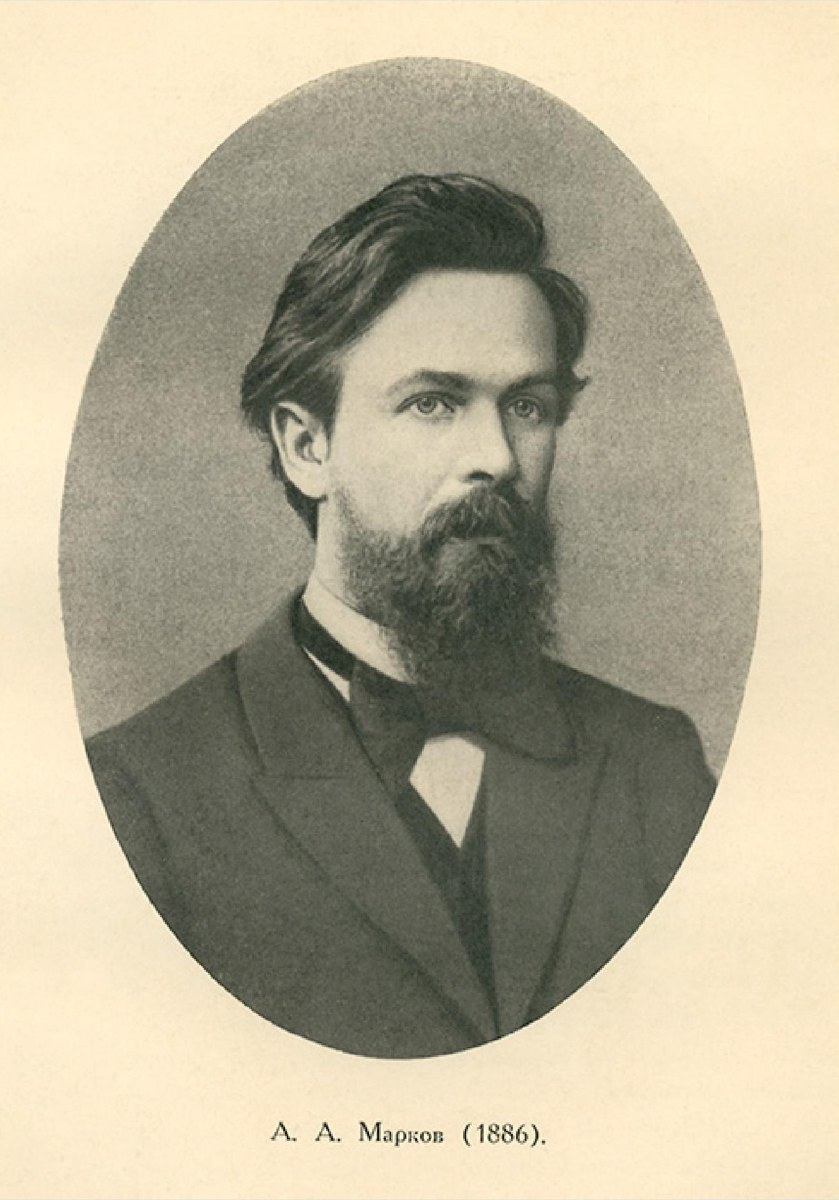
\includegraphics[height=0.42\textheight]{ch7_markov_1886.jpg}\\[1mm]
\imgcap{Andrei Markov (1856--1922), în jurul anului 1886}
\imgcredit{https://commons.wikimedia.org/wiki/File:Andrei_Markov.jpg}{Foto: autor necunoscut (1886); domeniu public; Wikimedia Commons}
\end{column}
\begin{column}{0.64\textwidth}
\begin{itemize}
    \item 1906--1913: lanțurile Markov, o dependență care cere doar starea prezentă
    \item 1970: \refBPSW: verosimilitatea maximă pentru modele Markov ascunse (algoritmul Baum--Welch, un EM înainte de EM); recunoașterea vorbirii \refRab
    \item 1973: \refGQ: regresii cu schimbare de regim în econometrie
    \item 1989--1990: \refHamA{} datează recesiunile din SUA doar din PNB; \refHamB{} dă algoritmul EM; \refKim{} netezitorul
    \item 1993--2006: estimarea bayesiană \refAC, \refChibB, \refFSa; MS-VAR \refKro; MS-GARCH \refGray, \refHMP
\end{itemize}
\end{column}
\end{columns}
\end{frame}


%=============================================================================
\section{Modelul și lanțul Markov}
%=============================================================================

\begin{frame}{Cunoscut din TSA și elemente noi}
\itemsize{\small}
\begin{itemize}
    \item Cunoscut (\atschlink{https://danpele.github.io/Time-Series-Analysis/RO/Cursuri/capitol10_spatiul_starilor_kalman_markov_switching.pdf}{TSA, Capitolul 10}): $y_t = \mu_{S_t} + \varepsilon_t$, matricea de tranziție, duratele așteptate, probabilitățile ergodice, probabilitățile filtrate și netezite din \texttt{statsmodels}
    \begin{itemize}
        \item recesiunile din SUA din PIB, regimurile creșterii din România, efectul anului 2020
    \end{itemize}
    \item Nou: fiecare pas derivat și scris în cod; estimarea ca problemă de optimizare cu capcane; inferența asupra numărului de regimuri
    \begin{itemize}
        \item extensii: tranziții care depind de covariabile, sisteme (MS-VAR), dinamica volatilității (MS-GARCH), estimare bayesiană
    \end{itemize}
    \item \atschlink{https://danpele.github.io/Advanced-Time-Series/RO/Cursuri/capitol2_rupturi_structurale_modele_neliniare.pdf}{Capitolul 2} a împărțit eșantionul după un prag observat (TAR, STAR) sau după o dată (rupturi); aici comutarea este un lanț Markov latent
\end{itemize}
\end{frame}

\begin{frame}{Familia de modele (notația Krolzig)}
\itemsize{\small}
\begin{itemize}
    \item MS($K$)-AR($p$): $y_t = \nu_{S_t} + \sum_{k=1}^p \phi_{k,S_t} y_{t-k} + \sigma_{S_t}\varepsilon_t$, $\varepsilon_t \sim$ i.i.d.\ $N(0, 1)$, $S_t \in \{1, \dots, K\}$
    \begin{itemize}
        \item $S_t$: regimul la momentul $t$, una dintre $K$ valori; $\nu_{S_t}$, $\phi_{k,S_t}$, $\sigma_{S_t}$: termenul liber, coeficienții AR($p$) și abaterea standard a șocului în regimul curent
        \item $S_t$ un lanț Markov omogen, $p_{ij} = \Pr(S_t = j \mid S_{t-1} = i)$, independent de $\varepsilon$ \refKro; $\mathbf{P} = (p_{ij})$: matricea de tranziție, cu suma pe fiecare rînd egală cu 1
    \end{itemize}
    \item Parametrii care comută dau numele:
    \begin{itemize}
        \item \textbf{MSI}: termenul liber $\nu$; \textbf{MSIH}: termenul liber și varianța; \textbf{MSIAH}: termenul liber, coeficienții AR și varianța
        \item \textbf{MSM} (Hamilton 1989): comută \emph{media} $\mu_{S_t}$, $y_t - \mu_{S_t} = \sum_k \phi_k(y_{t-k} - \mu_{S_{t-k}}) + \sigma\varepsilon_t$
    \end{itemize}
    \item MSI: după o comutare media se ajustează treptat; MSM: sare imediat; MSM cere regimurile a $p + 1$ perioade
    \item Cazuri particulare: $p_{ij} = \pi_j$ pentru orice $i$ dă un amestec i.i.d.; o matrice $\mathbf{P}$ superior triunghiulară dă un model cu puncte de schimbare \refChibC
\end{itemize}
\end{frame}

\begin{frame}{Lanțul: ergodicitate, durate, persistență}
\itemsize{\small}
\begin{itemize}
    \item Probabilitățile ergodice: $\boldsymbol\pi'\mathbf{P} = \boldsymbol\pi'$, $\mathbf{1}'\boldsymbol\pi = 1$; pentru $K = 2$, $\pi_1 = (1 - p_{22})/(2 - p_{11} - p_{22})$
    \begin{itemize}
        \item $\boldsymbol\pi$: proporția pe termen lung a timpului petrecut în fiecare regim; $\mathbf{1}$: un vector de unități
        \item duratele sînt geometrice: $\Pr(D_i = d) = p_{ii}^{d-1}(1 - p_{ii})$, $\E D_i = 1/(1 - p_{ii})$ (fără memorie); $D_i$: numărul de perioade cît durează o vizită în regimul $i$
    \end{itemize}
    \item Reprezentarea AR(1) \refHam, \S22.2: $\xi_t = \mathbf{1}\{S_t = 1\}$ verifică $\xi_t = (1 - p_{22}) + \lambda\xi_{t-1} + v_t$, $\lambda = p_{11} + p_{22} - 1$
    \begin{itemize}
        \item $\mathbf{1}\{\cdot\}$: indicatorul (1 dacă este adevărat, 0 altfel); $v_t$: inovația; este o diferență de martingală, dar nu este independentă de trecut (varianța ei depinde de $S_{t-1}$)
        \item $\Pr(S_{t+h} = 1 \mid S_t) \to \pi_1$ cu viteza $\lambda^h$: $\lambda$ este persistența procesului de regim
    \end{itemize}
    \item Dependența de durată (recesiuni care se încheie mai probabil cu cît durează mai mult) cere o stare extinsă sau un lanț semi-Markov \refMM
\end{itemize}
\end{frame}

\begin{frame}{Duratele și viteza de amestecare}
\itemsize{\footnotesize}
\begin{center}
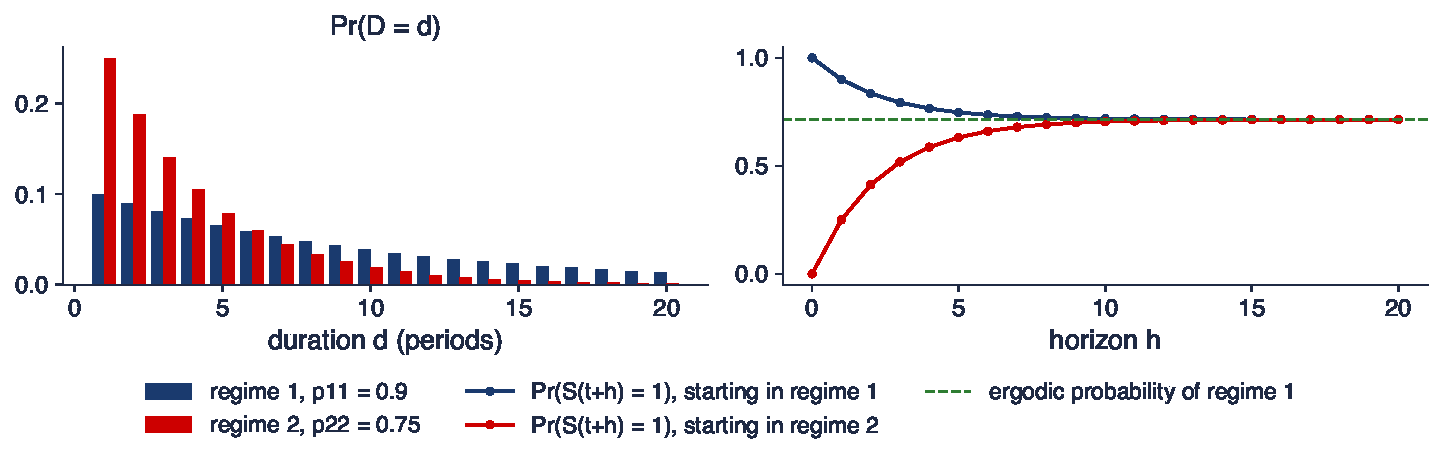
\includegraphics[width=0.97\textwidth,height=0.59\textheight,keepaspectratio]{ats_ch7_chain.pdf}
\end{center}
\vspace{-0.25cm}
\begin{itemize}
    \item $p_{11} = 0{,}9$, $p_{22} = 0{,}75$: durate așteptate de 10 și 4 perioade; $\pi_1 = 0{,}714$; $\lambda = 0{,}65$
    \item Distanța față de probabilitatea ergodică scade cu factorul $\lambda$ în fiecare perioadă: după 10 perioade regimul de pornire este aproape uitat
\end{itemize}
\quantlet{ATS\_ch7\_hamilton}{\qlurl{ATS_ch7_hamilton}}
\end{frame}

\begin{frame}{Recapitulare: modelul}
\itemsize{\small}
\begin{itemize}
    \item Un lanț Markov latent alege parametrii ecuației observațiilor
    \item Literele lui Krolzig spun ce comută; MSM cere starea extinsă
    \item Duratele sînt geometrice; $\lambda = p_{11} + p_{22} - 1$ măsoară persistența
\end{itemize}
\end{frame}


%=============================================================================
\section{Filtrul Hamilton și netezitorul Kim}
%=============================================================================

\begin{frame}{Filtrul Hamilton, derivat}
\itemsize{\small}
\begin{itemize}
    \item Notație: $Y_t = (y_1, \dots, y_t)$, $\hat\xi_{t|s}$ vectorul $\Pr(S_t = j \mid Y_s)$ de dimensiune $K$, $\eta_t$ vectorul densităților $f(y_t \mid S_t = j, Y_{t-1})$
    \begin{itemize}
        \item \textbf{predicția} (probabilitatea totală, proprietatea Markov): $\hat\xi_{t|t-1} = \mathbf{P}'\hat\xi_{t-1|t-1}$
        \item \textbf{actualizarea} (Bayes): $\hat\xi_{t|t} = \dfrac{\hat\xi_{t|t-1}\odot\eta_t}{\mathbf{1}'(\hat\xi_{t|t-1}\odot\eta_t)}$
        \item \textbf{verosimilitatea}: $f(y_t \mid Y_{t-1}) = \mathbf{1}'(\hat\xi_{t|t-1}\odot\eta_t)$, deci $\ln L = \sum_t \ln f(y_t \mid Y_{t-1})$
    \end{itemize}
    \item Pornire: $\hat\xi_{1|0} = \boldsymbol\pi$ (ergodic) sau un parametru liber; $\odot$ este produsul element cu element
    \item Aceeași structură ca filtrul Kalman (\atschlink{https://danpele.github.io/Advanced-Time-Series/RO/Cursuri/capitol6_modele_spatiul_starilor_filtrare_bayesiana.pdf}{Capitolul 6}): predicție, actualizare, descompunerea erorilor de predicție; aici starea este discretă, iar actualizarea este exactă
\end{itemize}
\end{frame}

\begin{frame}{Aspecte numerice și cost}
\itemsize{\small}
\begin{itemize}
    \item Densitățile ajung sub limita reprezentabilă (de exemplu $10^{-300}$ după o valoare extremă): lucrăm cu $\ln\eta_t$ și scădem $m_t = \max_j \ln\eta_{jt}$
    \begin{itemize}
        \item $\ln f(y_t \mid Y_{t-1}) = m_t + \ln\sum_j \hat\xi_{j,t|t-1}e^{\ln\eta_{jt} - m_t}$ (log-sum-exp); vectorul filtrat nu se schimbă
    \end{itemize}
    \item Cost: $O(TK^2)$; la MSM-AR($p$) starea este $(S_t, \dots, S_{t-p})$, $M = K^{p+1}$ ($32$ pentru $K = 2$, $p = 4$ ale lui Hamilton)
    \begin{itemize}
        \item matricea de tranziție extinsă este rară: din $(i_0, \dots, i_p)$ se trece doar în $(j, i_0, \dots, i_{p-1})$, cu probabilitatea $p_{i_0 j}$
        \item MSI-AR($p$) cere doar $K$ stări: valorile cu lag ale lui $y$ intră ca regresori
    \end{itemize}
    \item Filtrul nostru numpy și \texttt{statsmodels} dau aceeași log-verosimilitate, la precizia mașinii, cînd distribuția inițială este aceeași
\end{itemize}
\end{frame}

\begin{frame}{Netezitorul Kim, derivat}
\itemsize{\small}
\begin{itemize}
    \item Scopul: $\hat\xi_{t|T}$, probabilitățile regimurilor date fiind toate datele \refKim
    \begin{itemize}
        \item pasul-cheie: $\Pr(S_t = i \mid S_{t+1} = j, Y_T) = \Pr(S_t = i \mid S_{t+1} = j, Y_t)$: dat fiind $S_{t+1}$, valorile viitoare ale lui $y$ nu aduc informație suplimentară despre $S_t$
        \item exact pentru MSI/MSIH/MSM pe starea extinsă; aproximare doar cînd starea are și o parte continuă (Kim 1994, \atschlink{https://danpele.github.io/Advanced-Time-Series/RO/Cursuri/capitol6_modele_spatiul_starilor_filtrare_bayesiana.pdf}{Capitolul 6})
        \item demonstrația pasului-cheie: \atsapplink{atsapp2}{atssrc1}{Anexa}  % applink: netezitorul Kim, pasul Markov
    \end{itemize}
    \item Bayes pentru pereche: $\Pr(S_t = i, S_{t+1} = j \mid Y_T) = \dfrac{\hat\xi_{i,t|t}\,p_{ij}}{\hat\xi_{j,t+1|t}}\,\hat\xi_{j,t+1|T}$
    \begin{itemize}
        \item sumăm după $j$: $\hat\xi_{t|T} = \hat\xi_{t|t}\odot\left[\mathbf{P}(\hat\xi_{t+1|T}\oslash\hat\xi_{t+1|t})\right]$, înapoi de la $\hat\xi_{T|T}$; $\oslash$: împărțirea element cu element
    \end{itemize}
    \item Probabilitățile comune ale perechii $(S_t, S_{t+1})$ sînt pasul E al algoritmului EM; eșantionarea în locul sumării dă FFBS (secțiunea 7)
\end{itemize}
\end{frame}

\begin{frame}{Trei probabilități, trei întrebări}
\itemsize{\small}
\begin{itemize}
    \item Probabilitatea \textbf{prezisă} $\hat\xi_{t+1|t}$: ce așteaptă un prognozator pentru perioada următoare; intră în densitatea de prognoză
    \item Probabilitatea \textbf{filtrată} $\hat\xi_{t|t}$: ce se putea ști la $t$; semnalul în timp real (Chauvet și Piger 2008)
    \begin{itemize}
        \item datarea în timp real se evaluează cu probabilități filtrate și cu edițiile datelor, niciodată cu cele netezite
    \end{itemize}
    \item Probabilitatea \textbf{netezită} $\hat\xi_{t|T}$: răspunsul istoricului; folosește viitorul și se revizuiește pe măsură ce sosesc date
    \begin{itemize}
        \item datarea regimurilor trecute și ponderile pasului M
    \end{itemize}
    \item Confuzia lor este cea mai frecventă eroare în lucrările aplicate: o probabilitate netezită nu este o prognoză
\end{itemize}
\end{frame}

\begin{frame}{Recapitulare: filtru și netezitor}
\itemsize{\small}
\begin{itemize}
    \item Filtrul: predicție cu $\mathbf{P}'$, actualizare cu Bayes, acumularea log-verosimilității
    \item Netezitorul: o trecere înapoi cu raportul dintre probabilitățile netezite și cele prezise
    \item Se lucrează în logaritmi; starea se extinde doar cînd comută media
\end{itemize}
\end{frame}


%=============================================================================
\section{Estimarea: EM și verosimilitatea maximă numerică}
%=============================================================================

\begin{frame}{EM: verosimilitatea datelor complete}
\itemsize{\small}
\begin{itemize}
    \item Dacă $S_1, \dots, S_T$ ar fi observate, log-verosimilitatea s-ar separa \refDLR, \refHamB:
    \begin{itemize}
        \item $\ln L_c = \sum_j \mathbf{1}\{S_1 = j\}\ln\rho_j + \sum_{t\ge2}\sum_{i,j}\mathbf{1}\{S_{t-1} = i, S_t = j\}\ln p_{ij} + \sum_t\sum_j \mathbf{1}\{S_t = j\}\ln\eta_{jt}(\theta_j)$
        \item $\rho_j = \Pr(S_1 = j)$: probabilitățile inițiale; $\eta_{jt}(\theta_j)$: densitatea lui $y_t$ în regimul $j$, cu parametrii $\theta_j$
        \item numărarea tranzițiilor și regresii regim cu regim: forme închise
    \end{itemize}
    \item \textbf{Pasul E}: înlocuim indicatorii cu speranțele lor condiționate de $Y_T$ și de $\theta^{(m)}$ curent ($m$: iterația)
    \begin{itemize}
        \item $\hat\xi_{j,t|T}$ și $\hat\xi_{ij,t|T} = \Pr(S_{t-1} = i, S_t = j \mid Y_T)$: exact ieșirea netezitorului Kim
    \end{itemize}
    \item Baum et al.\ (1970) au derivat aceeași recursie pentru modelele Markov ascunse (algoritmul forward--backward)
\end{itemize}
\end{frame}

\begin{frame}{EM: pasul M în formă închisă}
\itemsize{\small}
\begin{itemize}
    \item Tranzițiile: $p_{ij}^{(m+1)} = \dfrac{\sum_{t=2}^T \hat\xi_{ij,t|T}}{\sum_{t=2}^T \hat\xi_{i,t-1|T}}$ (tranziții așteptate raportate la vizite așteptate); $\rho^{(m+1)} = \hat\xi_{1|T}$
    \item Coeficienți care comută (MSIAH): cele mai mici pătrate ponderate $\beta_j^{(m+1)} = (X'W_jX)^{-1}X'W_jy$, $W_j = \mathrm{diag}(\hat\xi_{j,t|T})$; $X$: liniile $x_t'$ (constanta și lagurile), $y$: observațiile; fiecare dată contează cu probabilitatea de a fi în regimul $j$
    \item Varianțele: $\sigma_j^{2(m+1)} = \sum_t\hat\xi_{j,t|T}(y_t - x_t'\beta_j)^2/\sum_t\hat\xi_{j,t|T}$; MS-VAR: același lucru cu matrice
    \item Coeficienți comuni (MSIH-AR): o singură regresie ponderată stivuită, cu ponderile $\hat\xi_{j,t|T}/\sigma_j^2$ (un pas M condiționat, ECM)
    \item MSM-AR: $\mu$ și $\phi$ apar ca produse, deci nu există formă închisă: maximizare numerică (sau EM cu un pas M numeric)
    \item Derivarea pasului M pentru $\mathbf{P}$ și a monotoniei EM: \atsapplink{atsapp1}{atssrc2}{Anexa}  % applink: EM pentru lanțul Markov
\end{itemize}
\end{frame}

\begin{frame}{EM și verosimilitatea maximă numerică în practică}
\itemsize{\small}
\begin{itemize}
    \item EM nu scade niciodată verosimilitatea, este robust departe de optim, dar lent în apropierea lui (convergență liniară)
    \begin{itemize}
        \item monotonia cere ca $\rho$ să fie un parametru liber; cu $\rho = \boldsymbol\pi(\mathbf{P})$ pasul M pentru $\mathbf{P}$ este doar aproximativ
    \end{itemize}
    \item Verosimilitatea maximă numerică: BFGS pe parametri fără restricții ($\ln\sigma_j^2$, logit-urile lui $p_{ij}$); erorile standard din hessiană prin metoda delta
    \begin{itemize}
        \item în practică: EM din multe puncte de pornire, apoi o rafinare de tip Newton și hessiana
    \end{itemize}
    \item Verosimilitatea este nemărginită: $\sigma_j \to 0$ în jurul unei observații, cu $p_{jj} \to 0$, dă $\ln L \to \infty$
    \begin{itemize}
        \item remedii: o limită inferioară pentru $\sigma_j/\sigma_k$ \refHath, distribuții a priori (secțiunea 7) sau respingerea regimurilor care durează o singură perioadă
    \end{itemize}
    \item Erorile standard lîngă frontieră ($p_{ii} \approx 1$) nu sînt de încredere: raportați verosimilitatea de profil sau intervale bootstrap
\end{itemize}
\end{frame}

\begin{frame}{EM din 30 de puncte de pornire}
\itemsize{\footnotesize}
\begin{center}
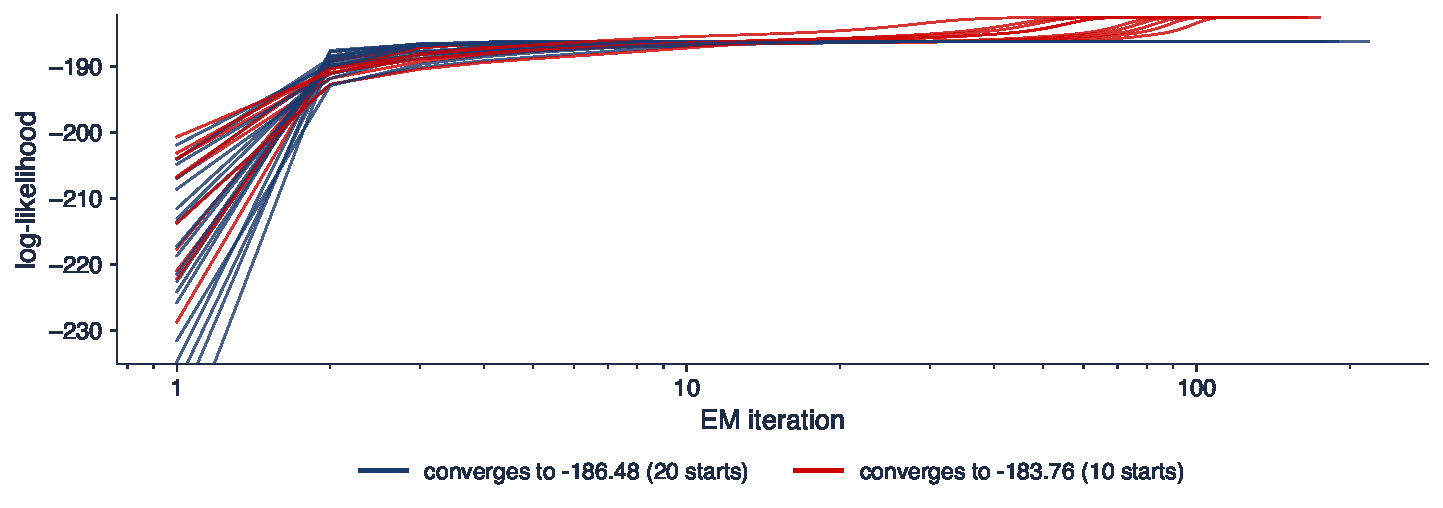
\includegraphics[width=0.97\textwidth,height=0.65\textheight,keepaspectratio]{ats_ch7_em.pdf}
\end{center}
\vspace{-0.25cm}
\begin{itemize}
    \item MSIH(2)-AR(1) pe datele PNB ale lui Hamilton: termen liber și varianță care comută, coeficient AR(1) comun; puncte de pornire aleatoare; scară logaritmică pentru iterații
\end{itemize}
\quantlet{ATS\_ch7\_estimation}{\qlurl{ATS_ch7_estimation}}
\end{frame}

\begin{frame}{Interpretarea traiectoriilor EM}
\itemsize{\small}
\begin{itemize}
    \item 2 limite (log-verosimilitatea, numărul de puncte de pornire): \ensuremath{-}186{,}48 (20); \ensuremath{-}183{,}76 (10); în mediană 159 de iterații, cel mult 216
    \item Cea mai înaltă (\ensuremath{-}183{,}76) este \textbf{degenerată}: un regim cu $\sigma^2 = 0{,}049$, $p_{11}$ $<10^{-9}$ și media 1{,}11, folosit de 29 de trimestre izolate
    \item \texttt{statsmodels} (20 de căutări aleatoare) raportează \ensuremath{-}185{,}73, un al treilea maxim local, pe care niciunul dintre punctele noastre de pornire nu l-a atins
    \item Lecția: raportați schema punctelor de pornire, toate maximele locale și motivul pentru care cel ales are sens economic
\end{itemize}
\end{frame}

\begin{frame}{Identificare și schimbarea etichetelor}
\itemsize{\small}
\begin{itemize}
    \item Verosimilitatea este invariantă la cele $K!$ permutări ale etichetelor: $(\theta_1, \theta_2, \mathbf{P})$ și $(\theta_2, \theta_1, \mathbf{\Pi P\Pi}')$ se potrivesc la fel de bine
    \begin{itemize}
        \item pentru verosimilitatea maximă este inofensiv: alegem un mod și numim regimurile după o ordonare ($\mu_1 < \mu_2$ sau $\sigma_1 < \sigma_2$)
        \item pentru MCMC nu este: eșantionatorul sare între moduri, iar media a posteriori a lui $\mu_1$ amestecă regimurile \refCHR, \refSte
    \end{itemize}
    \item Identificarea eșuează și local: $K$ regimuri cu $\theta_i = \theta_j$ sau un regim nevizitat lasă $\mathbf{P}$ neidentificat
    \begin{itemize}
        \item aceasta este rădăcina problemei de testare din secțiunea următoare
    \end{itemize}
    \item Regimurile statistice nu sînt neapărat regimuri economice: aceleași date de PIB dau recesiuni (MSM), ere de volatilitate (MSIH) sau valori extreme izolate
\end{itemize}
\end{frame}

\begin{frame}{Recapitulare: estimarea}
\itemsize{\small}
\begin{itemize}
    \item EM = netezitorul Kim + regresii ponderate + numărarea tranzițiilor
    \item Multe puncte de pornire, apoi o rafinare numerică; inspectați fiecare maxim local
    \item Maximele degenerate și schimbarea etichetelor sînt trăsături ale amestecurilor, nu erori ale codului
\end{itemize}
\end{frame}


%=============================================================================
\section{Numărul de regimuri: testare și selecție}
%=============================================================================

\begin{frame}{Testul LR nestandard}
\itemsize{\small}
\begin{itemize}
    \item $H_0$: un singur regim ($\mu_1 = \mu_2$, $\sigma_1 = \sigma_2$) față de $H_1$: două regimuri
    \begin{itemize}
        \item (i) sub $H_0$, $p_{11}$ și $p_{22}$ \textbf{nu sînt identificați}: parametri de perturbare prezenți doar sub $H_1$, problema Davies din \atschlink{https://danpele.github.io/Advanced-Time-Series/RO/Cursuri/capitol2_rupturi_structurale_modele_neliniare.pdf}{Capitolul 2} \refDav
        \item (ii) ipoteza nulă se poate scrie $p_{11} = 1$: un parametru pe \textbf{frontieră}
        \item (iii) scorul în raport cu $\mu_2 - \mu_1$ este \textbf{identic zero} sub $H_0$: matricea informațională este singulară
    \end{itemize}
    \item Fiecare dintre cele trei încalcă una dintre condițiile pentru $2\ln\Lambda \to \chi^2_q$ ($\Lambda$: raportul de verosimilitate; $q$: numărul de restricții): numărarea parametrilor nu dă valoarea critică
    \item Aceeași structură ca testarea liniarității față de TAR sau STAR (\atschlink{https://danpele.github.io/Advanced-Time-Series/RO/Cursuri/capitol2_rupturi_structurale_modele_neliniare.pdf}{Capitolul 2}), cu o comutare latentă în locul uneia observate
\end{itemize}
\end{frame}

\begin{frame}{Soluțiile din literatură}
\itemsize{\small}
\begin{itemize}
    \item \refHan: tratează verosimilitatea ca un proces empiric în parametrii de perturbare și mărginește LR standardizat; conservator, greu de calculat
    \begin{itemize}
        \item aplicat modelului PNB al lui Hamilton: nicio dovadă împotriva unui singur regim la nivelurile uzuale
    \end{itemize}
    \item \refGar: distribuția asimptotică sub $H_0$ a statisticii sup-LR pentru modele cu medie (și varianță) care comută, cu valori critice tabelate
    \item \refCW: quasi-LR față de un amestec cu două componente (o comutare i.i.d.\ are același comportament sub $H_0$)
    \item \refCHP: un test optim de tip scor față de schimbarea de regim de tip Markov, care cere doar modelul nul
    \item În practică: \textbf{bootstrap parametric} al LR
    \begin{itemize}
        \item simulăm din modelul nul estimat; reestimăm ambele modele (cu mai multe puncte de pornire) pe fiecare eșantion
        \item $p = (1 + \#\{LR^* \ge LR\})/(B + 1)$; $LR^*$: cele $B$ statistici bootstrap; $\#$: numărul celor mai mari decît $LR$
    \end{itemize}
    \item Selecție în loc de testare: AIC, BIC, HQ sau factori Bayes prin verosimilitatea marginală \refChibA
\end{itemize}
\end{frame}

\begin{frame}{Distribuția bootstrap a statisticii LR sub ipoteza nulă}
\itemsize{\footnotesize}
\begin{center}
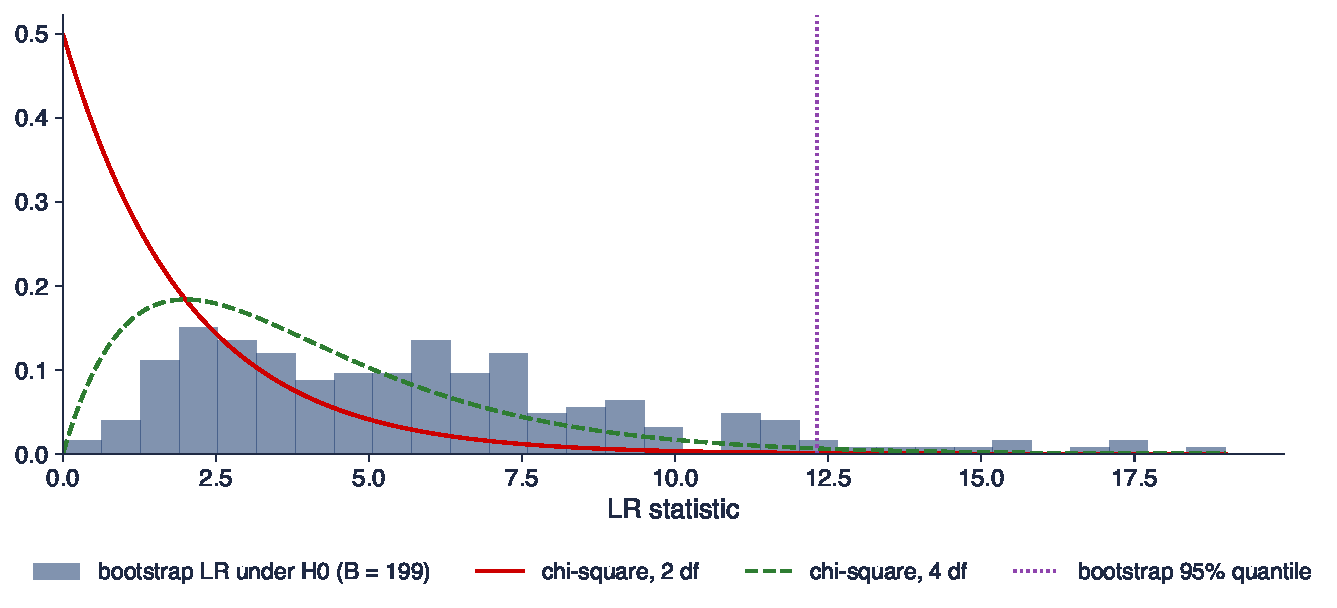
\includegraphics[width=0.97\textwidth,height=0.65\textheight,keepaspectratio]{ats_ch7_lrtest.pdf}
\end{center}
\vspace{-0.25cm}
\begin{itemize}
    \item Creșterea PIB-ului SUA, T2 1947--T4 2019 ($T = 290$): $H_0$ AR(1) Gaussian, $H_1$ MSIH(2)-AR(1); 199 de eșantioane simulate din AR(1) estimat, ambele modele reestimate, EM cu 4 puncte de pornire
\end{itemize}
\quantlet{ATS\_ch7\_estimation}{\qlurl{ATS_ch7_estimation}}
\end{frame}

\begin{frame}{Interpretarea testului}
\itemsize{\small}
\begin{itemize}
    \item Cuantila bootstrap de 95\% este 12{,}32, față de 5{,}99 ($\chi^2_2$) și 9{,}49 ($\chi^2_4$); media extragerilor sub $H_0$ 5{,}79: numărarea parametrilor dă o valoare critică greșită
    \item LR observat = 71{,}7, p-value-ul bootstrap 0{,}005 (cea mai mică posibilă cu $B = 199$): două regimuri
    \item Dar ce regimuri? Abaterile standard 0{,}46 și 1{,}11 pp, $p_{ii}$ = 0{,}990 și 0{,}985: ere de volatilitate (Marea Moderație), nu recesiuni
    \item BIC: 755{,}5 ($K = 1$), 706{,}4 ($K = 2$), 734{,}7 ($K = 3$); AIC: 744{,}5; 680{,}8; 687{,}0
\end{itemize}
\end{frame}

\begin{frame}{Recapitulare: numărul de regimuri}
\itemsize{\small}
\begin{itemize}
    \item Parametri de perturbare neidentificați, o frontieră și un scor nul: nicio limită chi-pătrat
    \item Folosiți p-value-uri bootstrap sau valori critice de tip Garcia; criterii informaționale pentru selecție
    \item Un test semnificativ spune că modelul se potrivește mai bine, nu că regimurile înseamnă ce am sperat
\end{itemize}
\end{frame}


%=============================================================================
\section{Studiu de caz: Hamilton (1989) și ciclul economic}
%=============================================================================

\begin{frame}{Lucrarea}
\itemsize{\footnotesize}
\begin{columns}[T]
\begin{column}{0.36\textwidth}
\centering
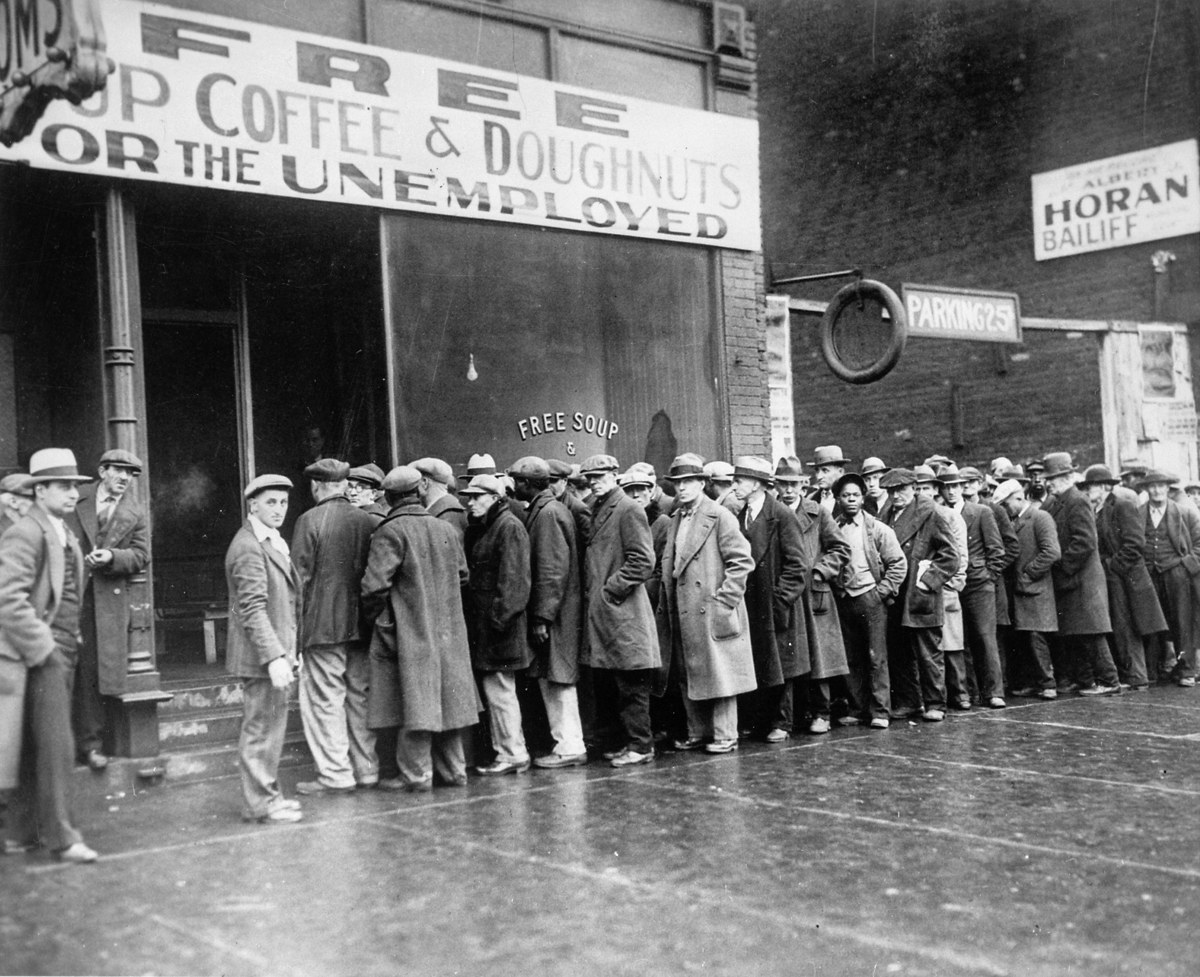
\includegraphics[height=0.34\textheight]{ch7_soup_kitchen_1931.jpg}\\[1mm]
\imgcap{Chicago, februarie 1931: regimul de care se teme orice prognozator}
\imgcredit{https://commons.wikimedia.org/wiki/File:Unemployed_men_queued_outside_a_depression_soup_kitchen_opened_in_Chicago_by_Al_Capone,_02-1931_-_NARA_-_541927.jpg}{Foto: US National Archives (1931); domeniu public; Wikimedia Commons}
\end{column}
\begin{column}{0.62\textwidth}
\begin{itemize}
    \item \refHamA, secțiunea 4: PNB real al SUA, 100 $\times$ variația logaritmului, T2 1951--T4 1984, MSM(2)-AR(4)
    \item Ecuația (4.3): $y_t - \mu_{S_t} = \sum_{k=1}^4\phi_k(y_{t-k} - \mu_{S_{t-k}}) + \sigma\varepsilon_t$; estimațiile în Tabelul I
    \item Afirmația: datele în care regimul de creștere scăzută este probabil coincid cu recesiunile NBER, deși datele NBER nu au fost folosite
    \item Replicăm pe setul lui de date, comparăm numpy cu \texttt{statsmodels}, apoi reestimăm pe PIB-ul de azi
\end{itemize}
\end{column}
\end{columns}
\end{frame}

\begin{frame}{Replicare: datele lui Hamilton, două implementări}
\itemsize{\small}
\begin{center}
\scriptsize
\begin{tabular}{lcccccccc}
\toprule
\textbf{Estimarea} & $\mu_0$ & $\mu_1$ & $\phi_1$ & $\phi_2$ & $\phi_3$ & $\phi_4$ & $\sigma$ & $\ln L$ \\
\midrule
numpy & \ensuremath{-}0{,}359 & 1{,}164 & 0{,}013 & \ensuremath{-}0{,}058 & \ensuremath{-}0{,}247 & \ensuremath{-}0{,}213 & 0{,}769 & \ensuremath{-}181{,}26 \\
(eroarea standard) & (0{,}265) & (0{,}075) & (0{,}120) & (0{,}138) & (0{,}107) & (0{,}111) & &  \\
statsmodels & 1{,}164 & \ensuremath{-}0{,}359 & 0{,}013 & \ensuremath{-}0{,}058 & \ensuremath{-}0{,}247 & \ensuremath{-}0{,}213 & 0{,}769 & \ensuremath{-}181{,}26 \\
\bottomrule
\end{tabular}
\end{center}
\begin{itemize}
    \item Tranziții: $p_{00} = 0{,}755$ (rămînerea în regimul scăzut), $p_{11} = 0{,}904$; durate așteptate de 4{,}1 și 10{,}4 trimestre; $T = 131$ după 4 laguri
    \item Cea mai mare diferență între cele două traiectorii ale probabilităților netezite: $<10^{-4}$
    \item Estimarea: BFGS pe starea extinsă de 32 de combinații de regimuri, 8 puncte de pornire aleatoare; erorile standard din hessiana numerică
\end{itemize}
\end{frame}

\begin{frame}{Regimurile lui Hamilton atunci și acum}
\itemsize{\footnotesize}
\begin{center}
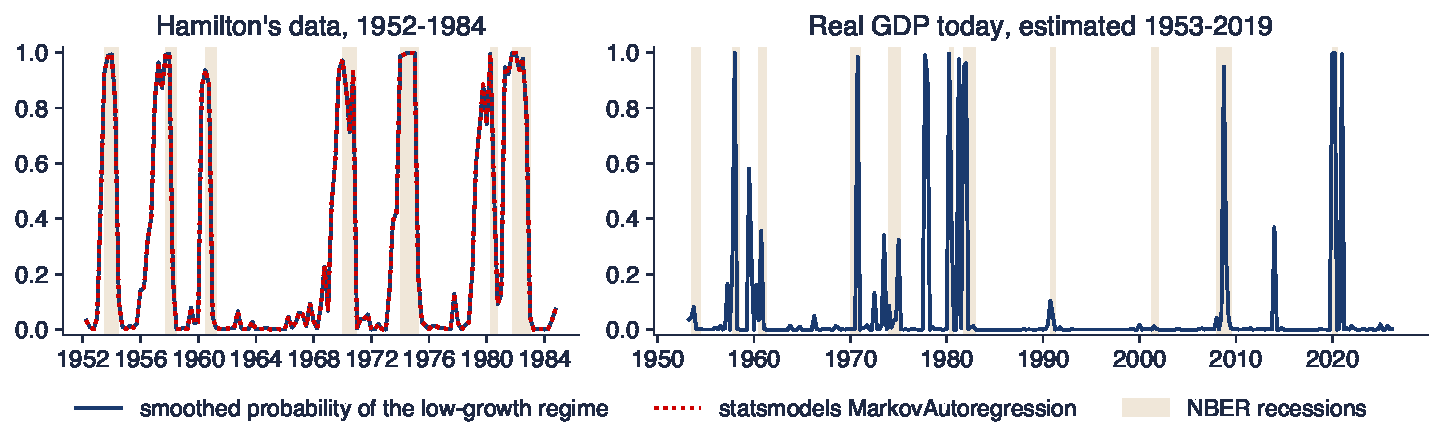
\includegraphics[width=0.97\textwidth,height=0.57\textheight,keepaspectratio]{ats_ch7_hamilton89.pdf}
\end{center}
\vspace{-0.25cm}
\begin{itemize}
    \item Stînga: probabilitatea netezită a regimului de creștere scăzută pe datele lui Hamilton. Dreapta: aceeași specificație pe GDPC1 de azi, estimată pe T2 1953--T4 2019 ($T = 267$), probabilități pînă în T2 2026 cu aceiași parametri
\end{itemize}
\quantlet{ATS\_ch7\_hamilton}{\qlurl{ATS_ch7_hamilton}}
\end{frame}

\begin{frame}{Interpretarea replicării}
\itemsize{\small}
\begin{itemize}
    \item Pe datele lui, regimul urmărește datările NBER: QPS 0{,}179 și concordanță de 89\% (probabilitate peste 0,5 comparată cu trimestrele NBER) \refDR, \refHP
    \item Pe datele de azi, regimul scăzut își schimbă natura: media \ensuremath{-}1{,}22\%, $p_{00} = 0{,}26$ (durata 1{,}4 trimestre): căderi bruște izolate, nu recesiuni
    \item Prinde T4 2008 (0{,}95) și T2 2020 (1{,}00), dar nu 2001 (cel mult 0{,}01); QPS 0{,}229 pe 37 de trimestre NBER
    \item După 1984 recesiunile sînt mai rare și mai blînde (Marea Moderație): un model fix cu două medii își pierde puterea; de aici TVTP, MSIH și trei regimuri
\end{itemize}
\end{frame}

\begin{frame}{Datarea în pseudo timp real}
\itemsize{\footnotesize}
\begin{center}
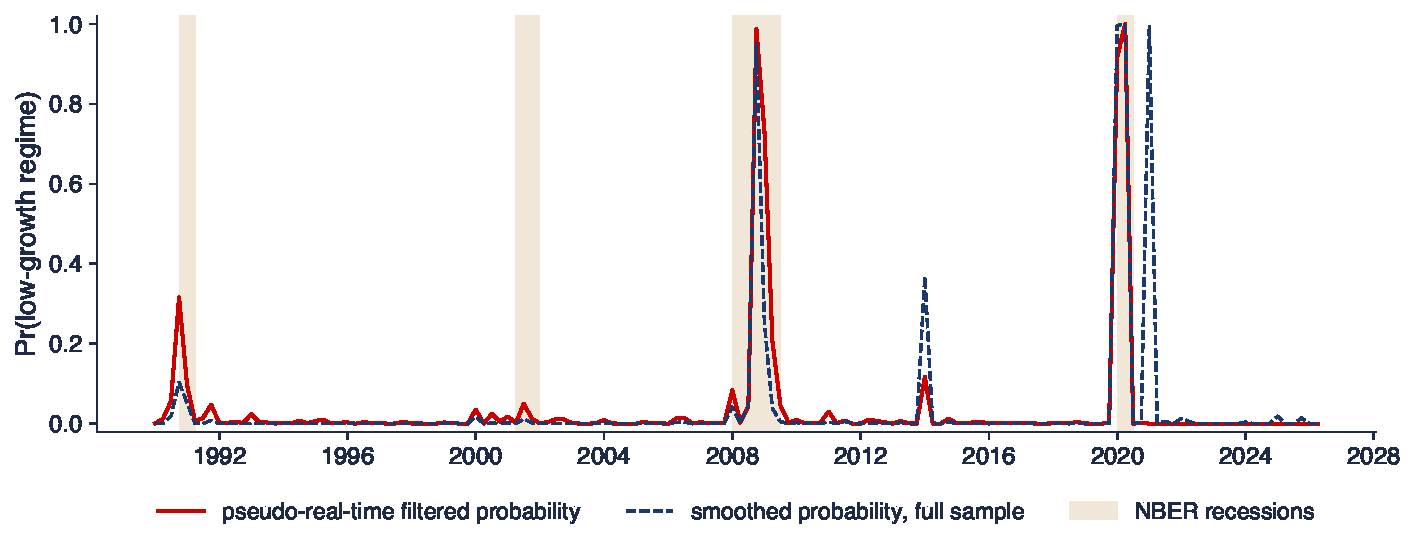
\includegraphics[width=0.97\textwidth,height=0.53\textheight,keepaspectratio]{ats_ch7_realtime.pdf}
\end{center}
\vspace{-0.25cm}
\begin{itemize}
    \item Modelul lui Hamilton reestimat în fiecare an pe datele disponibile atunci (ediția curentă, fără revizuiri ale datelor); probabilitatea filtrată a fiecărui trimestru cu informația de pînă la acel trimestru, 1990--2026
\end{itemize}
\quantlet{ATS\_ch7\_hamilton}{\qlurl{ATS_ch7_hamilton}}
\end{frame}

\begin{frame}{Interpretarea datării în timp real}
\itemsize{\small}
\begin{itemize}
    \item Primul trimestru peste 0,5: 1990--91 niciunul (maximum 0{,}32), 2001 niciunul (maximum 0{,}05), 2008 T4 2008, 2020 T1 2020
    \item QPS înainte de 2020: 0{,}127 în timp real față de 0{,}152 netezit; 0 semnale false peste 0,5
    \item \refCP: cu ediții în timp real, modelele MS semnalează începutul recesiunilor mai repede decît anunțul NBER, dar recesiunile ușoare sînt ratate
    \item Exercițiul nostru avantajează modelul: PIB-ul revizuit de azi nu era disponibil în 2001
\end{itemize}
\end{frame}

\begin{frame}{Recapitulare: studiul de caz Hamilton (1989)}
\itemsize{\small}
\begin{itemize}
    \item Replicat exact pe datele lui cu două implementări independente
    \item Același model pe datele de azi găsește contracții scurte și bruște și ratează 2001
    \item Datarea se judecă în timp real cu probabilități filtrate, nu cu cele netezite
\end{itemize}
\end{frame}


%=============================================================================
\section{Probabilități de tranziție variabile în timp}
%=============================================================================

\begin{frame}{Lanțul dependent de variabile observate}
\itemsize{\small}
\begin{itemize}
    \item \refDLW, \refFil: $p_{ii,t} = \Pr(S_t = i \mid S_{t-1} = i, z_{t-1}) = \dfrac{\exp(z_{t-1}'\gamma_i)}{1 + \exp(z_{t-1}'\gamma_i)}$
    \begin{itemize}
        \item $z_{t-1}$: variabile observate cunoscute la $t - 1$ (cu o constantă); $\gamma_i$: coeficienții lor; funcția logistică menține $p_{ii,t}$ în $(0, 1)$
        \item un indicator avansat, panta curbei randamentelor sau dobînda de politică pot face mai probabil sau mai puțin probabil începutul sau sfîrșitul unei recesiuni
        \item duratele așteptate variază acum în timp; lanțul nu mai este omogen
    \end{itemize}
    \item Filtrul și netezitorul rămîn neschimbate, cu $\mathbf{P}_t$ în locul lui $\mathbf{P}$; EM: pasul M pentru $\gamma_i$ este un logit ponderat (DLW)
    \begin{itemize}
        \item $z_{t-1}$ trebuie să fie predeterminat și să nu depindă de $S_t$; dacă $z$ reacționează la regim, modelul este greșit specificat (comutare endogenă)
    \end{itemize}
    \item Testul tranzițiilor constante: $H_0$: pantele lui $\gamma_i$ sînt zero este un test LR standard, deoarece regimurile există sub ambele ipoteze
\end{itemize}
\end{frame}

\begin{frame}{Replicare: Filardo (1994)}
\itemsize{\small}
\begin{center}
\scriptsize
\begin{tabular}{lcccccc}
\toprule
\textbf{Modelul} & $\mu_0$ & $\mu_1$ & $\gamma_0$ & $\gamma_1$ & $\ln L$ & statsmodels \\
\midrule
TVTP, numpy & \ensuremath{-}0{,}87 & 0{,}50 & (1{,}49; \ensuremath{-}1{,}09) & (4{,}33; 1{,}75) & \ensuremath{-}586{,}20 & \ensuremath{-}586{,}20 \\
(eroarea standard) & & & (0{,}48; 0{,}62) & (0{,}76; 0{,}52) & &  \\
tranziții constante & & 2{,}77 & $p_{00} = 0{,}983$ & $p_{11} = 0{,}14$ & \ensuremath{-}590{,}67 &  \\
\bottomrule
\end{tabular}
\end{center}
\begin{itemize}
    \item Creșterea producției industriale din SUA, lunar, $T = 513$ (datele lui Filardo); MSM(2)-AR(4); $z_{t-1}$ = (1, creșterea indicatorului compozit avansat)
    \item LR pentru TVTP față de tranziții constante: 8{,}94 ($p = 0{,}011$, 2 restricții)
    \item Maximul cu tranziții constante nu este un ciclu economic: un regim cu medie mare (2{,}77\% pe lună) care durează aproximativ o lună
\end{itemize}
\end{frame}

\begin{frame}{Probabilități de tranziție determinate de indicatorul avansat}
\itemsize{\footnotesize}
\begin{center}
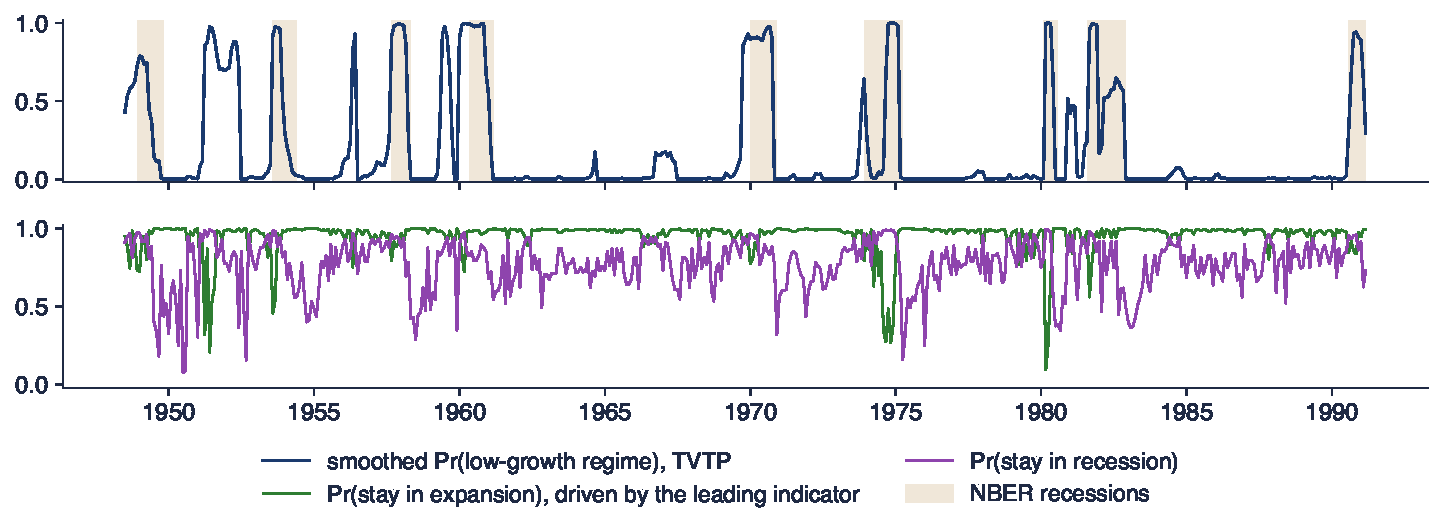
\includegraphics[width=0.97\textwidth,height=0.68\textheight,keepaspectratio]{ats_ch7_tvtp.pdf}
\end{center}
\vspace{-0.25cm}
\begin{itemize}
    \item Sus: probabilitatea netezită a regimului de creștere scăzută; jos: probabilitățile de rămînere în fiecare regim, lună de lună
\end{itemize}
\quantlet{ATS\_ch7\_tvtp}{\qlurl{ATS_ch7_tvtp}}
\end{frame}

\begin{frame}{Interpretarea TVTP}
\itemsize{\small}
\begin{itemize}
    \item Rămînerea în expansiune: mediana 0{,}988, dar coboară pînă la 0{,}10 cînd indicatorul avansat scade puternic: expansiunile se încheie cînd indicatorul se întoarce
    \item Rămînerea în recesiune scade cînd indicatorul crește (panta $\gamma$ \ensuremath{-}1{,}09): revenirile sînt anunțate de indicator
    \item QPS față de lunile NBER 0{,}197, concordanță 88\%
    \item Atenție: indicatorul avansat a fost construit cunoscînd datele NBER; un test în timp real cere edițiile lui
\end{itemize}
\end{frame}


%=============================================================================
\section{Modele VAR cu schimbare de regim}
%=============================================================================

\begin{frame}{MS-VAR și răspunsuri dependente de regim}
\itemsize{\small}
\begin{itemize}
    \item MSIAH($K$)-VAR($p$): $y_t = \nu_{S_t} + \sum_{k=1}^p A_{k,S_t}y_{t-k} + \Sigma_{S_t}^{1/2}\varepsilon_t$, $y_t \in \R^n$ \refKro
    \begin{itemize}
        \item $\nu_{S_t}$, $A_{k,S_t}$, $\Sigma_{S_t}$: vectorul termenilor liberi, matricele lagurilor și covarianța erorilor în regimul curent; $\varepsilon_t \sim N(0, I_n)$
        \item EM: pasul M este o regresie multivariată ponderată pe fiecare regim; $\Sigma_j = \sum_t\hat\xi_{j,t|T}\hat u_{jt}\hat u_{jt}'/\sum_t\hat\xi_{j,t|T}$ ($\hat u_{jt}$: reziduurile regimului $j$)
        \item parametrii cresc ca $K(n + n^2p + n(n + 1)/2)$: shrinkage sau comutare restrînsă (MSIH) în sistemele mai mari (\atschlink{https://danpele.github.io/Advanced-Time-Series/RO/Cursuri/capitol5_bvar_modele_factoriale_nowcasting.pdf}{Capitolul 5})
    \end{itemize}
    \item \textbf{Răspunsuri la impuls dependente de regim} \refEEV: $\partial y_{t+h}/\partial\varepsilon_t$ calculat cu $(A_j, \Sigma_j)$, presupunînd că regimul $j$ persistă pe orizont
    \begin{itemize}
        \item răspunsul complet face media pe traiectoriile viitoare ale regimurilor și depinde de probabilitățile curente ale regimurilor; se obține prin simulare
    \end{itemize}
    \item Comutarea doar în $\Sigma$ identifică șocurile structurale prin heteroscedasticitate (\atschlink{https://danpele.github.io/Advanced-Time-Series/RO/Cursuri/capitol3_modele_var_structurale_proiectii_locale.pdf}{Capitolul 3}); \refSZ{} întreabă dacă politica monetară a SUA a comutat și găsesc mai ales comutări de varianță
\end{itemize}
\end{frame}

\begin{frame}{Un VAR cu două regimuri pentru producție și șomaj}
\itemsize{\footnotesize}
\begin{center}
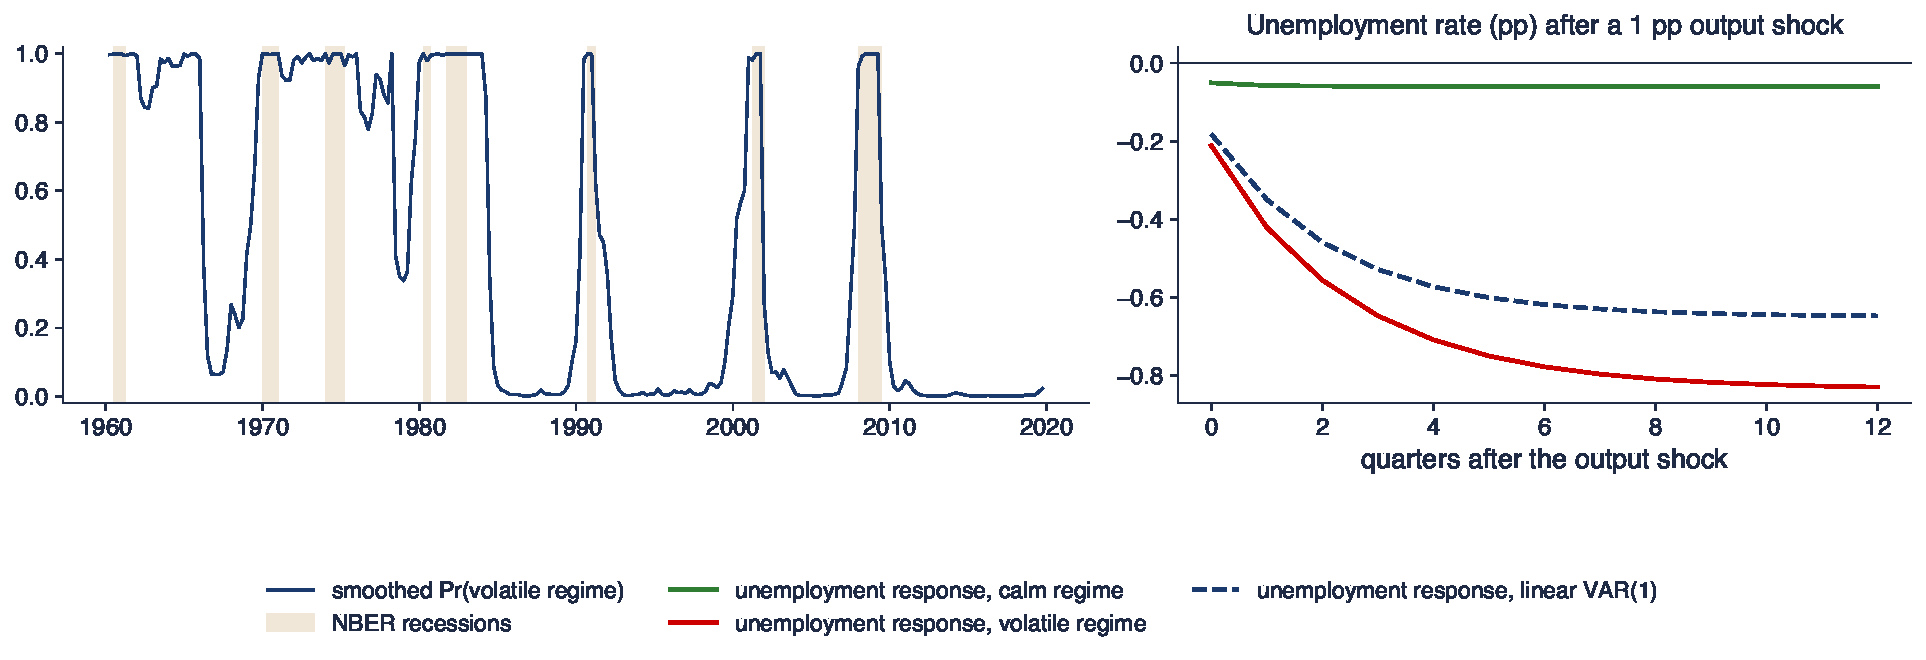
\includegraphics[width=0.97\textwidth,height=0.63\textheight,keepaspectratio]{ats_ch7_msvar.pdf}
\end{center}
\vspace{-0.25cm}
\begin{itemize}
    \item MSIAH(2)-VAR(1) pentru creșterea PIB-ului SUA și variația ratei șomajului, T1 1960--T4 2019 ($T = 239$, 20 de parametri), EM din 12 puncte de pornire; ordinea Cholesky: producția prima; răspunsuri scalate la un șoc de producție de 1 pp
\end{itemize}
\quantlet{ATS\_ch7\_msvar}{\qlurl{ATS_ch7_msvar}}
\end{frame}

\begin{frame}{Interpretarea modelului MS-VAR}
\itemsize{\small}
\begin{itemize}
    \item Regimurile sînt calm și volatil
    \begin{itemize}
        \item abaterea standard a șocului de producție 0{,}42 față de 1{,}02 pp; durate de 21{,}8 și 14{,}3 trimestre
        \item regimul volatil acoperă 83\% din trimestre înainte de 1984, 17\% după și 100\% din trimestrele NBER
    \end{itemize}
    \item Șomajul la 12 trimestre după un șoc de producție de 1 pp: \ensuremath{-}0{,}06 pp (calm), \ensuremath{-}0{,}83 pp (volatil), \ensuremath{-}0{,}65 pp (VAR liniar)
    \item Legea lui Okun depinde de regim
    \begin{itemize}
        \item în regimul calm surprizele de producție aproape nu mișcă șomajul (corelația șocurilor \ensuremath{-}0{,}15, față de \ensuremath{-}0{,}69)
        \item un VAR liniar face media a două transmisii
    \end{itemize}
    \item $\ln L$: \ensuremath{-}166{,}8 (MS-VAR) față de \ensuremath{-}222{,}0 (VAR liniar); răspunsurile dependente de regim presupun că regimul persistă pe orizont
\end{itemize}
\end{frame}


%=============================================================================
\section{Regimuri de volatilitate și MS-GARCH}
%=============================================================================

\begin{frame}{Regimuri în volatilitate}
\itemsize{\footnotesize}
\begin{columns}[T]
\begin{column}{0.3\textwidth}
\centering

\includegraphics[height=0.42\textheight]{ch7_lehman_2007.jpg}\\[1mm]
\imgcap{Lehman Brothers, Times Square, 2007: un regim calm aproape de sfîrșit}
\imgcredit{https://commons.wikimedia.org/wiki/File:Lehman_Brothers_Times_Square_by_David_Shankbone.jpg}{Foto: David Shankbone (2007); CC BY-SA 3.0; Wikimedia Commons}
\end{column}
\begin{column}{0.68\textwidth}
\begin{itemize}
    \item \refLL: schimbările structurale ale varianței deplasează persistența GARCH $\alpha + \beta$ spre 1
    \item \refHS: SWARCH, un ARCH a cărui scală comută după un lanț Markov; mare parte din persistență trece în lanț
    \item MSIH pe randamente: cel mai simplu model cu regimuri de volatilitate, deja un reper util pentru GARCH \refBoll
    \item \atschlink{https://danpele.github.io/Advanced-Time-Series/RO/Cursuri/capitol8_volatilitate_avansata.pdf}{Capitolul 8} dezvoltă măsurile realizate și GARCH multivariat; aici: ce fac regimurile cu GARCH
\end{itemize}
\end{column}
\end{columns}
\end{frame}

\begin{frame}{Problema dependenței de traiectorie}
\itemsize{\small}
\begin{itemize}
    \item MS-GARCH naiv: $h_t = \omega_{S_t} + \alpha_{S_t}\varepsilon_{t-1}^2 + \beta_{S_t}h_{t-1}$
    \begin{itemize}
        \item $h_t$: varianța condiționată; $\varepsilon_{t-1}$: ultimul șoc al randamentului; $\omega$, $\alpha$, $\beta$: parametrii GARCH ai regimului
        \item $h_{t-1}$ depinde la rîndul lui de regim
        \item $h_t$ depinde de întreaga traiectorie $(S_1, \dots, S_t)$: $K^t$ istorii, deci filtrul Hamilton nu se poate aplica ($2^{100} \approx 10^{30}$)
    \end{itemize}
    \item \refGray: comprimă trecutul în $h_{t-1} = \E[\varepsilon_{t-1}^2 \mid Y_{t-2}]$, varianța amestecului: $h_{j,t} = \omega_j + \alpha_j\varepsilon_{t-1}^2 + \beta_j h_{t-1}$
    \begin{itemize}
        \item \refKla: condiționează și pe $S_t$, folosind $\Pr(S_{t-1} \mid S_t, Y_{t-1})$
    \end{itemize}
    \item \refHMP: $K$ procese GARCH rulează în paralel, $h_{j,t} = \omega_j + \alpha_j\varepsilon_{t-1}^2 + \beta_j h_{j,t-1}$; lanțul îl alege pe unul
    \begin{itemize}
        \item fără dependență de traiectorie, verosimilitate exactă, condiții explicite de staționaritate; asimptotica în \refBPR
    \end{itemize}
\end{itemize}
\end{frame}

\begin{frame}{S\&P 500: GARCH comparat cu MS-GARCH}
\itemsize{\small}
\begin{center}
\scriptsize
\begin{tabular}{lccccc}
\toprule
\textbf{Modelul} & $\alpha + \beta$, regimul 1 & $\alpha + \beta$, regimul 2 & $p_{ii}$ & $\ln L$ & BIC \\
\midrule
GARCH(1,1) & 0{,}981 & & & \ensuremath{-}9219{,}9 & 18475{,}0 \\
MS-GARCH (HMP) & 0{,}964 & 0{,}998 & 0{,}959; 0{,}925 & \ensuremath{-}9119{,}1 & 18317{,}5 \\
MS-GARCH (Gray) & 1{,}000 & 0{,}921 & 0{,}981; 0{,}956 & \ensuremath{-}9207{,}4 & 18494{,}1 \\
\bottomrule
\end{tabular}
\end{center}
\begin{itemize}
    \item Randamente logaritmice zilnice (\%), ianuarie 2000 -- septembrie 2026, $T = 6\,714$; inovații Normale, medie comună; verosimilitate maximă numerică în numpy din mai multe puncte de pornire
    \item Regimurile HMP: volatilitatea condiționată medie cît timp regimul este activ 13{,}1\% și 27{,}6\% pe an; durate așteptate de 24 și 13 zile
\end{itemize}
\end{frame}

\begin{frame}{Volatilitatea condiționată și regimul de volatilitate ridicată}
\itemsize{\footnotesize}
\begin{center}
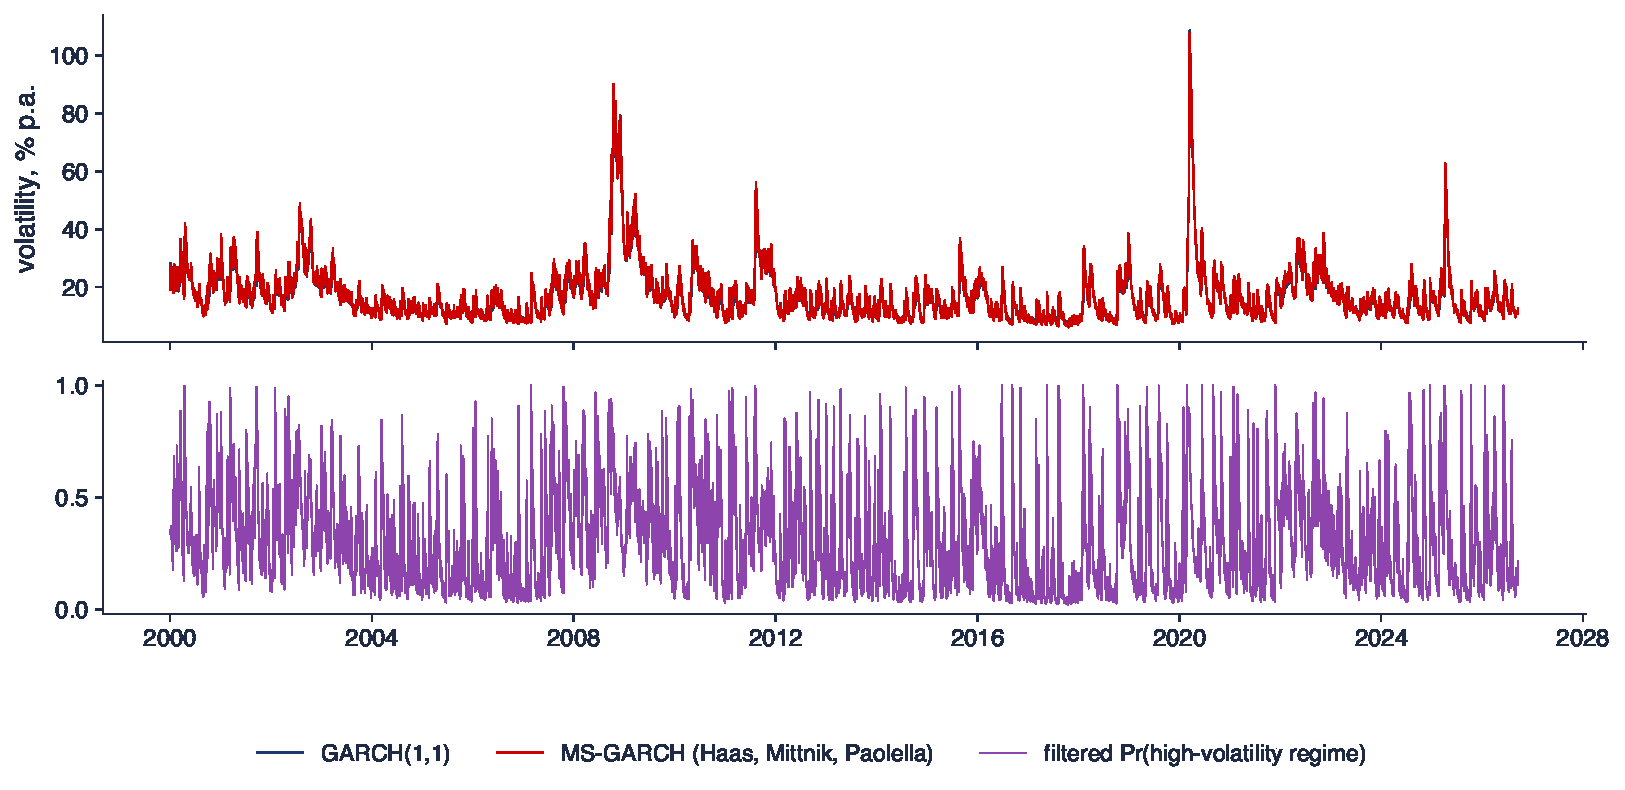
\includegraphics[width=0.97\textwidth,height=0.65\textheight,keepaspectratio]{ats_ch7_msgarch.pdf}
\end{center}
\vspace{-0.25cm}
\begin{itemize}
    \item Sus: volatilitatea condiționată anualizată, GARCH(1,1) și MS-GARCH (HMP, varianța amestecului); jos: probabilitatea filtrată a regimului de volatilitate ridicată
\end{itemize}
\quantlet{ATS\_ch7\_msgarch}{\qlurl{ATS_ch7_msgarch}}
\end{frame}

\begin{frame}{Interpretarea modelului MS-GARCH}
\itemsize{\small}
\begin{itemize}
    \item BIC preferă HMP (18317{,}5) față de GARCH (18475{,}0); regimul de volatilitate ridicată este activ în 21\% din zile
    \item Persistența cu un singur regim 0{,}981; în interiorul regimurilor 0{,}964 (calm) și 0{,}998 (volatilitate ridicată): regimurile nu elimină automat persistența, ci o mută acolo unde îi este locul
    \item Comprimarea lui Gray se potrivește mai slab aici (\ensuremath{-}9207{,}4): aproximarea nu este inofensivă
    \item Maximele locale sînt frecvente: puncte de pornire diferite dau împărțiri diferite în regimuri (raportați întotdeauna schema punctelor de pornire)
\end{itemize}
\end{frame}

\begin{frame}{Recapitulare: regimurile de volatilitate}
\itemsize{\small}
\begin{itemize}
    \item Regimurile de varianță și persistența GARCH sînt legate: raportați persistența din fiecare regim și pe cea a lanțului
    \item Dependența de traiectorie: comprimare (Gray, Klaassen) sau procese GARCH paralele (HMP)
    \item \atschlink{https://danpele.github.io/Advanced-Time-Series/RO/Cursuri/capitol8_volatilitate_avansata.pdf}{Capitolul 8} compară aceste modele cu măsurile realizate
\end{itemize}
\end{frame}


%=============================================================================
\section{Piețe bull și bear}
%=============================================================================

\begin{frame}{Regimuri pe piața de acțiuni: S\&P 500 și BET}
\itemsize{\footnotesize}
\begin{columns}[T]
\begin{column}{0.36\textwidth}
\centering

\includegraphics[height=0.34\textheight]{ch7_bvb_2024.jpg}\\[1mm]
\imgcap{Bursa de Valori București, 2024}
\imgcredit{https://commons.wikimedia.org/wiki/File:Bursa_de_Valori_București.jpg}{Foto: Corina Chitu (2024); CC BY-SA 4.0; Wikimedia Commons}
\end{column}
\begin{column}{0.62\textwidth}
\begin{itemize}
    \item Randamente logaritmice săptămînale, 2000--2026, MSIH(2): $r_t = \mu_{S_t} + \sigma_{S_t}\varepsilon_t$ \refMM, \refAT
    \item S\&P 500 (anualizat): calm, media 16{,}6\%, volatilitatea 10{,}9\%; agitat \ensuremath{-}20{,}6\%, 28{,}3\%
    \item BET: calm 20{,}1\%, 13{,}6\%; agitat 3{,}2\%, 39{,}9\%
    \item Durate (săptămîni), calm și agitat: S\&P 500 37 și 14; BET 33 și 12
\end{itemize}
\end{column}
\end{columns}
\end{frame}

\begin{frame}{Regimuri agitate pe două piețe}
\itemsize{\footnotesize}
\begin{center}
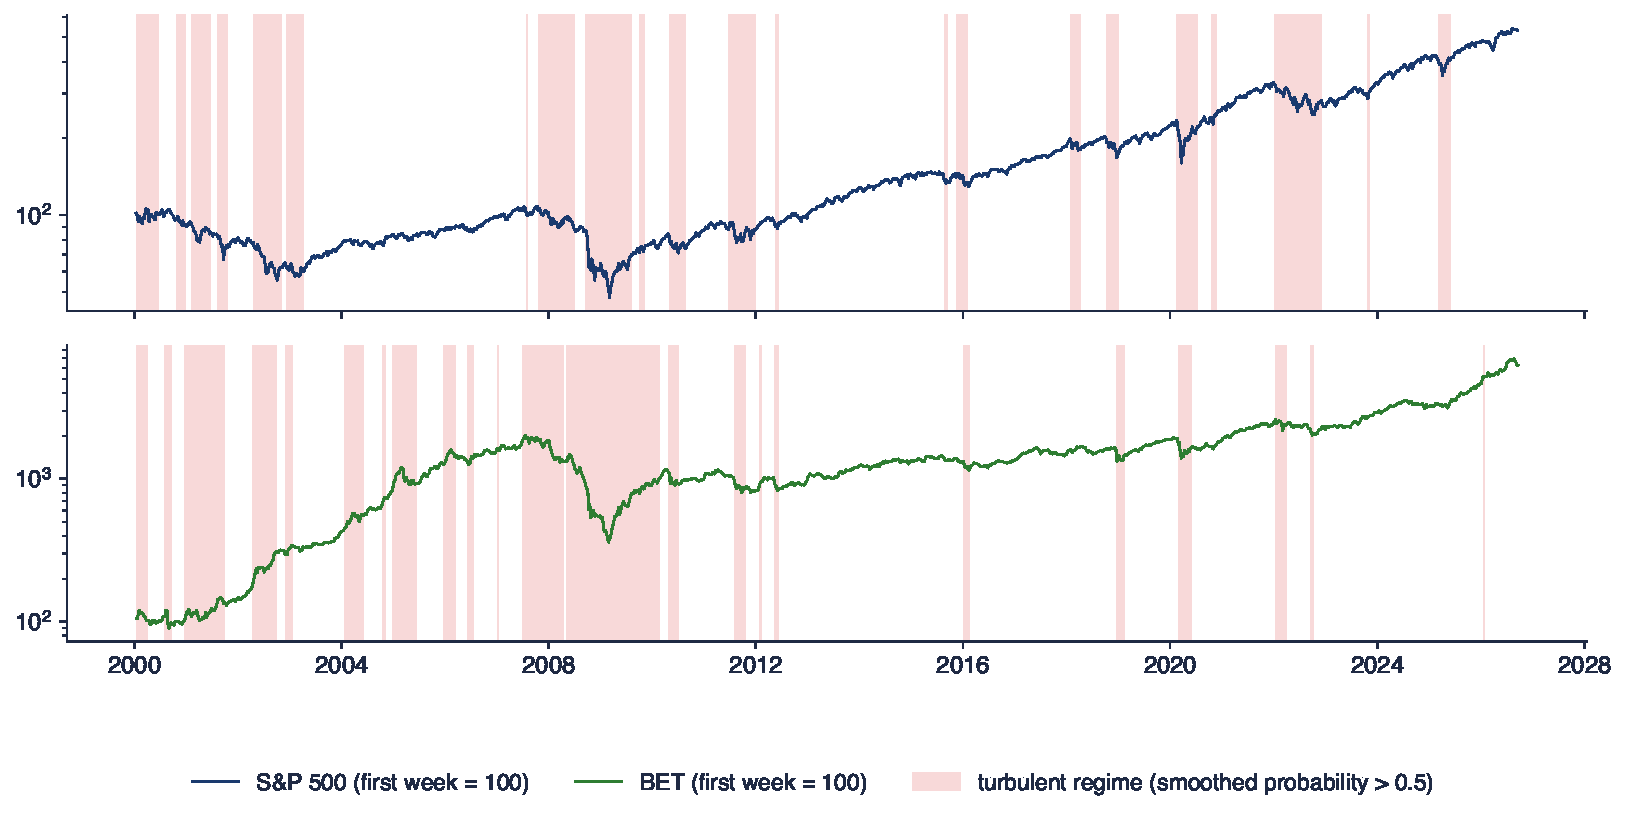
\includegraphics[width=0.97\textwidth,height=0.65\textheight,keepaspectratio]{ats_ch7_bullbear.pdf}
\end{center}
\vspace{-0.25cm}
\begin{itemize}
    \item Nivelurile indicilor pe scară logaritmică (prima săptămînă = 100); hașurat: probabilitatea netezită a regimului agitat peste 0,5; EM din 15 puncte de pornire și rafinare numerică (\texttt{statsmodels}: același $\ln L$)
\end{itemize}
\quantlet{ATS\_ch7\_bullbear}{\qlurl{ATS_ch7_bullbear}}
\end{frame}

\begin{frame}{Interpretarea regimurilor pieței de acțiuni}
\itemsize{\small}
\begin{itemize}
    \item Ponderea regimului agitat: S\&P 500 26\%, BET 25\%; corelația celor două probabilități 0{,}48; ambele agitate în 15\% din săptămîni
    \item Regimurile sînt mai ales regimuri de volatilitate: media regimului agitat este mai mică, dar estimată cu eroare mare
    \item $\ln L$: S\&P 500 \ensuremath{-}3019{,}3 (numpy) și \ensuremath{-}3019{,}3 (\texttt{statsmodels}); BET \ensuremath{-}3339{,}9 și \ensuremath{-}3339{,}9
    \item BET are episoade agitate proprii (politică internă, prăbușirea din 2007--2009), nu doar importate
\end{itemize}
\end{frame}

\begin{frame}{Regimuri și alocarea activelor, pe scurt}
\itemsize{\small}
\begin{itemize}
    \item \refAB
    \begin{itemize}
        \item cu schimbare de regim, portofoliile optime depind de probabilitățile curente ale regimurilor
        \item preferința pentru piața internă și valoarea diversificării internaționale se schimbă de la un regim la altul
    \end{itemize}
    \item Ponderea acțiunilor față de numerar în portofoliul medie--varianță, cu aversiunea la risc $\gamma = 5$: $w = \mu/(\gamma\sigma^2)$; $\mu$, $\sigma^2$: media și varianța săptămînale ale randamentului în regim
    \begin{itemize}
        \item S\&P 500: 2{,}79 în regimul calm, \ensuremath{-}0{,}51 în cel agitat, 0{,}39 cu momente constante
        \item cu momentele amestecului la un pas, ponderea se mișcă între \ensuremath{-}0{,}47 și 2{,}02
    \end{itemize}
    \item Rezerve: eroarea de estimare a mediilor pe regimuri este mare; cîștigurile în afara eșantionului trebuie testate (\atschlink{https://danpele.github.io/Advanced-Time-Series/RO/Cursuri/capitol1_evaluarea_prognozelor.pdf}{Capitolul 1}), iar costurile de tranzacționare incluse
    \item Aplicațiile de risc de piață (VaR și ES cu regimuri) sînt în \atschlink{https://danpele.github.io/MFM/RO/Cursuri/capitol7_var_expected_shortfall.pdf}{MFM, Capitolul 7}
\end{itemize}
\end{frame}


%=============================================================================
\section{Estimarea bayesiană}
%=============================================================================

\begin{frame}{Eșantionarea Gibbs cu augmentarea datelor}
\itemsize{\small}
\begin{itemize}
    \item Tratăm $S = (S_1, \dots, S_T)$ ca parametri \refAC: dat fiind $S$, modelul este un set de regresii; dat fiind $\theta$, $S$ este un lanț Markov ascuns
    \begin{itemize}
        \item 1. $S \mid \theta, Y$; 2. $\mathbf{P} \mid S$: rîndurile $\sim$ Dirichlet$(a_{i\cdot} + n_{i\cdot})$, $n_{ij}$ numărul de tranziții, $a_{ij}$ parametrii Dirichlet a priori
        \item 3. $\mu_j \mid \sigma_j^2, S, Y \sim$ Normală și $\sigma_j^2 \mid \mu_j, S, Y \sim$ inverse gamma: actualizări conjugate pe observațiile regimului $j$ (\atschlink{https://danpele.github.io/Advanced-Time-Series/RO/Cursuri/capitol5_bvar_modele_factoriale_nowcasting.pdf}{Capitolul 5})
    \end{itemize}
    \item \textbf{FFBS} \refChibB: extragem toată traiectoria odată: $S_T \sim \hat\xi_{T|T}$, apoi înapoi $\Pr(S_t = i \mid S_{t+1} = j, Y_t) \propto \hat\xi_{i,t|t}p_{ij}$
    \begin{itemize}
        \item eșantionarea cîte un $S_t$, dat fiind $S_{t-1}$ și $S_{t+1}$, are o amestecare (mixing) foarte lentă cînd regimurile sînt persistente
        \item analogul discret al simulation smoother-ului din \atschlink{https://danpele.github.io/Advanced-Time-Series/RO/Cursuri/capitol6_modele_spatiul_starilor_filtrare_bayesiana.pdf}{Capitolul 6} \refCK
    \end{itemize}
    \item Distribuțiile a priori țin $\sigma_j$ departe de 0 și $p_{ii}$ departe de frontieră: maximele degenerate ale verosimilității dispar
\end{itemize}
\end{frame}

\begin{frame}{Schimbarea etichetelor în MCMC și alegerea lui $K$}
\itemsize{\small}
\begin{itemize}
    \item \textbf{Eșantionatorul cu permutări aleatoare} \refFSa: permutăm aleator etichetele după fiecare iterație; eșantionatorul vizitează astfel toate cele $K!$ moduri
    \begin{itemize}
        \item rezultatul nerestricționat arată ce parametri separă regimurile; identificăm apoi prin restricția care le separă
        \item o restricție nepotrivită (de exemplu pe parametri aproape egali) taie un mod în două și deplasează ambele regimuri \refCHR
    \end{itemize}
    \item Alegerea lui $K$: verosimilitatea marginală $p(Y \mid K)$ din rezultatele Gibbs \refChibA, $\ln p(Y) = \ln f(Y \mid \theta^*) + \ln p(\theta^*) - \ln p(\theta^* \mid Y)$
    \begin{itemize}
        \item ordonata verosimilității vine din filtrul Hamilton; ordonata a posteriori din rulări Gibbs reduse
    \end{itemize}
    \item Modelele cu puncte de schimbare (Chib 1998) folosesc același eșantionator cu o matrice $\mathbf{P}$ superior triunghiulară
\end{itemize}
\end{frame}

\begin{frame}{Creșterea PIB-ului României: două regimuri prin eșantionare Gibbs}
\itemsize{\footnotesize}
\begin{center}
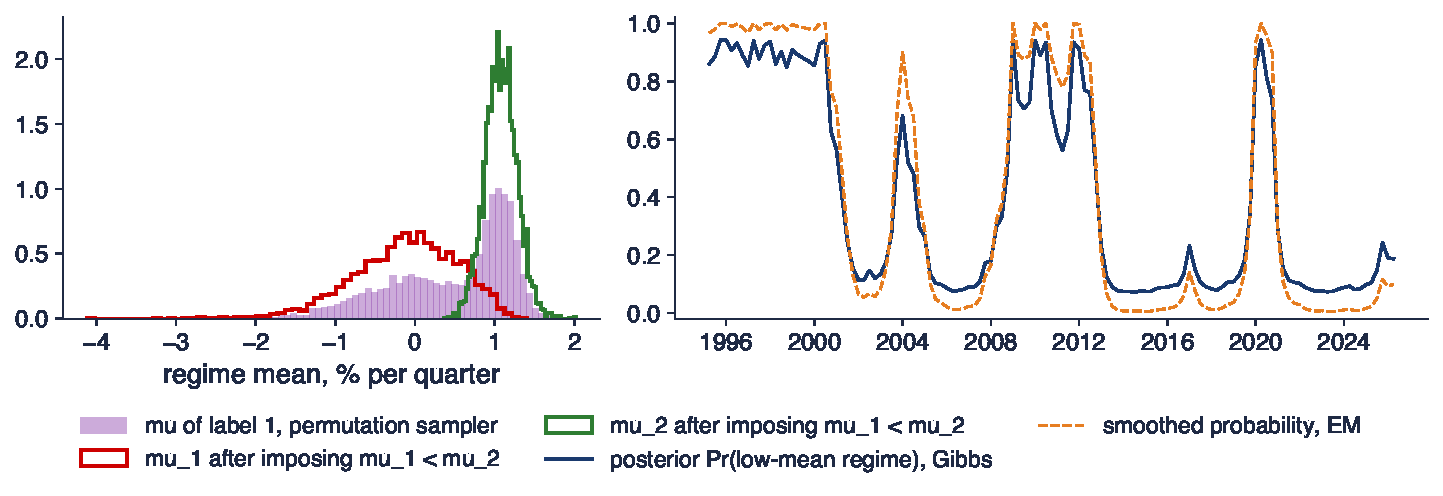
\includegraphics[width=0.97\textwidth,height=0.64\textheight,keepaspectratio]{ats_ch7_gibbs.pdf}
\end{center}
\vspace{-0.25cm}
\begin{itemize}
    \item Creșterea trimestrială, T2 1995--T2 2026 ($T = 125$), MSIH(2) fără termen AR; 5\,000 de extrageri după burn-in; stînga: eșantionatorul cu permutări, dreapta: eșantionatorul identificat prin $\mu_1 < \mu_2$
\end{itemize}
\quantlet{ATS\_ch7\_bayes}{\qlurl{ATS_ch7_bayes}}
\end{frame}

\begin{frame}{Interpretarea distribuției a posteriori}
\itemsize{\footnotesize}
\begin{itemize}
    \item Eșantionatorul cu permutări: eticheta 1 are media mai mare în 49\% din extrageri: histograma bimodală reprezintă cele două regimuri, nu două răspunsuri
    \item Identificat: $\mu_1$ \ensuremath{-}0{,}11 [\ensuremath{-}1{,}26; 0{,}87], $\sigma_1$ 3{,}80; $\mu_2$ 1{,}08 [0{,}76; 1{,}41], $\sigma_2$ 1{,}57 (intervale credibile de 90\%)
    \item $p_{11}$ 0{,}85 [0{,}73; 0{,}94], $p_{22}$ 0{,}91; EM: $\mu$ = 0{,}03 și 1{,}04, $p_{ii}$ = 0{,}90 și 0{,}94
    \item Mediile se suprapun, abaterile standard nu: regimurile sînt o eră volatilă (1995--2000, 2009--2012, 2020) și una stabilă; varianța este restricția de identificare mai bună
    \item Probabilitățile regimurilor a posteriori și cele din EM au corelația 0{,}99; distribuția a posteriori include și incertitudinea parametrilor, pe care traiectoria EM o ignoră
\end{itemize}
\end{frame}

\begin{frame}{Recapitulare: estimarea bayesiană}
\itemsize{\small}
\begin{itemize}
    \item Augmentarea datelor transformă modelul cu schimbare de regim în regresii conjugate plus FFBS
    \item Lăsați eșantionatorul să schimbe etichetele, apoi identificați cu parametrul care separă regimurile
    \item Verosimilitățile marginale compară valorile lui $K$ și modelele cu puncte de schimbare pe aceeași bază
\end{itemize}
\end{frame}


%=============================================================================
\section{Regimuri, memorie lungă și rupturi}
%=============================================================================

\begin{frame}{Comutările rare arată ca memoria lungă}
\itemsize{\small}
\begin{itemize}
    \item \refDI: $y_t = \mu_{S_t} + \varepsilon_t$ cu $p_{ii} = 1 - c/T^\delta$
    \begin{itemize}
        \item $c, \delta > 0$: comutările devin mai rare cînd $T$ crește
        \item varianța sumelor parțiale crește ca la un proces I($d$), $d > 0$
        \item autocorelațiile $\propto\lambda^k$, cu $\lambda \to 1$, scad atît de lent încît, în orice eșantion finit, par hiperbolice
    \end{itemize}
    \item Consecințe
    \begin{itemize}
        \item o estimație GPH sau Whittle locală semnificativă (\atschlink{https://danpele.github.io/Advanced-Time-Series/RO/Cursuri/capitol10_memorie_lunga_rough_volatility.pdf}{Capitolul 10}) nu deosebește integrarea fracționară de rupturile ocazionale sau de regimuri
        \item același lucru este valabil pentru persistența GARCH (secțiunea anterioară) și pentru testele de rădăcină unitară cu rupturi (\atschlink{https://danpele.github.io/Advanced-Time-Series/RO/Cursuri/capitol2_rupturi_structurale_modele_neliniare.pdf}{Capitolul 2})
    \end{itemize}
    \item Care descriere este „adevărată” contează mai puțin decît care prognozează mai bine în afara eșantionului
\end{itemize}
\end{frame}

\begin{frame}{Simulare: estimații GPH ale lui $d$ cu schimbare de regim}
\itemsize{\footnotesize}
\begin{center}
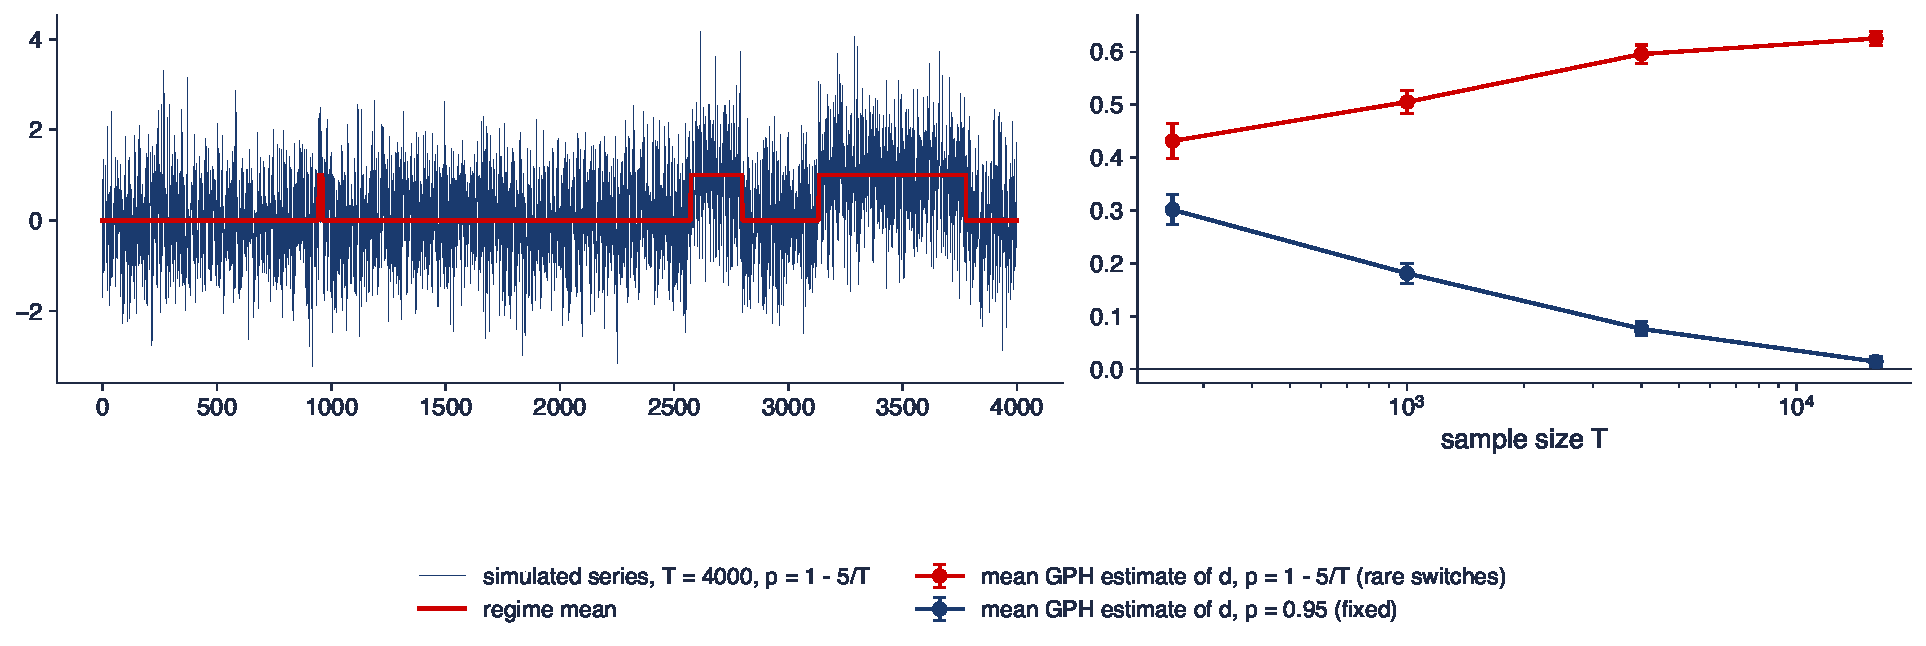
\includegraphics[width=0.97\textwidth,height=0.62\textheight,keepaspectratio]{ats_ch7_longmem.pdf}
\end{center}
\vspace{-0.25cm}
\begin{itemize}
    \item $y_t = \mu_{S_t} + \varepsilon_t$, $\mu \in \{0, 1\}$, $\sigma = 1$; media estimațiilor GPH ($m = T^{0{,}5}$) pe 200 de replicări, $\pm 2$ erori standard
\end{itemize}
\quantlet{ATS\_ch7\_longmem}{\qlurl{ATS_ch7_longmem}}
\end{frame}

\begin{frame}{Interpretarea simulării}
\itemsize{\small}
\begin{itemize}
    \item Comutări rare ($p = 1 - 5/T$): media $\hat d$ = 0{,}43; 0{,}51; 0{,}60; 0{,}63 pentru $T$ = 250; 1\,000; 4\,000; 16\,000: nu dispare cînd $T$ crește
    \item $p = 0{,}95$ fix: 0{,}30; 0{,}18; 0{,}08; 0{,}01: memorie scurtă, $\hat d \to 0$ pe măsură ce frecvențele folosite se apropie de zero
    \item Traiectoria din stînga are 6 comutări în 4000 de observații; autocorelația ei este 0{,}12 la lagul 50 și 0{,}06 la lagul 200
\end{itemize}
\end{frame}

\begin{frame}{Regimuri sau rupturi?}
\itemsize{\small}
\begin{itemize}
    \item O ruptură (\atschlink{https://danpele.github.io/Advanced-Time-Series/RO/Cursuri/capitol2_rupturi_structurale_modele_neliniare.pdf}{Capitolul 2}) este un regim care nu revine niciodată: $\mathbf{P}$ superior bidiagonală, $S_1 = 1$ \refChibC
    \begin{itemize}
        \item filtrul Hamilton și EM se aplică neschimbate; masca tranzițiilor ține tranzițiile interzise la zero
    \end{itemize}
    \item Regimurile recurente pun în comun informația din episoade: al doilea episod de inflație ridicată folosește parametrii primului
    \begin{itemize}
        \item rupturile cer un nou set de parametri pentru fiecare episod și nu spun nimic despre viitor
    \end{itemize}
    \item Comparăm cele două prin BIC sau verosimilitatea marginală; \refGP: rata reală a dobînzii din SUA este descrisă mai bine prin trei regimuri recurente decît printr-un proces stabil
\end{itemize}
\end{frame}

\begin{frame}{Regimurile inflației din România din 1997}
\itemsize{\footnotesize}
\begin{center}
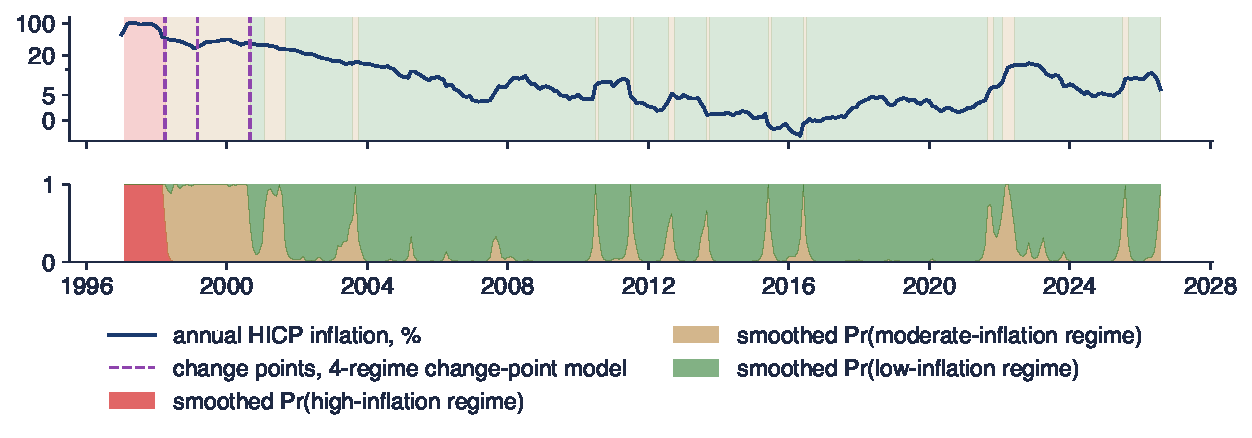
\includegraphics[width=0.97\textwidth,height=0.56\textheight,keepaspectratio]{ats_ch7_ro_infl.pdf}
\end{center}
\vspace{-0.25cm}
\begin{itemize}
    \item Inflația anuală IAPC, $100\ln(P_t/P_{t-12})$, din februarie 1997 ($T = 355$); MSIH(3)-AR(1), EM din 25 de puncte de pornire; linii întrerupte: punctele de schimbare ale modelului cu 4 regimuri; scară logaritmică simetrică
\end{itemize}
\quantlet{ATS\_ch7\_ro\_inflation}{\qlurl{ATS_ch7_ro_inflation}}
\end{frame}

\begin{frame}{Interpretarea regimurilor inflației}
\itemsize{\small}
\begin{itemize}
    \item Nivelurile regimurilor $\nu_j/(1 - \phi)$: 68{,}7\%, 17{,}8\% și 2{,}9\%; abaterea standard a șocurilor 10{,}58; 1{,}70 și 0{,}45 pp; $\phi = 0{,}971$: după 2001 cele două regimuri inferioare diferă mai ales prin volatilitate
    \item Regimul volatil revine la creșterea TVA din 2010, în 2022 și în 2025; probabilitățile filtrate în august 2026 (inflația 6{,}1\%): 0{,}00; 0{,}93; 0{,}07
    \item BIC preferă punctele de schimbare: 3 segmente 887{,}0, 4 segmente 897{,}5, schimbare de regim 934{,}1; punctele de schimbare ale modelului cu 4 segmente: aprilie 1998, martie 1999, septembrie 2000
    \item Interpretare: dezinflația a fost un proces într-un singur sens
    \begin{itemize}
        \item după 2000 un singur segment, foarte persistent, absoarbe creșterile din 2022 și 2025 ca șocuri
        \item dacă ele sînt un regim recurent se decide în afara eșantionului
    \end{itemize}
\end{itemize}
\end{frame}

\begin{frame}{Recapitulare: regimuri, memorie și rupturi}
\itemsize{\small}
\begin{itemize}
    \item Comutările rare imită memoria lungă: testele de memorie nu le pot deosebi
    \item Rupturile sînt regimuri nerecurente: același filtru, $\mathbf{P}$ restricționată
    \item Alegerea modelului este o întrebare de performanță în afara eșantionului
\end{itemize}
\end{frame}


%=============================================================================
\section{EUR/RON: regimuri ale cursului de schimb}
%=============================================================================

\begin{frame}{Regimurile cursului de schimb din România}
\itemsize{\footnotesize}
\begin{columns}[T]
\begin{column}{0.36\textwidth}
\centering
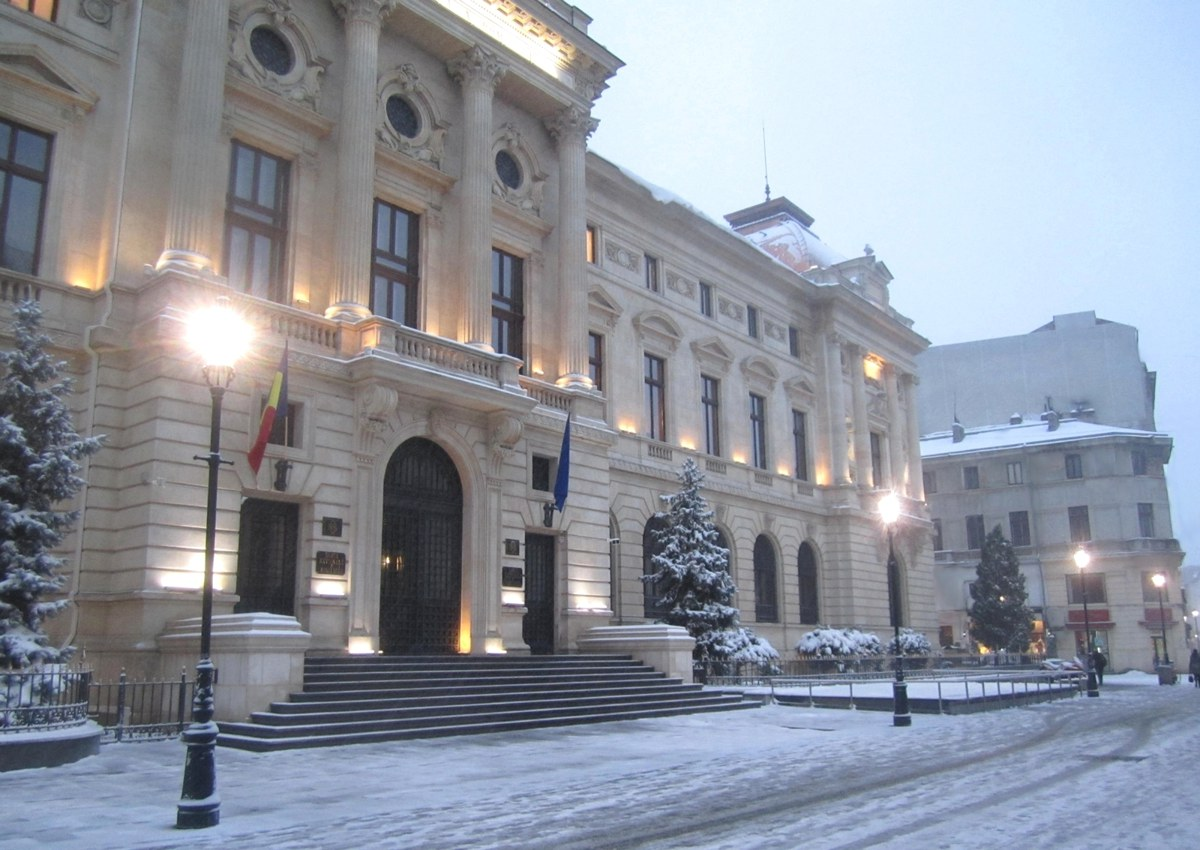
\includegraphics[height=0.34\textheight]{ch7_bnr_2014.jpg}\\[1mm]
\imgcap{Banca Națională a României, București, 2014}
\imgcredit{https://commons.wikimedia.org/wiki/File:Banca_Nationala_National_Bank_Bucharest_Bucuresti_Romania_2.JPG}{Foto: Crislia (2014); CC BY-SA 4.0; Wikimedia Commons}
\end{column}
\begin{column}{0.62\textwidth}
\begin{itemize}
    \item 1999--2005: depreciere graduală a leului vechi într-un regim de managed float
    \item Iulie 2005: denominarea (10\,000 ROL = 1 RON); august 2005: țintirea inflației, cu un regim de managed float; contul de capital complet liberalizat în 2006
    \item Episoade: octombrie 2008, 2011--2012, martie 2020, mai 2025 (alegerile prezidențiale și tensiunile fiscale)
    \item Modelul: variații logaritmice săptămînale, MSIH(3) ordonat după volatilitate; regimurile sînt rezultate ale politicii, nu regimul anunțat
\end{itemize}
\end{column}
\end{columns}
\end{frame}

\begin{frame}{Regimurile de volatilitate ale EUR/RON, 1999--2026}
\itemsize{\footnotesize}
\begin{center}
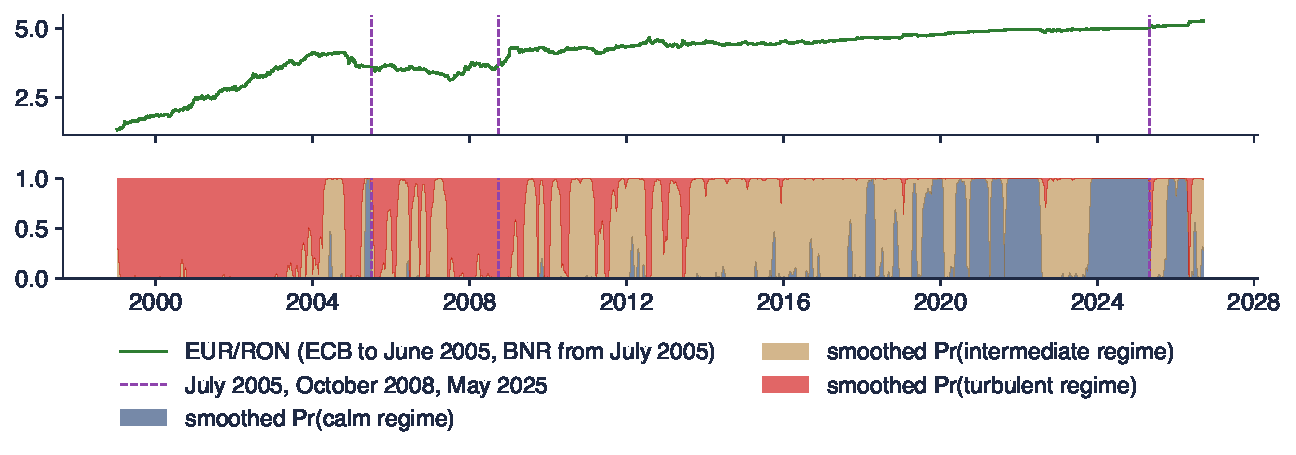
\includegraphics[width=0.97\textwidth,height=0.58\textheight,keepaspectratio]{ats_ch7_eurron.pdf}
\end{center}
\vspace{-0.25cm}
\begin{itemize}
    \item Sus: EUR/RON (cursul de referință BCE pînă în iunie 2005, BNR din iulie 2005); jos: probabilitățile netezite ale regimurilor calm, intermediar și agitat; $T = 1\,445$ de săptămîni
\end{itemize}
\quantlet{ATS\_ch7\_eurron}{\qlurl{ATS_ch7_eurron}}
\end{frame}

\begin{frame}{Interpretarea regimurilor EUR/RON}
\itemsize{\small}
\begin{itemize}
    \item Abaterea standard săptămînală pe regim: 0{,}07; 0{,}39 și 1{,}51\%; durate așteptate de 16; 17 și 20 de săptămîni
    \item Înainte de iulie 2005 regimul agitat cuprinde 87\% din săptămîni (deprecierea continuă a leului vechi, media 0{,}25\% pe săptămînă), după aceea 18\%; regimul calm trece de la 2\% la 25\%
    \item Probabilitatea regimului agitat atinge 1{,}00 în octombrie 2008--martie 2009 și 1{,}00 în primăvara lui 2025; cea mai mare variație săptămînală din 2025, 2{,}76\%, în săptămîna încheiată la 9 mai 2025
    \item EUR/RON a avut media 4{,}9773 în aprilie 2025 și era 5{,}2644 la sfîrșitul eșantionului: o schimbare de nivel urmată de revenirea la calm, cum prevede un regim de managed float
\end{itemize}
\end{frame}


%=============================================================================
\section{Prognoza cu modele cu schimbare de regim}
%=============================================================================

\begin{frame}{Prognozele unui model cu schimbare de regim}
\itemsize{\small}
\begin{itemize}
    \item Prognoza regimului: $\hat\xi_{T+h|T} = (\mathbf{P}')^h\hat\xi_{T|T}$, care converge spre $\boldsymbol\pi$ cu viteza $\lambda^h$
    \begin{itemize}
        \item la un pas: $f(y_{T+1} \mid Y_T) = \sum_j \hat\xi_{j,T+1|T}\,N(x_{T+1}'\beta_j, \sigma_j^2)$, un \textbf{amestec}: asimetric, cu cozi groase, posibil bimodal
    \end{itemize}
    \item La mai mulți pași, cu termeni AR: media nu este liniară în regimurile trecute (MSM) sau cere traiectoria regimurilor; simulăm traiectorii ale perechii $(S, y)$
    \item Evaluarea (\atschlink{https://danpele.github.io/Advanced-Time-Series/RO/Cursuri/capitol1_evaluarea_prognozelor.pdf}{Capitolul 1}): prognozele punctuale prin RMSE și Diebold--Mariano; densitățile prin scorul logaritmic, PIT și CRPS; probabilitățile regimurilor prin QPS
    \begin{itemize}
        \item QPS $= \frac2T\sum_t(\hat p_t - d_t)^2$ \refDR: scorul Brier al unei probabilități de recesiune $\hat p_t$ față de indicatorul NBER $d_t$ (1 în recesiune); 0 este perfect, 2 cel mai slab
    \end{itemize}
    \item \refCKr: modelele MS sînt rareori superioare modelelor AR liniare în prognozele punctuale ale PIB; valoarea lor stă în densități și în probabilitățile punctelor de întoarcere
\end{itemize}
\end{frame}

\begin{frame}{PIB-ul SUA: prognoze de densitate la un pas, 1990--2019}
\itemsize{\footnotesize}
\begin{center}
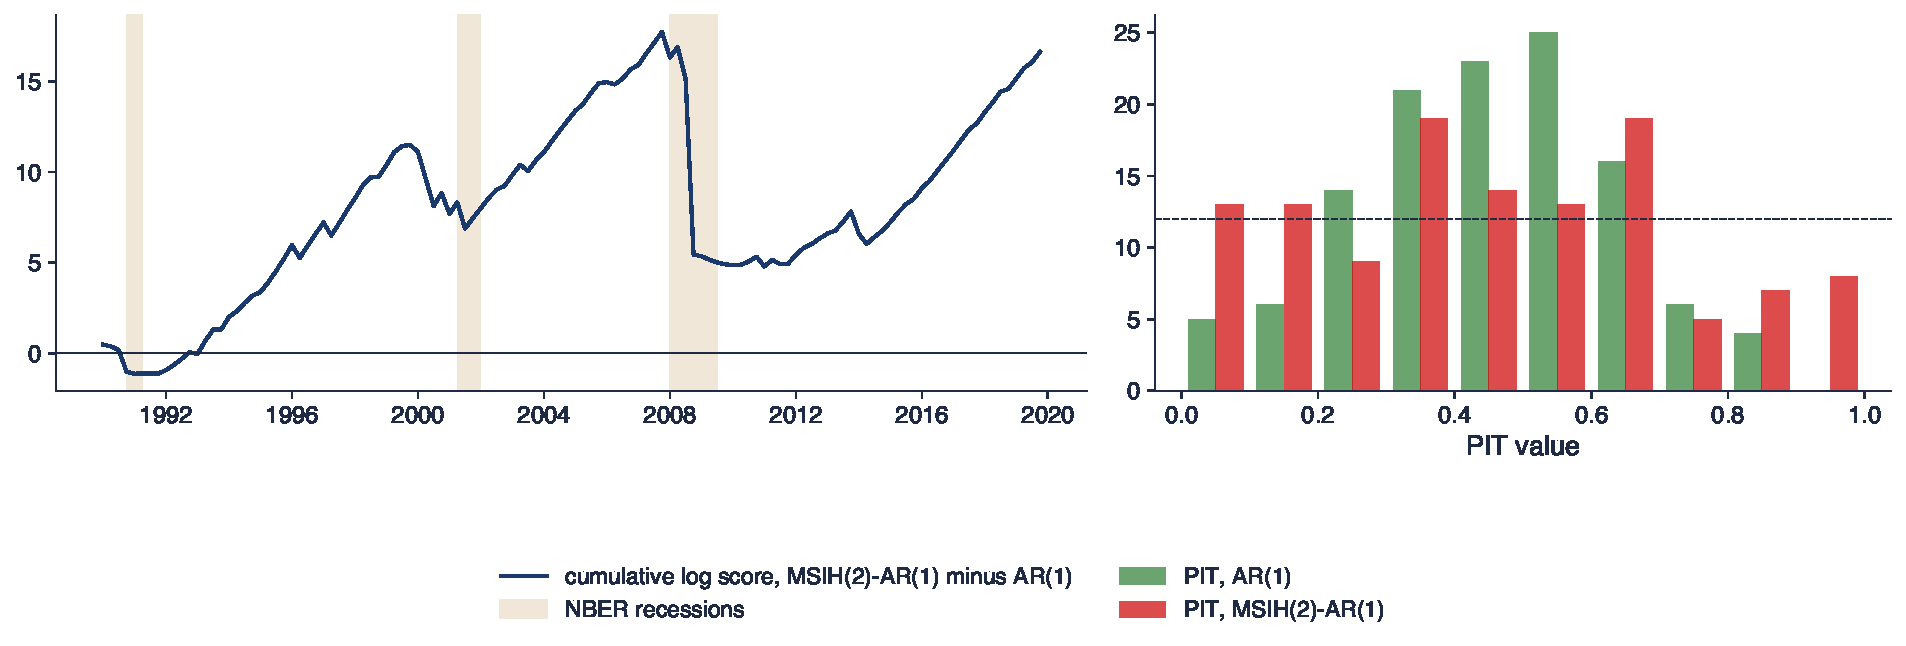
\includegraphics[width=0.97\textwidth,height=0.61\textheight,keepaspectratio]{ats_ch7_forecast.pdf}
\end{center}
\vspace{-0.25cm}
\begin{itemize}
    \item Fereastră extinsă din T2 1947, 120 de trimestre, AR(1) reestimat în fiecare trimestru, MSIH(2)-AR(1) la fiecare 4 trimestre (EM, pornind de la soluția anterioară); stînga: diferența cumulată a scorurilor logaritmice; dreapta: histogramele PIT (linia întreruptă: uniformă)
\end{itemize}
\quantlet{ATS\_ch7\_forecast}{\qlurl{ATS_ch7_forecast}}
\end{frame}

\begin{frame}{Interpretarea comparației prognozelor}
\itemsize{\small}
\begin{itemize}
    \item RMSE: AR(1) 0{,}554, MSIH(2)-AR(1) 0{,}558: prognozele punctuale sînt aproape identice, cum au găsit Clements și Krolzig
    \item Scorul logaritmic mediu: \ensuremath{-}1{,}028 față de \ensuremath{-}0{,}890; Diebold--Mariano pe diferență 1{,}16 ($p = 0{,}24$)
    \item Cîștigul vine din regimul de varianță: densitatea AR(1) este prea largă după 1984 (PIT concentrat la mijloc, KS $p < 0{,}001$); densitatea MS este mai aproape de uniformă, dar nici ea nu este calibrată (KS $p = 0{,}01$)
    \item Cîștigul cumulat de scor logaritmic înainte de 2008: 17{,}72; din 2008: \ensuremath{-}1{,}10: modelul cu regimuri cîștigă în perioadele calme și pierde în criză
\end{itemize}
\end{frame}

\begin{frame}{Recapitulare: prognoza}
\itemsize{\small}
\begin{itemize}
    \item Densitățile de prognoză sînt amestecuri; prognozele regimurilor converg spre probabilitățile ergodice
    \item Evaluați densitățile și probabilitățile regimurilor, nu doar RMSE
    \item Cîștigurile sînt episodice: testați-le în timp (teste de fluctuație, \atschlink{https://danpele.github.io/Advanced-Time-Series/RO/Cursuri/capitol1_evaluarea_prognozelor.pdf}{Capitolul 1})
\end{itemize}
\end{frame}


%=============================================================================
\section{AI în descoperirea științifică}
%=============================================================================

\begin{frame}{O întrebare deschisă}
\itemsize{\small}
\begin{itemize}
    \item Poate un model cu schimbare de regim să dateze în timp real recesiunile și regimurile inflației din România mai bine decît regulile simple și este episodul din 2025 un regim nou?
    \begin{itemize}
        \item formal: $H_0$: QPS egal pentru probabilitatea filtrată a regimului și pentru regula celor două trimestre negative, față de o cronologie de referință, pe trimestre preînregistrate
        \item infirmată de o diferență semnificativă pe trimestre pe care modelul nu le-a văzut, cu ediții ale PIB
    \end{itemize}
    \item Miza: România nu are un comitet oficial de datare a ciclului economic; politica reacționează la regimuri pe care le vede doar cu întîrziere
    \begin{itemize}
        \item literatura de pornire: \refHamA, \refCP, \refCKr, \refHamC
    \end{itemize}
\end{itemize}
\end{frame}

\begin{frame}{Bucla de cercetare cu un asistent AI}
\itemsize{\footnotesize}
\begin{itemize}
    \item Un asistent AI (un LLM precum Claude, ChatGPT, Gemini sau Copilot) accelerează fiecare etapă; Semantic Scholar și Elicit ajută la literatură
    \begin{itemize}
        \item \textbf{literatura}: \aiprompt{Listează articole recenzate care datează ciclurile economice ale țărilor din Europa Centrală și de Est cu modele Markov switching; dă DOI-urile.} Apoi verificați fiecare DOI pe Crossref
        \item \textbf{ipoteza}: \aiprompt{Ce specificație (MSM, MSIH, TVTP cu ce indicator avansat) ar trebui să separe recesiunile de erele de volatilitate în PIB-ul României?}
        \item \textbf{cod și replicare}: cereți un filtru Hamilton, apoi reproduceți întîi o cifră cunoscută (log-verosimilitatea lui Hamilton \ensuremath{-}181{,}26)
        \item \textbf{robustețe și critică}: \aiprompt{Joacă rolul unui recenzent ostil: enumeră felurile în care o datare a regimurilor poate fi un artefact al specificației sau al punctelor de pornire.}
    \end{itemize}
    \item Raportul: ce s-a cerut, ce s-a păstrat, ce s-a respins (AI\_USE.md, AI\_ERRORS.md)
\end{itemize}
\end{frame}

\begin{frame}{Verificări necesare}
\itemsize{\small}
\begin{itemize}
    \item Fiecare referință există și spune ce se afirmă (DOI-ul funcționează, titlul coincide, rezultatul se află în lucrare)
    \item Verosimilitatea este maximul global dintre multe puncte de pornire, iar regimul ales nu este degenerat
    \item Afirmațiile despre timpul real folosesc probabilități filtrate și ediții ale datelor, niciodată probabilități netezite
    \item Numărul de regimuri se testează prin bootstrap sau se alege printr-un criteriu fixat dinainte, nu prin numărarea gradelor de libertate ale unui $\chi^2$
    \item Semnificația fiecărui regim se verifică față de evenimente externe, nu se presupune din eticheta lui
\end{itemize}
\end{frame}

\begin{frame}{Mini studiu de caz: cît de robustă este o datare a recesiunilor?}
\itemsize{\footnotesize}
\begin{center}
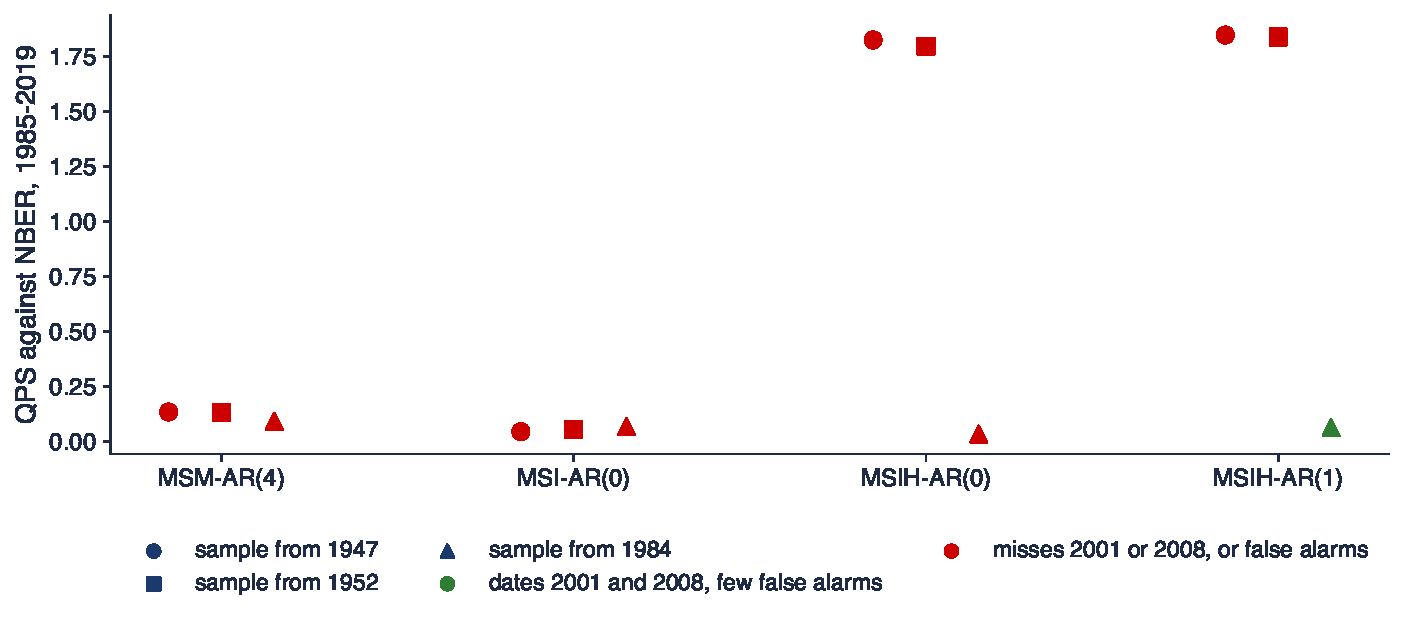
\includegraphics[width=0.97\textwidth,height=0.47\textheight,keepaspectratio]{ats_ch7_ai_case.pdf}
\end{center}
\vspace{-0.25cm}
\begin{itemize}
    \item Creșterea PIB-ului SUA: patru specificații $\times$ trei începuturi ale eșantionului, toate pînă în T4 2019; QPS al probabilității netezite a regimului cu media scăzută față de trimestrele NBER, 1985--2019
    \item QPS între 0{,}034 și 1{,}846 (o probabilitate constantă are scorul 0{,}145)
    \begin{itemize}
        \item 4 variante semnalează majoritatea trimestrelor: regimul lor cu media scăzută este Marea Moderație
        \item 1 din 12 datează atît 2001, cît și 2008 fără alarme false: un rezumat AI care raportează o singură variantă drept „datarea” greșește
    \end{itemize}
\end{itemize}
\quantlet{ATS\_ch7\_hamilton}{\qlurl{ATS_ch7_hamilton}}
\end{frame}

\begin{frame}{Idee de proiect}
\itemsize{\small}
\begin{itemize}
    \item \textbf{O cronologie a ciclului economic din România pe baza regimurilor}: întîi replicare, apoi extindere
    \begin{itemize}
        \item replicați: Tabelul I al lui Hamilton pe datele lui (log-verosimilitatea \ensuremath{-}181{,}26) și modelul TVTP al lui Filardo (\ensuremath{-}586{,}20)
        \item extindeți: PIB-ul și producția industrială ale României, MSM față de MSIH, TVTP cu ESI drept indicator avansat, alegerea bayesiană a lui $K$, probabilități filtrate în timp real
        \item preînregistrați: eșantionul, specificațiile, schema punctelor de pornire, cronologia de referință și comparația QPS
    \end{itemize}
    \item Livrabilele urmează regulile cursului: repository, raport, AI\_USE.md, AI\_ERRORS.md, susținere orală
\end{itemize}
\end{frame}


%=============================================================================
\section{Încheiere}
%=============================================================================

\begin{frame}{Idei de reținut}
\itemsize{\small}
\begin{itemize}
    \item Filtrul Hamilton și netezitorul Kim sînt recursii bayesiene exacte pentru o stare latentă discretă
    \item EM și verosimilitatea maximă numerică găsesc maxime locale și degenerate: multe puncte de pornire, apoi judecată
    \item Numărul de regimuri este o problemă de testare nestandard: bootstrap, Garcia, CHP sau criterii informaționale
    \item TVTP, MS-VAR și MS-GARCH dau regimurilor un conținut economic; eșantionarea Gibbs face vizibilă incertitudinea
    \item Regimurile, rupturile și memoria lungă sînt apropiate observațional; prognozele decid
\end{itemize}
\end{frame}

\begin{frame}{Autoevaluare}
\itemsize{\small}
\begin{columns}[T]
\begin{column}{0.56\textwidth}
\begin{block}{Întrebări}
\begin{itemize}
    \item De ce are nevoie netezitorul Kim de $\hat\xi_{t+1|t}$ la numitor?
    \item De ce are nevoie modelul MSM-AR(4) al lui Hamilton de 32 de stări?
    \item Ce trei condiții ale asimptoticii LR nu sînt îndeplinite la testarea unui regim față de două?
    \item De ce depinde de traiectorie verosimilitatea modelului MS-GARCH naiv?
    \item De ce poate o medie cu schimbare de regim să producă o estimație GPH pozitivă?
\end{itemize}
\end{block}
\end{column}
\begin{column}{0.40\textwidth}
\begin{block}{Urmează: \atschlink{https://danpele.github.io/Advanced-Time-Series/RO/Cursuri/capitol8_volatilitate_avansata.pdf}{Capitolul 8}}
\begin{itemize}
    \item Modelarea avansată a volatilității
    \item Măsuri realizate, HAR și GARCH multivariat
\end{itemize}
\end{block}
\end{column}
\end{columns}
\end{frame}


%=============================================================================
\section{Anexă}
%=============================================================================

\begin{frame}{Anexă: EM pentru lanțul Markov, pas cu pas}
\hypertarget{atsapp1}{}\atsappback{atssrc2}{Înapoi}
\itemsize{\small}
\begin{itemize}
    \item Log-verosimilitatea așteptată a datelor complete: $Q(\theta \mid \theta^{(m)}) = \sum_j\hat\xi_{j,1|T}\ln\rho_j + \sum_{t\ge2}\sum_{i,j}\hat\xi_{ij,t|T}\ln p_{ij} + \sum_t\sum_j\hat\xi_{j,t|T}\ln\eta_{jt}$
    \item Maximizăm $\sum_{t,j}\hat\xi_{ij,t|T}\ln p_{ij}$ cu $\sum_j p_{ij} = 1$: lagrangianul $\Rightarrow p_{ij} = \sum_t\hat\xi_{ij,t|T}/\sum_t\sum_k\hat\xi_{ik,t|T}$
    \item iar $\sum_k\hat\xi_{ik,t|T} = \hat\xi_{i,t-1|T}$; partea Gaussiană dă cele mai mici pătrate ponderate
    \item Monotonia: $\ln L(\theta) = Q(\theta \mid \theta^{(m)}) - H(\theta \mid \theta^{(m)})$, iar $H$ este maxim în $\theta^{(m)}$ (inegalitatea Gibbs) \refDLR
\end{itemize}
\end{frame}

\begin{frame}{Anexă: netezitorul Kim, pasul Markov}
\hypertarget{atsapp2}{}\atsappback{atssrc1}{Înapoi}
\itemsize{\small}
\begin{itemize}
    \item $\Pr(S_t = i \mid S_{t+1} = j, Y_T) = \dfrac{f(y_{t+1:T} \mid S_t = i, S_{t+1} = j, Y_t)\Pr(S_t = i \mid S_{t+1} = j, Y_t)}{f(y_{t+1:T} \mid S_{t+1} = j, Y_t)}$
    \item Dacă $y_{t+1:T}$ depinde de $S_t$ doar prin $S_{t+1}$ (adevărat pe starea extinsă), raportul densităților este 1
    \item Atunci $\Pr(S_t = i \mid S_{t+1} = j, Y_t) = \hat\xi_{i,t|t}p_{ij}/\hat\xi_{j,t+1|t}$; înmulțim cu $\hat\xi_{j,t+1|T}$ și sumăm după $j$
    \item Cu o stare continuă (spațiul stărilor cu schimbare de regim, \atschlink{https://danpele.github.io/Advanced-Time-Series/RO/Cursuri/capitol6_modele_spatiul_starilor_filtrare_bayesiana.pdf}{Capitolul 6}) raportul nu este 1: netezitorul Kim devine o aproximare
\end{itemize}
\end{frame}


%=============================================================================
\section{Bibliografie}
%=============================================================================

\begin{frame}{Bibliografie (1/4)}
\itemsize{\tiny}
\begin{itemize}
    \item Albert, J. H., \& Chib, S. (1993). Bayes inference via Gibbs sampling of autoregressive time series subject to Markov mean and variance shifts. \textit{Journal of Business \& Economic Statistics}, 11(1), 1--15. \href{https://doi.org/10.1080/07350015.1993.10509929}{doi:10.1080/07350015.1993.10509929}
    \item Ang, A., \& Bekaert, G. (2002). International asset allocation with regime shifts. \textit{The Review of Financial Studies}, 15(4), 1137--1187. \href{https://doi.org/10.1093/rfs/15.4.1137}{doi:10.1093/rfs/15.4.1137}
    \item Ang, A., \& Timmermann, A. (2012). Regime changes and financial markets. \textit{Annual Review of Financial Economics}, 4, 313--337. \href{https://doi.org/10.1146/annurev-financial-110311-101808}{doi:10.1146/annurev-financial-110311-101808}
    \item Baum, L. E., Petrie, T., Soules, G., \& Weiss, N. (1970). A maximization technique occurring in the statistical analysis of probabilistic functions of Markov chains. \textit{The Annals of Mathematical Statistics}, 41(1), 164--171. \href{https://doi.org/10.1214/aoms/1177697196}{doi:10.1214/aoms/1177697196}
    \item Bauwens, L., Preminger, A., \& Rombouts, J. V. K. (2010). Theory and inference for a Markov switching GARCH model. \textit{The Econometrics Journal}, 13(2), 218--244. \href{https://doi.org/10.1111/j.1368-423X.2009.00307.x}{doi:10.1111/j.1368-423X.2009.00307.x}
    \item Bollerslev, T. (1986). Generalized autoregressive conditional heteroskedasticity. \textit{Journal of Econometrics}, 31(3), 307--327. \href{https://doi.org/10.1016/0304-4076(86)90063-1}{doi:10.1016/0304-4076(86)90063-1}
    \item Carrasco, M., Hu, L., \& Ploberger, W. (2014). Optimal test for Markov switching parameters. \textit{Econometrica}, 82(2), 765--784. \href{https://doi.org/10.3982/ECTA8609}{doi:10.3982/ECTA8609}
    \item Carter, C. K., \& Kohn, R. (1994). On Gibbs sampling for state space models. \textit{Biometrika}, 81(3), 541--553. \href{https://doi.org/10.1093/biomet/81.3.541}{doi:10.1093/biomet/81.3.541}
    \item Celeux, G., Hurn, M., \& Robert, C. P. (2000). Computational and inferential difficulties with mixture posterior distributions. \textit{Journal of the American Statistical Association}, 95(451), 957--970. \href{https://doi.org/10.1080/01621459.2000.10474285}{doi:10.1080/01621459.2000.10474285}
    \item Chauvet, M., \& Piger, J. (2008). A comparison of the real-time performance of business cycle dating methods. \textit{Journal of Business \& Economic Statistics}, 26(1), 42--49. \href{https://doi.org/10.1198/073500107000000296}{doi:10.1198/073500107000000296}
    \item Chib, S. (1996). Calculating posterior distributions and modal estimates in Markov mixture models. \textit{Journal of Econometrics}, 75(1), 79--97. \href{https://doi.org/10.1016/0304-4076(95)01770-4}{doi:10.1016/0304-4076(95)01770-4}
    \item Chib, S. (1998). Estimation and comparison of multiple change-point models. \textit{Journal of Econometrics}, 86(2), 221--241. \href{https://doi.org/10.1016/S0304-4076(97)00115-2}{doi:10.1016/S0304-4076(97)00115-2}
\end{itemize}
\end{frame}

\begin{frame}{Bibliografie (2/4)}
\itemsize{\tiny}
\begin{itemize}
    \item Chib, S. (1995). Marginal likelihood from the Gibbs output. \textit{Journal of the American Statistical Association}, 90(432), 1313--1321. \href{https://doi.org/10.1080/01621459.1995.10476635}{doi:10.1080/01621459.1995.10476635}
    \item Cho, J. S., \& White, H. (2007). Testing for regime switching. \textit{Econometrica}, 75(6), 1671--1720. \href{https://doi.org/10.1111/j.1468-0262.2007.00809.x}{doi:10.1111/j.1468-0262.2007.00809.x}
    \item Clements, M. P., \& Krolzig, H.-M. (1998). A comparison of the forecast performance of Markov-switching and threshold autoregressive models of US GNP. \textit{The Econometrics Journal}, 1(1), C47--C75. \href{https://doi.org/10.1111/1368-423X.11004}{doi:10.1111/1368-423X.11004}
    \item Davies, R. B. (1987). Hypothesis testing when a nuisance parameter is present only under the alternative. \textit{Biometrika}, 74(1), 33--43. \href{https://doi.org/10.1093/biomet/74.1.33}{doi:10.1093/biomet/74.1.33}
    \item Dempster, A. P., Laird, N. M., \& Rubin, D. B. (1977). Maximum likelihood from incomplete data via the EM algorithm. \textit{Journal of the Royal Statistical Society: Series B}, 39(1), 1--22. \href{https://doi.org/10.1111/j.2517-6161.1977.tb01600.x}{doi:10.1111/j.2517-6161.1977.tb01600.x}
    \item Diebold, F. X., \& Inoue, A. (2001). Long memory and regime switching. \textit{Journal of Econometrics}, 105(1), 131--159. \href{https://doi.org/10.1016/S0304-4076(01)00073-2}{doi:10.1016/S0304-4076(01)00073-2}
    \item Diebold, F. X., Lee, J.-H., \& Weinbach, G. C. (1994). Regime switching with time-varying transition probabilities. In C. P. Hargreaves (Ed.), \textit{Nonstationary Time Series Analysis and Cointegration} (pp.\ 283--302). Oxford University Press. \href{https://doi.org/10.1093/oso/9780198773917.003.0010}{doi:10.1093/oso/9780198773917.003.0010}
    \item Diebold, F. X., \& Rudebusch, G. D. (1989). Scoring the leading indicators. \textit{The Journal of Business}, 62(3), 369--391. \href{https://doi.org/10.1086/296467}{doi:10.1086/296467}
    \item Ehrmann, M., Ellison, M., \& Valla, N. (2003). Regime-dependent impulse response functions in a Markov-switching vector autoregression model. \textit{Economics Letters}, 78(3), 295--299. \href{https://doi.org/10.1016/S0165-1765(02)00256-2}{doi:10.1016/S0165-1765(02)00256-2}
    \item Filardo, A. J. (1994). Business-cycle phases and their transitional dynamics. \textit{Journal of Business \& Economic Statistics}, 12(3), 299--308. \href{https://doi.org/10.1080/07350015.1994.10524545}{doi:10.1080/07350015.1994.10524545}
    \item Frühwirth-Schnatter, S. (2001). Markov chain Monte Carlo estimation of classical and dynamic switching and mixture models. \textit{Journal of the American Statistical Association}, 96(453), 194--209. \href{https://doi.org/10.1198/016214501750333063}{doi:10.1198/016214501750333063}
    \item Frühwirth-Schnatter, S. (2006). \textit{Finite Mixture and Markov Switching Models}. Springer. \href{https://doi.org/10.1007/978-0-387-35768-3}{doi:10.1007/978-0-387-35768-3}
\end{itemize}
\end{frame}

\begin{frame}{Bibliografie (3/4)}
\itemsize{\tiny}
\begin{itemize}
    \item Garcia, R. (1998). Asymptotic null distribution of the likelihood ratio test in Markov switching models. \textit{International Economic Review}, 39(3), 763--788. \href{https://doi.org/10.2307/2527399}{doi:10.2307/2527399}
    \item Garcia, R., \& Perron, P. (1996). An analysis of the real interest rate under regime shifts. \textit{The Review of Economics and Statistics}, 78(1), 111--125. \href{https://doi.org/10.2307/2109851}{doi:10.2307/2109851}
    \item Goldfeld, S. M., \& Quandt, R. E. (1973). A Markov model for switching regressions. \textit{Journal of Econometrics}, 1(1), 3--15. \href{https://doi.org/10.1016/0304-4076(73)90002-X}{doi:10.1016/0304-4076(73)90002-X}
    \item Gray, S. F. (1996). Modeling the conditional distribution of interest rates as a regime-switching process. \textit{Journal of Financial Economics}, 42(1), 27--62. \href{https://doi.org/10.1016/0304-405X(96)00875-6}{doi:10.1016/0304-405X(96)00875-6}
    \item Haas, M., Mittnik, S., \& Paolella, M. S. (2004). A new approach to Markov-switching GARCH models. \textit{Journal of Financial Econometrics}, 2(4), 493--530. \href{https://doi.org/10.1093/jjfinec/nbh020}{doi:10.1093/jjfinec/nbh020}
    \item Hamilton, J. D. (1990). Analysis of time series subject to changes in regime. \textit{Journal of Econometrics}, 45(1--2), 39--70. \href{https://doi.org/10.1016/0304-4076(90)90093-9}{doi:10.1016/0304-4076(90)90093-9}
    \item Hamilton, J. D. (1989). A new approach to the economic analysis of nonstationary time series and the business cycle. \textit{Econometrica}, 57(2), 357--384. \href{https://doi.org/10.2307/1912559}{doi:10.2307/1912559}
    \item Hamilton, J. D. (2016). Macroeconomic regimes and regime shifts. In J. B. Taylor \& H. Uhlig (Eds.), \textit{Handbook of Macroeconomics} (Vol.\ 2A, pp.\ 163--201). Elsevier. \href{https://doi.org/10.1016/bs.hesmac.2016.03.004}{doi:10.1016/bs.hesmac.2016.03.004}
    \item Hamilton, J. D., \& Susmel, R. (1994). Autoregressive conditional heteroskedasticity and changes in regime. \textit{Journal of Econometrics}, 64(1--2), 307--333. \href{https://doi.org/10.1016/0304-4076(94)90067-1}{doi:10.1016/0304-4076(94)90067-1}
    \item Hamilton, J. D. (1994). \textit{Time Series Analysis}. Princeton University Press. \href{https://doi.org/10.2307/j.ctv14jx6sm}{doi:10.2307/j.ctv14jx6sm}
    \item Hansen, B. E. (1992). The likelihood ratio test under nonstandard conditions: Testing the Markov switching model of GNP. \textit{Journal of Applied Econometrics}, 7(S1), S61--S82. \href{https://doi.org/10.1002/jae.3950070506}{doi:10.1002/jae.3950070506}
    \item Harding, D., \& Pagan, A. (2002). Dissecting the cycle: A methodological investigation. \textit{Journal of Monetary Economics}, 49(2), 365--381. \href{https://doi.org/10.1016/S0304-3932(01)00108-8}{doi:10.1016/S0304-3932(01)00108-8}
\end{itemize}
\end{frame}

\begin{frame}{Bibliografie (4/4)}
\itemsize{\tiny}
\begin{itemize}
    \item Hathaway, R. J. (1985). A constrained formulation of maximum-likelihood estimation for normal mixture distributions. \textit{The Annals of Statistics}, 13(2), 795--800. \href{https://doi.org/10.1214/aos/1176349557}{doi:10.1214/aos/1176349557}
    \item Kim, C.-J. (1994). Dynamic linear models with Markov-switching. \textit{Journal of Econometrics}, 60(1--2), 1--22. \href{https://doi.org/10.1016/0304-4076(94)90036-1}{doi:10.1016/0304-4076(94)90036-1}
    \item Kim, C.-J., \& Nelson, C. R. (1999). \textit{State-Space Models with Regime Switching: Classical and Gibbs-Sampling Approaches with Applications}. MIT Press. \href{https://doi.org/10.7551/mitpress/6444.001.0001}{doi:10.7551/mitpress/6444.001.0001}
    \item Klaassen, F. (2002). Improving GARCH volatility forecasts with regime-switching GARCH. \textit{Empirical Economics}, 27(2), 363--394. \href{https://doi.org/10.1007/s001810100100}{doi:10.1007/s001810100100}
    \item Krolzig, H.-M. (1997). \textit{Markov-Switching Vector Autoregressions: Modelling, Statistical Inference, and Application to Business Cycle Analysis}. Springer. \href{https://doi.org/10.1007/978-3-642-51684-9}{doi:10.1007/978-3-642-51684-9}
    \item Lamoureux, C. G., \& Lastrapes, W. D. (1990). Persistence in variance, structural change, and the GARCH model. \textit{Journal of Business \& Economic Statistics}, 8(2), 225--234. \href{https://doi.org/10.1080/07350015.1990.10509794}{doi:10.1080/07350015.1990.10509794}
    \item Maheu, J. M., \& McCurdy, T. H. (2000). Identifying bull and bear markets in stock returns. \textit{Journal of Business \& Economic Statistics}, 18(1), 100--112. \href{https://doi.org/10.1080/07350015.2000.10524851}{doi:10.1080/07350015.2000.10524851}
    \item Petropoulos, F., Apiletti, D., Assimakopoulos, V., Babai, M. Z., et al.\ (2022). Forecasting: Theory and practice. \textit{International Journal of Forecasting}, 38(3), 705--871. \href{https://doi.org/10.1016/j.ijforecast.2021.11.001}{doi:10.1016/j.ijforecast.2021.11.001}
    \item Rabiner, L. R. (1989). A tutorial on hidden Markov models and selected applications in speech recognition. \textit{Proceedings of the IEEE}, 77(2), 257--286. \href{https://doi.org/10.1109/5.18626}{doi:10.1109/5.18626}
    \item Sims, C. A., \& Zha, T. (2006). Were there regime switches in U.S. monetary policy? \textit{American Economic Review}, 96(1), 54--81. \href{https://doi.org/10.1257/000282806776157678}{doi:10.1257/000282806776157678}
    \item Stephens, M. (2000). Dealing with label switching in mixture models. \textit{Journal of the Royal Statistical Society: Series B}, 62(4), 795--809. \href{https://doi.org/10.1111/1467-9868.00265}{doi:10.1111/1467-9868.00265}
\end{itemize}
\end{frame}

\end{document}
